% Options for packages loaded elsewhere
\PassOptionsToPackage{unicode}{hyperref}
\PassOptionsToPackage{hyphens}{url}
%
\documentclass[
]{book}
\usepackage{amsmath,amssymb}
\usepackage{lmodern}
\usepackage{iftex}
\ifPDFTeX
  \usepackage[T1]{fontenc}
  \usepackage[utf8]{inputenc}
  \usepackage{textcomp} % provide euro and other symbols
\else % if luatex or xetex
  \usepackage{unicode-math}
  \defaultfontfeatures{Scale=MatchLowercase}
  \defaultfontfeatures[\rmfamily]{Ligatures=TeX,Scale=1}
\fi
% Use upquote if available, for straight quotes in verbatim environments
\IfFileExists{upquote.sty}{\usepackage{upquote}}{}
\IfFileExists{microtype.sty}{% use microtype if available
  \usepackage[]{microtype}
  \UseMicrotypeSet[protrusion]{basicmath} % disable protrusion for tt fonts
}{}
\makeatletter
\@ifundefined{KOMAClassName}{% if non-KOMA class
  \IfFileExists{parskip.sty}{%
    \usepackage{parskip}
  }{% else
    \setlength{\parindent}{0pt}
    \setlength{\parskip}{6pt plus 2pt minus 1pt}}
}{% if KOMA class
  \KOMAoptions{parskip=half}}
\makeatother
\usepackage{xcolor}
\IfFileExists{xurl.sty}{\usepackage{xurl}}{} % add URL line breaks if available
\IfFileExists{bookmark.sty}{\usepackage{bookmark}}{\usepackage{hyperref}}
\hypersetup{
  pdftitle={ちょっとニッチなR入門},
  pdfauthor={Tomokazu NOMURA},
  hidelinks,
  pdfcreator={LaTeX via pandoc}}
\urlstyle{same} % disable monospaced font for URLs
\usepackage{color}
\usepackage{fancyvrb}
\newcommand{\VerbBar}{|}
\newcommand{\VERB}{\Verb[commandchars=\\\{\}]}
\DefineVerbatimEnvironment{Highlighting}{Verbatim}{commandchars=\\\{\}}
% Add ',fontsize=\small' for more characters per line
\usepackage{framed}
\definecolor{shadecolor}{RGB}{248,248,248}
\newenvironment{Shaded}{\begin{snugshade}}{\end{snugshade}}
\newcommand{\AlertTok}[1]{\textcolor[rgb]{0.94,0.16,0.16}{#1}}
\newcommand{\AnnotationTok}[1]{\textcolor[rgb]{0.56,0.35,0.01}{\textbf{\textit{#1}}}}
\newcommand{\AttributeTok}[1]{\textcolor[rgb]{0.77,0.63,0.00}{#1}}
\newcommand{\BaseNTok}[1]{\textcolor[rgb]{0.00,0.00,0.81}{#1}}
\newcommand{\BuiltInTok}[1]{#1}
\newcommand{\CharTok}[1]{\textcolor[rgb]{0.31,0.60,0.02}{#1}}
\newcommand{\CommentTok}[1]{\textcolor[rgb]{0.56,0.35,0.01}{\textit{#1}}}
\newcommand{\CommentVarTok}[1]{\textcolor[rgb]{0.56,0.35,0.01}{\textbf{\textit{#1}}}}
\newcommand{\ConstantTok}[1]{\textcolor[rgb]{0.00,0.00,0.00}{#1}}
\newcommand{\ControlFlowTok}[1]{\textcolor[rgb]{0.13,0.29,0.53}{\textbf{#1}}}
\newcommand{\DataTypeTok}[1]{\textcolor[rgb]{0.13,0.29,0.53}{#1}}
\newcommand{\DecValTok}[1]{\textcolor[rgb]{0.00,0.00,0.81}{#1}}
\newcommand{\DocumentationTok}[1]{\textcolor[rgb]{0.56,0.35,0.01}{\textbf{\textit{#1}}}}
\newcommand{\ErrorTok}[1]{\textcolor[rgb]{0.64,0.00,0.00}{\textbf{#1}}}
\newcommand{\ExtensionTok}[1]{#1}
\newcommand{\FloatTok}[1]{\textcolor[rgb]{0.00,0.00,0.81}{#1}}
\newcommand{\FunctionTok}[1]{\textcolor[rgb]{0.00,0.00,0.00}{#1}}
\newcommand{\ImportTok}[1]{#1}
\newcommand{\InformationTok}[1]{\textcolor[rgb]{0.56,0.35,0.01}{\textbf{\textit{#1}}}}
\newcommand{\KeywordTok}[1]{\textcolor[rgb]{0.13,0.29,0.53}{\textbf{#1}}}
\newcommand{\NormalTok}[1]{#1}
\newcommand{\OperatorTok}[1]{\textcolor[rgb]{0.81,0.36,0.00}{\textbf{#1}}}
\newcommand{\OtherTok}[1]{\textcolor[rgb]{0.56,0.35,0.01}{#1}}
\newcommand{\PreprocessorTok}[1]{\textcolor[rgb]{0.56,0.35,0.01}{\textit{#1}}}
\newcommand{\RegionMarkerTok}[1]{#1}
\newcommand{\SpecialCharTok}[1]{\textcolor[rgb]{0.00,0.00,0.00}{#1}}
\newcommand{\SpecialStringTok}[1]{\textcolor[rgb]{0.31,0.60,0.02}{#1}}
\newcommand{\StringTok}[1]{\textcolor[rgb]{0.31,0.60,0.02}{#1}}
\newcommand{\VariableTok}[1]{\textcolor[rgb]{0.00,0.00,0.00}{#1}}
\newcommand{\VerbatimStringTok}[1]{\textcolor[rgb]{0.31,0.60,0.02}{#1}}
\newcommand{\WarningTok}[1]{\textcolor[rgb]{0.56,0.35,0.01}{\textbf{\textit{#1}}}}
\usepackage{longtable,booktabs,array}
\usepackage{calc} % for calculating minipage widths
% Correct order of tables after \paragraph or \subparagraph
\usepackage{etoolbox}
\makeatletter
\patchcmd\longtable{\par}{\if@noskipsec\mbox{}\fi\par}{}{}
\makeatother
% Allow footnotes in longtable head/foot
\IfFileExists{footnotehyper.sty}{\usepackage{footnotehyper}}{\usepackage{footnote}}
\makesavenoteenv{longtable}
\usepackage{graphicx}
\makeatletter
\def\maxwidth{\ifdim\Gin@nat@width>\linewidth\linewidth\else\Gin@nat@width\fi}
\def\maxheight{\ifdim\Gin@nat@height>\textheight\textheight\else\Gin@nat@height\fi}
\makeatother
% Scale images if necessary, so that they will not overflow the page
% margins by default, and it is still possible to overwrite the defaults
% using explicit options in \includegraphics[width, height, ...]{}
\setkeys{Gin}{width=\maxwidth,height=\maxheight,keepaspectratio}
% Set default figure placement to htbp
\makeatletter
\def\fps@figure{htbp}
\makeatother
\setlength{\emergencystretch}{3em} % prevent overfull lines
\providecommand{\tightlist}{%
  \setlength{\itemsep}{0pt}\setlength{\parskip}{0pt}}
\setcounter{secnumdepth}{5}
\usepackage{booktabs}
\ifLuaTeX
  \usepackage{selnolig}  % disable illegal ligatures
\fi
\usepackage[]{natbib}
\bibliographystyle{plainnat}

\title{ちょっとニッチなR入門}
\author{Tomokazu NOMURA}
\date{2021/01/18}

\begin{document}
\maketitle

{
\setcounter{tocdepth}{1}
\tableofcontents
}
\hypertarget{ux306fux3058ux3081ux306b}{%
\chapter{はじめに}\label{ux306fux3058ux3081ux306b}}

レポートや卒業論文で,Rを使ってデータ分析を行うための方法を説明する。Rについての解説ページは多数あるが,ここではとくに社会科学系分野におけるデータ分析を想定して説明する。体系的な内容というよりは,ほかの資料で説明されていることの隙間を埋めることを意図しているので,いろいろな資料と合わせて読んでほしい。

とくにおすすめのページは以下。

\begin{itemize}
\tightlist
\item
  立命館大学の森先生による「\href{https://tomoecon.github.io/R_for_graduate_thesis/}{卒業論文のためのR入門}」
\item
  関西大学の宋先生と高知工科大学の矢内先生による「\href{https://www.jaysong.net/RBook/}{私たちのR:ベストプラクティスの探求}」
\item
  北海道大学の土居先生による「\href{https://shohei-doi.github.io/quant_polisci/index.html}{Rで計量政治学入門}」
\end{itemize}

今後,ビジネスにおいても,学術研究においても,統計データを用いた分析は最も重要なツールになっていくと考えられる。統計学の理論を理解しておくことも重要だが,実際にデータを収集して整理し分析することができなければ,せっかくの理論も役に立たない。理論と実践をバランス良く学ぶことが重要。

データ分析というと,まずはExcelというイメージだと思う。実際,「分析ツール」などの機能を用いれば,Excelでも一通りの統計分析ができる。しかし,Excelは基本的にデータを分析するためのソフトウェアではないので,大規模なデータを扱ったり,高度な分析を行ったりするには向いていない。専用のソフトウェアを使えば,Excelよりも簡単に分析を行うことができるため,無料でもいろいろな統計分析専用のソフトウェアが利用できる現在,無理して何でもExcelでやろうとするメリットはない(Excelにはまた別の使い途がある)。

Rは統計データを分析するためのソフトウェア。完全に無料で利用でき,全世界に多数のユーザーがいるため,使い方についてさまざまな情報がインターネットで入手できる。また,最新の分析手法を用いるためのパッケージが絶えず開発されリリースされている。そのため,おカネをかけずに自力で高機能な統計ソフトを習得したいのであれば,Rをおすすめする。最初は少しとっつきにくいと感じるかもしれないが,慣れてくれば非常に柔軟な使い方ができる(統計分析だけでなく,論文を書いたりスライドを作ったりもできる)。

\hypertarget{rux3068rstudioux306eux30a4ux30f3ux30b9ux30c8ux30fcux30eb}{%
\chapter{RとRStudioのインストール}\label{rux3068rstudioux306eux30a4ux30f3ux30b9ux30c8ux30fcux30eb}}

\hypertarget{rux304cux4f7fux3048ux308bux30d1ux30bdux30b3ux30f3}{%
\section{Rが使えるパソコン}\label{rux304cux4f7fux3048ux308bux30d1ux30bdux30b3ux30f3}}

Rはオープン・ソースで開発されており,Windows,Mac,Linuxのいずれでも利用可能。Rそのものは性能の低いマシンでも十分に動作する(ただし,分析するデータの規模や用いる分析手法によってはある程度高性能なパソコンが必要になるかもしれない)。また,RStudioはRを便利に使うために必須と言えるソフトウェア。

これからパソコンを用意するという人には,Mac \textgreater{} Linux \textgreater{} Windowsの順でおすすめする。(わたしが)Rを使っていてトラブルが少ないのはMac。Linuxでも安定しているが,そもそも一般の人にLinuxは馴染みがないので,R以外の用途を考えると選択肢からは外れそう。Windowsは最初に少し設定が必要なのと,フォルダやファイル名に注意して利用する必要がある。といっても,いま使っているPCがWindowsであれば,買い換えるほどのものでもない。

Windowsの場合には,WSLという仮想環境のLinuxにRをインストールして使うことも可能。わたしは,WSLにRとRStudio Serverをインストールして,ChromeなどのブラウザでRStudioを使っている(けっこう快適)。

\hypertarget{ux30a4ux30f3ux30b9ux30c8ux30fcux30ebux65b9ux6cd5}{%
\section{インストール方法}\label{ux30a4ux30f3ux30b9ux30c8ux30fcux30ebux65b9ux6cd5}}

インストールの方法については,\href{https://yukiyanai.github.io/jp/resources/}{高知工科大学の矢内先生のホームページ}に,これ以上丁寧に説明することはできないというくらいに丁寧な解説スライドが公開されている。Ubuntu,Mac,Windows版があるので,これらを参考にインストールしてほしい。ただし,うまくいかなくても矢内先生に直接質問のメールを送ったりはしないこと。

\hypertarget{macux306bux30a4ux30f3ux30b9ux30c8ux30fcux30ebux3059ux308bux5834ux5408ux306eux88dcux8db3}{%
\subsection{Macにインストールする場合の補足}\label{macux306bux30a4ux30f3ux30b9ux30c8ux30fcux30ebux3059ux308bux5834ux5408ux306eux88dcux8db3}}

\begin{itemize}
\tightlist
\item
  Homebrewを使っている人は,Homebrewを使ってインストールする方が簡単。
\item
  Homebrewをインストールすれば,Command Line Toolsは自動で入る。
\item
  XCodeをインストールするとかなりのディスク容量を消費するので,ディスク容量に余裕がない場合にはCommand Line Toolsだけをインストールすることも可能。ターミナルで次のコマンドを実行することでインストールできる。
\end{itemize}

\begin{verbatim}
xcode-select --install
\end{verbatim}

\hypertarget{linuxux306bux30a4ux30f3ux30b9ux30c8ux30fcux30ebux3059ux308bux5834ux5408ux306eux88dcux8db3}{%
\subsection{Linuxにインストールする場合の補足}\label{linuxux306bux30a4ux30f3ux30b9ux30c8ux30fcux30ebux3059ux308bux5834ux5408ux306eux88dcux8db3}}

\begin{itemize}
\tightlist
\item
  Linux(WSLを含む)の場合には,RStudio Serverをインストールして,ChromeなどのブラウザでRStudioを使うこともできる。この方法だと,RやRStudioをインストールしたマシン(サーバー)以外のマシンからもブラウザを使って(サーバーの)RStudioにアクセスできるので便利。
\end{itemize}

\hypertarget{windowsux306bux30a4ux30f3ux30b9ux30c8ux30fcux30ebux3059ux308bux5834ux5408ux306eux88dcux8db3}{%
\subsection{Windowsにインストールする場合の補足}\label{windowsux306bux30a4ux30f3ux30b9ux30c8ux30fcux30ebux3059ux308bux5834ux5408ux306eux88dcux8db3}}

\begin{itemize}
\tightlist
\item
  RtoolsはとりあえずなくてもOk(パッケージをソースコードからビルドする場合に必要だが,ほとんどのパッケージはビルド済みのバイナリが提供されている)。
\item
  全角文字(とくに全角スペース)が含まれるフォルダ名の問題は,Rに限らずさまざまなソフトで問題を引き起こすので,可能であればWindowsのユーザー名を半角英数字だけに変更しておくのがおすすめ。
\end{itemize}

\hypertarget{rstudioux306eux753bux9762}{%
\section{RStudioの画面}\label{rstudioux306eux753bux9762}}

RStudioを起動すると,細かい違いはあれ下のような画面が表示されるはず。

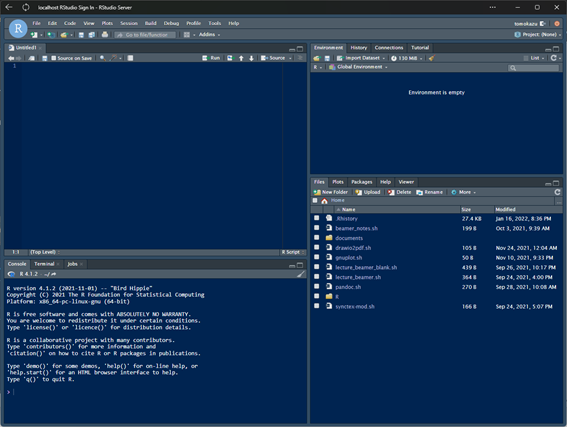
\includegraphics{RStudio.png}

デフォルトでは白背景の配色になっていると思うが,コードを書くときは黒背景の方が見やすいので変更している。見た目を変更するには,RStudioのメニューから{[}Tools{]}\textgreater{[}Global Options\ldots{]}を選び,Appearanceで設定する。長時間の作業を行う場合には,色やフォントによって作業効率や目の疲れ方がけっこう変わってくるので,いろいろ試して自分にあった設定にしよう。

RStudioの画面は,デフォルトで4ペイン(4分割)。最初はそのまま使っても良いと思うが,画面のレイアウトは比較的自由に変えることができるので,慣れてきたら自分が使いやすいように設定しよう。

各ペインにはタブが複数配置されている。まずは,よく使うものだけ説明する。

\begin{itemize}
\tightlist
\item
  Sourceペイン:デフォルトでは左上。何もファイルが開かれていない状態では最小化されているので,画面左上の+マークで新しいスクリプト・ファイル(R Script)を作成してみよう。
\item
  Consoleペイン:デフォルトでは左下。Rにコマンドを入力して実行する画面。
\item
  Environmentなどのペイン:デフォルトでは右上。Environmentタブには記憶されている変数やデータなどが表示される。Historyタブには実行したコマンドの履歴が表示され,選択して再度実行できる。
\item
  Filesなどのペイン:デフォルトでは右下。Filesタブには現在のディレクトリにあるファイルのリストが表示される。ファイル名をクリックすればファイルを開くことができる。RのソースコードなどやデータフレームはSourceペインで開かれる。Plotsタブはグラフが表示される場所。
\end{itemize}

Rで単発のコマンドを実行するときには,Consoleタブで行う。ただし,通常はスクリプト・ファイルにコマンドを書いて一つずつ実行していったり,いくつかのコマンドをまとめて実行したりすることが多い。Consoleでコマンドを実行した場合にも,Histroyタブからスクリプト・ファイルへと実行したコマンドを貼り付けておくと良い。そうすれば,いつでも作業を最初から再現できる。研究では,結果を再現できることが極めて重要。再現性を担保できることは,ExcelではなくRを使うメリットの一つ。

スクリプト・ファイルに書かれたコマンドを実行する場合,Ctrlを押しながらEnterを押す。範囲が選択されていない場合には,カーソルのある行(コマンドが複数行にまたがっていてもOk)が実行される。範囲を選択してCtrl+Enterを押せば,選択された範囲のコードが順に実行される。

\hypertarget{ux30d8ux30ebux30d7ux306eux53c2ux7167}{%
\section{ヘルプの参照}\label{ux30d8ux30ebux30d7ux306eux53c2ux7167}}

Rのコマンド・ヘルプは?のあとにコマンド名を入力すれば参照できる。ヘルプは,Helpタブ(デフォルトでは右下のペイン)に表示される。知らないコマンドが出てきたらまずはヘルプを読む。英語が苦手でもDeepLで翻訳すればだいたい読める。

たとえば,table関数のヘルプを読みたければ,

\begin{verbatim}
?table
\end{verbatim}

\hypertarget{ux30c1ux30e5ux30fcux30c8ux30eaux30a2ux30ebux306eux5b9fux884c}{%
\section{チュートリアルの実行}\label{ux30c1ux30e5ux30fcux30c8ux30eaux30a2ux30ebux306eux5b9fux884c}}

右上のペインにTutorialというタブがあり,そこからRのチュートリアル・レッスンを受けられる。チュートリアルを実行するためのパッケージをインストールするのに時間がかかるが,とりあえず一通り実行してみると,Rの使い方についてのイメージを持つことができるはず。

\hypertarget{ux30d1ux30c3ux30b1ux30fcux30b8ux306eux30a4ux30f3ux30b9ux30c8ux30fcux30eb}{%
\section{パッケージのインストール}\label{ux30d1ux30c3ux30b1ux30fcux30b8ux306eux30a4ux30f3ux30b9ux30c8ux30fcux30eb}}

Rは本体にパッケージを追加することで,機能を拡張することができる。パッケージをインストールするには,install.packages関数を用いる。とくに,tidyverseパッケージは必ず利用することになるので,インストールしておこう。

\begin{Shaded}
\begin{Highlighting}[]
\FunctionTok{install.packages}\NormalTok{(}\StringTok{"tidyverse"}\NormalTok{)}
\end{Highlighting}
\end{Shaded}

パッケージはインストールするだけでは使えないので,毎回読み込む必要がある。パッケージを読み込むにはlibrary関数を使う。

\begin{Shaded}
\begin{Highlighting}[]
\FunctionTok{library}\NormalTok{(tidyverse)}
\end{Highlighting}
\end{Shaded}

\hypertarget{rux306bux304aux3051ux308bux30aaux30d6ux30b8ux30a7ux30afux30c8}{%
\chapter{Rにおけるオブジェクト}\label{rux306bux304aux3051ux308bux30aaux30d6ux30b8ux30a7ux30afux30c8}}

\hypertarget{ux6570ux5024ux3068ux6587ux5b57ux5217}{%
\section{数値と文字列}\label{ux6570ux5024ux3068ux6587ux5b57ux5217}}

Rでは,さまざまな情報を記憶するための「箱」のことをオブジェクトという。オブジェクトには数値や文字,ベクトル,データフレームなどを記憶させることができる。

オブジェクトの名前は比較的自由につけることができる。日本語(漢字)を使うこともできるが,変数名に使うのはなるべく英数字とアンダースコア''\_``だけにした方が良い。

たとえば,a というオブジェクトに2という数値,bというオブジェクトに1.5という数値を記憶させてみよう。

\begin{Shaded}
\begin{Highlighting}[]
\NormalTok{a }\OtherTok{\textless{}{-}} \DecValTok{2}
\NormalTok{b }\OtherTok{\textless{}{-}} \FloatTok{2.5}
\end{Highlighting}
\end{Shaded}

このような操作を「代入」という。代入が正しく行われたかどうかを確認してみよう。

\begin{Shaded}
\begin{Highlighting}[]
\NormalTok{a}
\end{Highlighting}
\end{Shaded}

\begin{verbatim}
## [1] 2
\end{verbatim}

\begin{Shaded}
\begin{Highlighting}[]
\NormalTok{b}
\end{Highlighting}
\end{Shaded}

\begin{verbatim}
## [1] 2.5
\end{verbatim}

\begin{Shaded}
\begin{Highlighting}[]
\NormalTok{a}\SpecialCharTok{+}\NormalTok{b}
\end{Highlighting}
\end{Shaded}

\begin{verbatim}
## [1] 4.5
\end{verbatim}

\begin{Shaded}
\begin{Highlighting}[]
\NormalTok{a}\SpecialCharTok{*}\NormalTok{b}
\end{Highlighting}
\end{Shaded}

\begin{verbatim}
## [1] 5
\end{verbatim}

a, bにそれぞれ2,2.5という数値が代入されていて,a,bを用いた計算もできることがわかる。

また,RStudioの''Environment''タブにオブジェクト名a,bと代入された値が表示されていることもあわせて確認しよう。

\begin{figure}
\centering
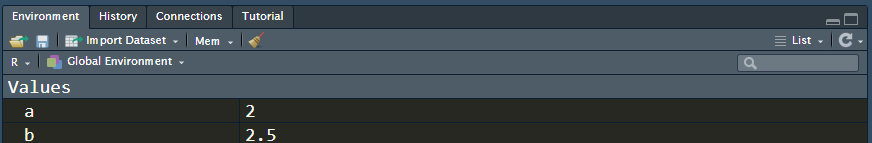
\includegraphics{ab.png}
\caption{Environment}
\end{figure}

オブジェクトには,数値だけではなく,文字列を代入することもできる。文字列は,ダブルクオーテーション''\,``で括る。

\begin{Shaded}
\begin{Highlighting}[]
\NormalTok{name }\OtherTok{\textless{}{-}} \StringTok{"大阪 太郎"}
\NormalTok{gender }\OtherTok{\textless{}{-}} \StringTok{"男"}
\NormalTok{age }\OtherTok{\textless{}{-}} \StringTok{"20"}
\end{Highlighting}
\end{Shaded}

\begin{figure}
\centering
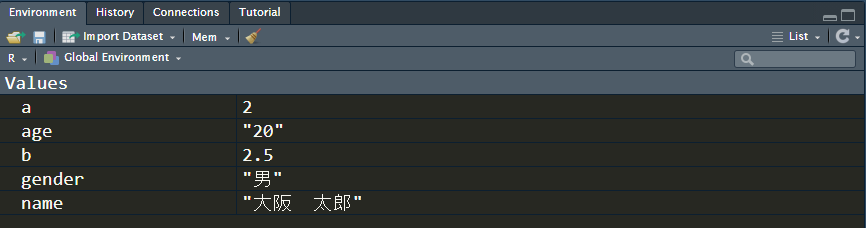
\includegraphics{moji.png}
\caption{Environment}
\end{figure}

nameというオブジェクトには''大阪 太郎''という文字列,genderというオブジェクトには''男''という文字列,ageというオブジェクトには''20''という文字列が代入れていることがわかる。

ここで,ageに代入されている''20''は,20という数値ではなく,文字列として扱われていることに注意しよう。そのため,ageを数値として計算に用いることはできず,下のようなエラーとなる。

\begin{Shaded}
\begin{Highlighting}[]
\NormalTok{age}\SpecialCharTok{+}\DecValTok{10}
\end{Highlighting}
\end{Shaded}

\begin{verbatim}
## Error in age + 10:  二項演算子の引数が数値ではありません
\end{verbatim}

オブジェクトは代入されるものによっていくつかの型(Type)に分類される。ここでは,a,bは数値型(numeric),name,gender,ageは文字列型(character)となる。

EnvironmentタブをList表示からGrid表示に切り替えれば,オブジェクトの型が表示される。

\begin{figure}
\centering
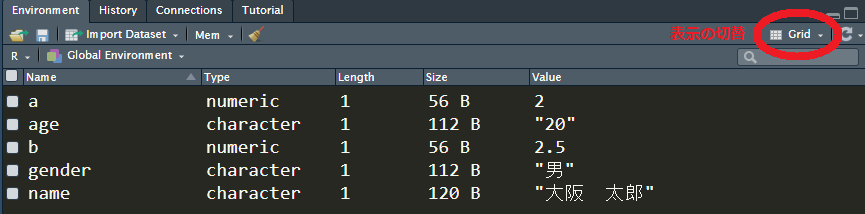
\includegraphics{grid.png}
\caption{Grid表示}
\end{figure}

文字列型のオブジェクトを数値型に変換したい場合には,as.numeric()関数を用いる。

\begin{Shaded}
\begin{Highlighting}[]
\FunctionTok{as.numeric}\NormalTok{(age)}\SpecialCharTok{+}\DecValTok{10}
\end{Highlighting}
\end{Shaded}

\begin{verbatim}
## [1] 30
\end{verbatim}

この例ではageは文字列型だが,as.numeric(age)でageを数値型に変換している。数値型に変換されているので,計算を行うことができる。

逆に数値型のオブジェクトを文字列型に変換するには,as.character()関数を用いる。

\hypertarget{ux30d9ux30afux30c8ux30eb}{%
\section{ベクトル}\label{ux30d9ux30afux30c8ux30eb}}

1つのオブジェクトに,複数の数値や文字列を代入することもできる。複数の数値や文字列が格納されたオブジェクトをベクトルという。たとえば,nameというベクトルに3人の名前を代入し,ageというベクトルに3人の年齢を代入してみよう。ベクトルは,c(要素1,要素2,\ldots)で表す。

\begin{Shaded}
\begin{Highlighting}[]
\NormalTok{name }\OtherTok{\textless{}{-}} \FunctionTok{c}\NormalTok{(}\StringTok{"大阪 太郎"}\NormalTok{,}\StringTok{"兵庫 次郎"}\NormalTok{,}\StringTok{"京都 花子"}\NormalTok{)}
\NormalTok{age }\OtherTok{\textless{}{-}} \FunctionTok{c}\NormalTok{(}\DecValTok{19}\NormalTok{,}\DecValTok{21}\NormalTok{,}\DecValTok{20}\NormalTok{)}
\end{Highlighting}
\end{Shaded}

nameとageの内容を確認してみよう。

\begin{Shaded}
\begin{Highlighting}[]
\NormalTok{name}
\end{Highlighting}
\end{Shaded}

\begin{verbatim}
## [1] "大阪 太郎" "兵庫 次郎" "京都 花子"
\end{verbatim}

\begin{Shaded}
\begin{Highlighting}[]
\NormalTok{age}
\end{Highlighting}
\end{Shaded}

\begin{verbatim}
## [1] 19 21 20
\end{verbatim}

nameとageの内容が先ほどのものと置き換わっていることがわかる。Rでは既存のオブジェクトに改めて別の内容を代入すると,中身が置き換えられる。

\begin{figure}
\centering
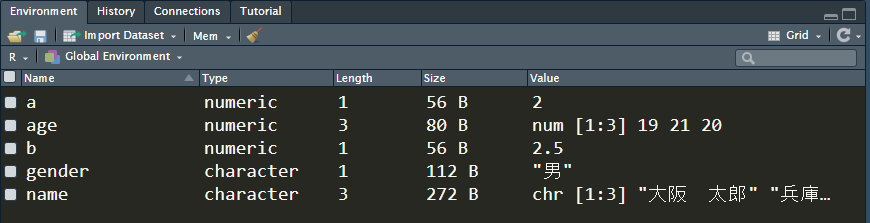
\includegraphics{vector.png}
\caption{ベクトル}
\end{figure}

Environmentタブで確認すると,nameとageのLengthが1から3へと変わっていることがわかる。Lengthはベクトルの長さ(要素の数)を表す。

ベクトルから1つの要素を取り出すには,ベクトル名のあとに{[}要素番号{]}をつける。ただし,ベクトルの要素番号は1から始まることに注意しよう(言語によっては0から始まるものもあるので混乱しないよう)。たとえば,nameというベクトルの2番目の要素を取り出すのであれば,下のように書く。

\begin{Shaded}
\begin{Highlighting}[]
\NormalTok{name[}\DecValTok{2}\NormalTok{]}
\end{Highlighting}
\end{Shaded}

\begin{verbatim}
## [1] "兵庫 次郎"
\end{verbatim}

\hypertarget{ux30d5ux30a1ux30afux30bfux30fc}{%
\section{ファクター}\label{ux30d5ux30a1ux30afux30bfux30fc}}

ベクトルの要素が,性別や都道府県などカテゴリを表すデータの場合には,factor型のベクトルを用いる。

たとえば,性別を格納するベクトルgenderを作成し,factor型に変換してみよう。ベクトルをfactor型に変換するにはas.factor()関数を用いる。

\begin{Shaded}
\begin{Highlighting}[]
\NormalTok{gender }\OtherTok{\textless{}{-}} \FunctionTok{c}\NormalTok{(}\StringTok{"男"}\NormalTok{,}\StringTok{"女"}\NormalTok{,}\StringTok{"男"}\NormalTok{)}
\NormalTok{gender }\OtherTok{\textless{}{-}} \FunctionTok{as.factor}\NormalTok{(gender)}
\end{Highlighting}
\end{Shaded}

genderの内容を確認してみよう。

\begin{Shaded}
\begin{Highlighting}[]
\NormalTok{gender}
\end{Highlighting}
\end{Shaded}

\begin{verbatim}
## [1] 男 女 男
## Levels: 女 男
\end{verbatim}

これは,ベクトルの内容は3人の性別(男,女,男)で,ベクトルの要素は「女」と「男」の2つのレベルに分類されていることを示している。

factor型のオブジェクトは,数値型へと変換することができる。factor型のオブジェクトgenderを数値型に変換して,新しいオブジェクトgender\_numに代入してみよう。

\begin{Shaded}
\begin{Highlighting}[]
\NormalTok{gender\_num }\OtherTok{\textless{}{-}} \FunctionTok{as.numeric}\NormalTok{(gender)}
\NormalTok{gender\_num}
\end{Highlighting}
\end{Shaded}

\begin{verbatim}
## [1] 2 1 2
\end{verbatim}

性別が番号(女:1,男:2)に変換されていることがわかる。このとき振られる番号は,Levelsで表示される順番となる。レベルの順番は,factor関数でlevelsを指定することで変更可能。

\begin{Shaded}
\begin{Highlighting}[]
\NormalTok{gender }\OtherTok{\textless{}{-}} \FunctionTok{factor}\NormalTok{(gender, }\AttributeTok{levels=}\FunctionTok{c}\NormalTok{(}\StringTok{"男"}\NormalTok{,}\StringTok{"女"}\NormalTok{))}
\NormalTok{gender}
\end{Highlighting}
\end{Shaded}

\begin{verbatim}
## [1] 男 女 男
## Levels: 男 女
\end{verbatim}

\begin{Shaded}
\begin{Highlighting}[]
\FunctionTok{as.numeric}\NormalTok{(gender)}
\end{Highlighting}
\end{Shaded}

\begin{verbatim}
## [1] 1 2 1
\end{verbatim}

\hypertarget{ux5206ux985eux306eux7d50ux5408}{%
\subsection{分類の結合}\label{ux5206ux985eux306eux7d50ux5408}}

いくつかのカテゴリを1つにまとめて,factor型ベクトルのレベル数を減らすことを考えよう。

たとえば,大人・男,大人・女,子ども・男,子ども・女の4つに分類されたfactor型ベクトルを,大人か子どもかという2分類に変換したいとする。

まず,オブジェクトcategory4を作成して,factor型に変換する。

\begin{Shaded}
\begin{Highlighting}[]
\NormalTok{category4 }\OtherTok{\textless{}{-}} \FunctionTok{c}\NormalTok{(}\StringTok{"大人・男"}\NormalTok{,}
              \StringTok{"子ども・女"}\NormalTok{,}
              \StringTok{"大人・女"}\NormalTok{,}
              \StringTok{"子ども・女"}\NormalTok{,}
              \StringTok{"大人・男"}\NormalTok{,}
              \StringTok{"大人・女"}\NormalTok{,}
              \StringTok{"子ども・男"}\NormalTok{,}
              \StringTok{"子ども・女"}\NormalTok{,}
              \StringTok{"大人・男"}\NormalTok{,}
              \StringTok{"子ども・女"}\NormalTok{)}
\NormalTok{category4 }\OtherTok{\textless{}{-}} \FunctionTok{as.factor}\NormalTok{(category4)}
\NormalTok{category4}
\end{Highlighting}
\end{Shaded}

\begin{verbatim}
##  [1] 大人・男   子ども・女 大人・女   子ども・女 大人・男   大人・女  
##  [7] 子ども・男 子ども・女 大人・男   子ども・女
## Levels: 子ども・女 子ども・男 大人・女 大人・男
\end{verbatim}

目的は,category4の要素が「大人・女」か「大人・男」であれば「大人」に,「子ども・女」か「子ども・男」であれば「子ども」に分類し直すことである。

category4を数値型に変換したものが1か2であれば「大人」,3か4であれば「子ども」なので,大人か子どもかの2分類を表すcategory2というオブジェクトを下のように作成することができる。

\begin{Shaded}
\begin{Highlighting}[]
\NormalTok{cat2 }\OtherTok{\textless{}{-}} \FunctionTok{c}\NormalTok{(}\StringTok{"大人"}\NormalTok{,}\StringTok{"大人"}\NormalTok{,}\StringTok{"子ども"}\NormalTok{,}\StringTok{"子ども"}\NormalTok{)}

\NormalTok{category4\_num }\OtherTok{\textless{}{-}} \FunctionTok{as.numeric}\NormalTok{(category4)}
\NormalTok{category2 }\OtherTok{\textless{}{-}}\NormalTok{ cat2[category4\_num]}
\NormalTok{category2 }\OtherTok{\textless{}{-}} \FunctionTok{as.factor}\NormalTok{(category2)}
\NormalTok{category2}
\end{Highlighting}
\end{Shaded}

\begin{verbatim}
##  [1] 子ども 大人   子ども 大人   子ども 子ども 大人   大人   子ども 大人  
## Levels: 子ども 大人
\end{verbatim}

\hypertarget{ux30c7ux30fcux30bfux30d5ux30ecux30fcux30e0}{%
\section{データフレーム}\label{ux30c7ux30fcux30bfux30d5ux30ecux30fcux30e0}}

複数の(長さが同じ)ベクトルを束ねたオブジェクトをデータフレームという。多くの場合,データはデータ・フレームの形に整理して分析する。たとえば,3人の名前が格納されたベクトルname(文字列型),年齢が格納されたベクトルage(数値型),性別が格納されたベクトルgender(factor型)を,1つに束ねてdfというデータフレーム・オブジェクトを作成してみよう。データフレームを作成するには,data.frame()関数を用いる。data.frame関数の引数には,データフレームに含めたいオブジェクト名をカンマで区切って指定する。

\begin{Shaded}
\begin{Highlighting}[]
\NormalTok{df }\OtherTok{\textless{}{-}} \FunctionTok{data.frame}\NormalTok{(name, age, gender)}
\NormalTok{df}
\end{Highlighting}
\end{Shaded}

\begin{verbatim}
##         name age gender
## 1 大阪 太郎  19     男
## 2 兵庫 次郎  21     女
## 3 京都 花子  20     男
\end{verbatim}

行数3(3人分のデータ),列数3(name, age, genderの3つのベクトル)のデータフレームが作成されたことが確認できる。

Environmentタブにもdfが追加されていることを確認しよう。データフレームの中身を確認したいときには,EnvironmentタブはList表示にしておく方が便利。データフレーム名の左にある青い矢印のようなボタンを押せば,内容の表示・非表示が切り替えられる。

\begin{figure}
\centering
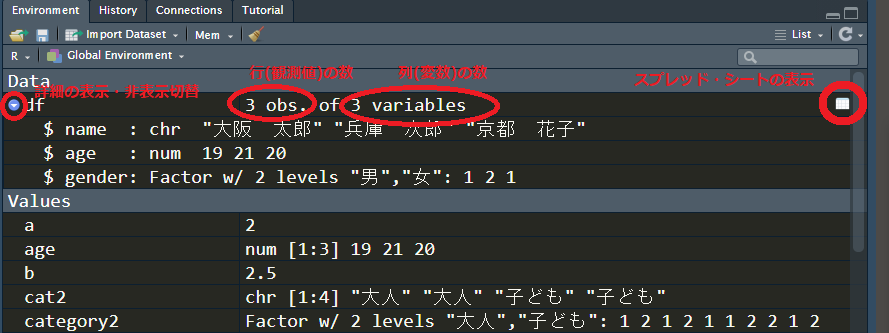
\includegraphics{df1.png}
\caption{データフレーム}
\end{figure}

データフレーム名(いまの場合はdf)もしくはその右にあるスプレッド・シートのマークをクリックすれば,ソースコードのペインにデータフレームがExcelのようなスプレッド・シート形式で表示される。

\begin{figure}
\centering
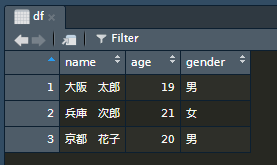
\includegraphics{df2.png}
\caption{データフレーム}
\end{figure}

データフレームに含まれる変数(ベクトル)は,データフレーム名\$ベクトル名で表す。たとえば,dfというデータフレームに含まれるageというベクトル(変数)であれば,df\$ageで表す。

たとえば,3人の平均年齢を求めてみよう。

\begin{Shaded}
\begin{Highlighting}[]
\FunctionTok{mean}\NormalTok{(df}\SpecialCharTok{$}\NormalTok{age)}
\end{Highlighting}
\end{Shaded}

\begin{verbatim}
## [1] 20
\end{verbatim}

\hypertarget{ux30c7ux30fcux30bfux306eux8981ux7d041ux8a18ux8ff0ux7d71ux8a08ux91cf}{%
\chapter{データの要約1(記述統計量)}\label{ux30c7ux30fcux30bfux306eux8981ux7d041ux8a18ux8ff0ux7d71ux8a08ux91cf}}

データを入手したら分析を行う前にデータの概観を把握することが重要である。データフレームにどのような変数が含まれているかを確認し,それぞれの変数の記述統計量(平均値,分位点,分散など)を求め,必要であれば変数間の相関関係を調べよう。

ここでは,Rのパッケージ,tidyverseとstargazerを利用するので読み込んでおく。

\hypertarget{ux30c7ux30fcux30bfux306eux6982ux89b3}{%
\section{データの概観}\label{ux30c7ux30fcux30bfux306eux6982ux89b3}}

ここでは,練習としてRに組み込まれているサンプル・データirisを使ってデータを概観する。まず,サンプル・データをirisというデータフレームに読み込む。

\begin{Shaded}
\begin{Highlighting}[]
\NormalTok{iris }\OtherTok{\textless{}{-}}\NormalTok{ iris}
\end{Highlighting}
\end{Shaded}

irisデータには,150のアヤメについて,種類(3分類),萼片(がくへん)の長さと幅,花弁(かべん)の長さと幅の5つの変数が記録されている。

\begin{longtable}[]{@{}ll@{}}
\toprule
変数名 & 説明 \\
\midrule
\endhead
Sepal.Length & 萼片の長さ \\
Sepal.Width & 萼片の幅 \\
Petal.Length & 花弁の長さ \\
Petal.Width & 花弁の幅 \\
Species & アヤメの種類 \\
\bottomrule
\end{longtable}

データにどのような変数が含まれているかは,スプレッド・シートを表示させれば把握できるが,glimpse()関数を使っても良い(tidyverseの読み込みが必要)。

\begin{Shaded}
\begin{Highlighting}[]
\FunctionTok{glimpse}\NormalTok{(iris)}
\end{Highlighting}
\end{Shaded}

\begin{verbatim}
## Rows: 150
## Columns: 5
## $ Sepal.Length <dbl> 5.1, 4.9, 4.7, 4.6, 5.0, 5.4, 4.6, 5.0, 4.4, 4.9, 5.4, 4.~
## $ Sepal.Width  <dbl> 3.5, 3.0, 3.2, 3.1, 3.6, 3.9, 3.4, 3.4, 2.9, 3.1, 3.7, 3.~
## $ Petal.Length <dbl> 1.4, 1.4, 1.3, 1.5, 1.4, 1.7, 1.4, 1.5, 1.4, 1.5, 1.5, 1.~
## $ Petal.Width  <dbl> 0.2, 0.2, 0.2, 0.2, 0.2, 0.4, 0.3, 0.2, 0.2, 0.1, 0.2, 0.~
## $ Species      <fct> setosa, setosa, setosa, setosa, setosa, setosa, setosa, s~
\end{verbatim}

データの行数(観測数)が150,列数(変数の数)が5であることがわかる。また,5つの変数のはじめのいくつかの観測値を見ることができるので,データのイメージがつかめる。\textless dbl\textgreater や\textless fct\textgreater はそれぞれの変数の型で,dblは実数型,fctはファクター型であることを表している。変数の型には,ほかに文字列型\textless chr\textgreater,整数型\textless int\textgreater などがある。

\hypertarget{ux8981ux7d04ux7d71ux8a08ux8868ux306eux4f5cux6210}{%
\section{要約統計表の作成}\label{ux8981ux7d04ux7d71ux8a08ux8868ux306eux4f5cux6210}}

データ全体のイメージがつかめたら,次は記録されている変数の要約統計量を求めてみよう。summary()関数を用いれば,データフレームに含まれるすべての変数の要約統計量を表示させることができる。

\begin{Shaded}
\begin{Highlighting}[]
\FunctionTok{summary}\NormalTok{(iris)}
\end{Highlighting}
\end{Shaded}

\begin{verbatim}
##   Sepal.Length    Sepal.Width     Petal.Length    Petal.Width   
##  Min.   :4.300   Min.   :2.000   Min.   :1.000   Min.   :0.100  
##  1st Qu.:5.100   1st Qu.:2.800   1st Qu.:1.600   1st Qu.:0.300  
##  Median :5.800   Median :3.000   Median :4.350   Median :1.300  
##  Mean   :5.843   Mean   :3.057   Mean   :3.758   Mean   :1.199  
##  3rd Qu.:6.400   3rd Qu.:3.300   3rd Qu.:5.100   3rd Qu.:1.800  
##  Max.   :7.900   Max.   :4.400   Max.   :6.900   Max.   :2.500  
##        Species  
##  setosa    :50  
##  versicolor:50  
##  virginica :50  
##                 
##                 
## 
\end{verbatim}

数値型の変数については,最小値(Min.),第一四分位(1st Qu.),中央値(Median),平均値(Mean),第三四分位(3rd Qu.),最大値(Max)が表示される。また,ファクター型の変数については,度数分布表が表示される。

これでも十分だが,要約統計量を求める変数や,求める要約統計量を指定したい場合には,summarize()関数を用いる。

\begin{Shaded}
\begin{Highlighting}[]
\FunctionTok{summarize}\NormalTok{(iris, }
\NormalTok{          萼片長平均     }\OtherTok{=} \FunctionTok{mean}\NormalTok{(Sepal.Length),}
\NormalTok{          萼片長標準偏差 }\OtherTok{=} \FunctionTok{sd}\NormalTok{(Sepal.Length),}
\NormalTok{          花弁長平均     }\OtherTok{=} \FunctionTok{mean}\NormalTok{(Petal.Length),}
\NormalTok{          花弁長標準偏差 }\OtherTok{=} \FunctionTok{sd}\NormalTok{(Petal.Length)}
\NormalTok{          )}
\end{Highlighting}
\end{Shaded}

\begin{verbatim}
##   萼片長平均 萼片長標準偏差 花弁長平均 花弁長標準偏差
## 1   5.843333      0.8280661      3.758       1.765298
\end{verbatim}

summarize()関数の第1引数にはデータフレーム名を指定する。第2引数以降は要約統計量の種類と対象の変数名を,名前=関数(変数名)という形式で指定する。名前は表示名なので自由に指定すれば良い。関数の部分には,例として下の表のような関数が利用できる。変数名xには,データフレーム内の変数名を指定すればよく,データフレーム名は必要ない。

\begin{longtable}[]{@{}
  >{\raggedright\arraybackslash}p{(\columnwidth - 2\tabcolsep) * \real{0.5000}}
  >{\raggedright\arraybackslash}p{(\columnwidth - 2\tabcolsep) * \real{0.5000}}@{}}
\toprule
\begin{minipage}[b]{\linewidth}\raggedright
関数
\end{minipage} & \begin{minipage}[b]{\linewidth}\raggedright
説明
\end{minipage} \\
\midrule
\endhead
mean(x) & xの平均値 \\
var(x) & xの分散 \\
sd(x) & xの標準偏差 \\
max(x) & xの最大値 \\
median(x) & xの中央値 \\
min(x) & xの最小値 \\
quantile(x, XX) & xのXX×100パーセンタイル, e.g.~xの25パーセンタイルであればquantile(x,0.25) \\
\bottomrule
\end{longtable}

summarize()関数は,後で述べるようにグループ別の集計のときに役に立つ。

レポートや論文に貼り付けるための要約統計表を作成するには,stargazerパッケージを用いると良い。

\begin{Shaded}
\begin{Highlighting}[]
\FunctionTok{stargazer}\NormalTok{(iris, }\AttributeTok{type =} \StringTok{"text"}\NormalTok{, }\AttributeTok{title=}\StringTok{"要約統計表"}\NormalTok{, }\AttributeTok{digits=}\DecValTok{2}\NormalTok{,}
          \AttributeTok{summary.stat =} \FunctionTok{c}\NormalTok{(}\StringTok{"mean"}\NormalTok{, }\StringTok{"sd"}\NormalTok{, }\StringTok{"min"}\NormalTok{, }\StringTok{"p25"}\NormalTok{, }\StringTok{"median"}\NormalTok{, }\StringTok{"p75"}\NormalTok{, }\StringTok{"max"}\NormalTok{))}
\end{Highlighting}
\end{Shaded}

\begin{verbatim}
## 
## 要約統計表
## =============================================================
## Statistic    Mean St. Dev. Min  Pctl(25) Median Pctl(75) Max 
## -------------------------------------------------------------
## Sepal.Length 5.84   0.83   4.30   5.10    5.80    6.40   7.90
## Sepal.Width  3.06   0.44   2.00   2.80    3.00    3.30   4.40
## Petal.Length 3.76   1.77   1.00   1.60    4.35    5.10   6.90
## Petal.Width  1.20   0.76   0.10   0.30    1.30    1.80   2.50
## -------------------------------------------------------------
\end{verbatim}

stargazer()関数では,第1引数としてデータフレーム(この例ではiris)を指定する。そのほかの引数は必要に応じて指定すれば良い。よく使うオプションだけ説明する。まず,typeは表の出力形式で,``text''(プレーンテキスト),``html'',``latex''のいずれかを指定する。titleは表のタイトル,digitsは表の数値の小数点以下の桁数を指定する。summary.statsは表に含める要約統計量をベクトル形式で指定する。

\begin{longtable}[]{@{}ll@{}}
\toprule
要約統計量 & 指定方法 \\
\midrule
\endhead
平均 & mean \\
標準偏差 & sd \\
最小値 & min \\
最大値 & max \\
XXパーセンタイル(分位点) & pXX \\
\bottomrule
\end{longtable}

\hypertarget{ux76f8ux95a2ux8868}{%
\section{相関表}\label{ux76f8ux95a2ux8868}}

次に,変数間の相関を求めよう。相関表を求めるにはcor()関数を使う。引数にはデータフレーム名を指定する。ただし,irisにファクター型のSpeciesという変数が含まれているため,そのままではエラーになる。そこで,まずデータフレームirisから数値型の4つの変数だけを取り出したデータフレームを作成し,それをcor()関数に指定する。

select()は,データフレームから指定した変数を取り出す関数である。第1引数には取り出したい変数が含まれるデータフレームを指定する。第2引数以降は取り出したい変数名をカンマで区切って指定する。たとえば,select(dataframe,a,b)はdataframe\$aとdataframe\$bの2つの変数が含まれるデータフレームとなる。逆にデータフレームから指定した変数を除外したいときには,第2変数以降に変数名に''-``をつけて指定する。たとえば,select(dataframe,-a)はdataframeから変数aを除いたデータフレームとなる。また,変数は列番号で指定することも可能である。たとえば,select(dataframe,2:4)はdataframeから2列目から4列目までの変数を取り出したデータフレームとなる。

irisでは,5つの変数のうち数値型の4つを取り出して相関表を作成したいので,ファクター型の変数Speciesだけを除外してcor()関数に指定すれば良い。

\begin{Shaded}
\begin{Highlighting}[]
\FunctionTok{cor}\NormalTok{(}\FunctionTok{select}\NormalTok{(iris,}\SpecialCharTok{{-}}\NormalTok{Species))}
\end{Highlighting}
\end{Shaded}

\begin{verbatim}
##              Sepal.Length Sepal.Width Petal.Length Petal.Width
## Sepal.Length    1.0000000  -0.1175698    0.8717538   0.8179411
## Sepal.Width    -0.1175698   1.0000000   -0.4284401  -0.3661259
## Petal.Length    0.8717538  -0.4284401    1.0000000   0.9628654
## Petal.Width     0.8179411  -0.3661259    0.9628654   1.0000000
\end{verbatim}

以下のコードでも同じ結果が得られる。

\begin{Shaded}
\begin{Highlighting}[]
\FunctionTok{cor}\NormalTok{(}\FunctionTok{select}\NormalTok{(iris,}\DecValTok{1}\SpecialCharTok{:}\DecValTok{4}\NormalTok{))}
\FunctionTok{cor}\NormalTok{(}\FunctionTok{select}\NormalTok{(iris, Sepal.Length, Sepal.Width, Petal.Length, Petal.Width)}
\end{Highlighting}
\end{Shaded}

\hypertarget{ux30b0ux30ebux30fcux30d7ux5206ux3051}{%
\section{グループ分け}\label{ux30b0ux30ebux30fcux30d7ux5206ux3051}}

データをグループに分けて,グループごとに要約統計を求めてみよう。irisデータでは,アヤメはsetosa,versicolor,virginicaの3種類に分類されている。アヤメの種類ごとに萼片と花弁の長さ,幅の平均を求めてみよう。そのための方法はいくつか考えられる。

\hypertarget{ux30c7ux30fcux30bfux30d5ux30ecux30fcux30e0ux3092ux5206ux5272ux3059ux308b}{%
\subsection{データフレームを分割する}\label{ux30c7ux30fcux30bfux30d5ux30ecux30fcux30e0ux3092ux5206ux5272ux3059ux308b}}

まず,データフレームをアヤメの種類ごとに分割する方法である。filter()はデータフレームから条件を満たすデータ(行)を取り出す関数である。

\begin{Shaded}
\begin{Highlighting}[]
\NormalTok{iris\_setosa }\OtherTok{\textless{}{-}} \FunctionTok{filter}\NormalTok{(iris, Species}\SpecialCharTok{==}\StringTok{"setosa"}\NormalTok{)}
\NormalTok{iris\_versicolor }\OtherTok{\textless{}{-}} \FunctionTok{filter}\NormalTok{(iris, Species}\SpecialCharTok{==}\StringTok{"versicolor"}\NormalTok{)}
\NormalTok{iris\_virginica }\OtherTok{\textless{}{-}} \FunctionTok{filter}\NormalTok{(iris, Species}\SpecialCharTok{==}\StringTok{"virginica"}\NormalTok{)}
\end{Highlighting}
\end{Shaded}

アヤメの種類ごとのデータフレームができるので,それぞれのデータフレームで要約統計表を作成する。

\begin{Shaded}
\begin{Highlighting}[]
\FunctionTok{stargazer}\NormalTok{(iris\_setosa, }\AttributeTok{type =} \StringTok{"text"}\NormalTok{, }\AttributeTok{title=}\StringTok{"setosa"}\NormalTok{, }\AttributeTok{digits=}\DecValTok{2}\NormalTok{,}
          \AttributeTok{summary.stat =} \FunctionTok{c}\NormalTok{(}\StringTok{"mean"}\NormalTok{, }\StringTok{"sd"}\NormalTok{, }\StringTok{"min"}\NormalTok{, }\StringTok{"p25"}\NormalTok{, }\StringTok{"median"}\NormalTok{, }\StringTok{"p75"}\NormalTok{, }\StringTok{"max"}\NormalTok{))}
\end{Highlighting}
\end{Shaded}

\begin{verbatim}
## 
## setosa
## =============================================================
## Statistic    Mean St. Dev. Min  Pctl(25) Median Pctl(75) Max 
## -------------------------------------------------------------
## Sepal.Length 5.01   0.35   4.30   4.80    5.00    5.20   5.80
## Sepal.Width  3.43   0.38   2.30   3.20    3.40    3.68   4.40
## Petal.Length 1.46   0.17   1.00   1.40    1.50    1.58   1.90
## Petal.Width  0.25   0.11   0.10   0.20    0.20    0.30   0.60
## -------------------------------------------------------------
\end{verbatim}

\begin{Shaded}
\begin{Highlighting}[]
\FunctionTok{stargazer}\NormalTok{(iris\_versicolor, }\AttributeTok{type =} \StringTok{"text"}\NormalTok{, }\AttributeTok{title=}\StringTok{"versicolor"}\NormalTok{, }\AttributeTok{digits=}\DecValTok{2}\NormalTok{,}
          \AttributeTok{summary.stat =} \FunctionTok{c}\NormalTok{(}\StringTok{"mean"}\NormalTok{, }\StringTok{"sd"}\NormalTok{, }\StringTok{"min"}\NormalTok{, }\StringTok{"p25"}\NormalTok{, }\StringTok{"median"}\NormalTok{, }\StringTok{"p75"}\NormalTok{, }\StringTok{"max"}\NormalTok{))}
\end{Highlighting}
\end{Shaded}

\begin{verbatim}
## 
## versicolor
## =============================================================
## Statistic    Mean St. Dev. Min  Pctl(25) Median Pctl(75) Max 
## -------------------------------------------------------------
## Sepal.Length 5.94   0.52   4.90   5.60    5.90    6.30   7.00
## Sepal.Width  2.77   0.31   2.00   2.52    2.80    3.00   3.40
## Petal.Length 4.26   0.47   3.00   4.00    4.35    4.60   5.10
## Petal.Width  1.33   0.20   1.00   1.20    1.30    1.50   1.80
## -------------------------------------------------------------
\end{verbatim}

\begin{Shaded}
\begin{Highlighting}[]
\FunctionTok{stargazer}\NormalTok{(iris\_virginica, }\AttributeTok{type =} \StringTok{"text"}\NormalTok{, }\AttributeTok{title=}\StringTok{"virginica"}\NormalTok{, }\AttributeTok{digits=}\DecValTok{2}\NormalTok{,}
          \AttributeTok{summary.stat =} \FunctionTok{c}\NormalTok{(}\StringTok{"mean"}\NormalTok{, }\StringTok{"sd"}\NormalTok{, }\StringTok{"min"}\NormalTok{, }\StringTok{"p25"}\NormalTok{, }\StringTok{"median"}\NormalTok{, }\StringTok{"p75"}\NormalTok{, }\StringTok{"max"}\NormalTok{))}
\end{Highlighting}
\end{Shaded}

\begin{verbatim}
## 
## virginica
## =============================================================
## Statistic    Mean St. Dev. Min  Pctl(25) Median Pctl(75) Max 
## -------------------------------------------------------------
## Sepal.Length 6.59   0.64   4.90   6.23    6.50    6.90   7.90
## Sepal.Width  2.97   0.32   2.20   2.80    3.00    3.18   3.80
## Petal.Length 5.55   0.55   4.50   5.10    5.55    5.88   6.90
## Petal.Width  2.03   0.27   1.40   1.80    2.00    2.30   2.50
## -------------------------------------------------------------
\end{verbatim}

\hypertarget{group_byux3092ux4f7fux3046}{%
\subsection{group\_by()を使う}\label{group_byux3092ux4f7fux3046}}

group\_by関数を使うと,グループに分類されたデータフレームを作成することができる。第1引数には分類したいデータフレーム名,第2引数以降は分類を行うためのファクター型変数を指定する。複数のファクター型変数を指定して,階層的な分類を行うことも可能。グループに分類されたデータフレームにsummarize()関数を適用すると,グループごとの要約統計量が計算される。

\begin{Shaded}
\begin{Highlighting}[]
\NormalTok{iris\_grouped }\OtherTok{\textless{}{-}} \FunctionTok{group\_by}\NormalTok{(iris, Species)}

\FunctionTok{summarize}\NormalTok{(iris\_grouped, }
\NormalTok{          萼片長平均     }\OtherTok{=} \FunctionTok{mean}\NormalTok{(Sepal.Length),}
\NormalTok{          萼片長標準偏差 }\OtherTok{=} \FunctionTok{sd}\NormalTok{(Sepal.Length),}
\NormalTok{          花弁長平均     }\OtherTok{=} \FunctionTok{mean}\NormalTok{(Petal.Length),}
\NormalTok{          花弁長標準偏差 }\OtherTok{=} \FunctionTok{sd}\NormalTok{(Petal.Length)}
\NormalTok{          )}
\end{Highlighting}
\end{Shaded}

\begin{verbatim}
## # A tibble: 3 x 5
##   Species    萼片長平均 萼片長標準偏差 花弁長平均 花弁長標準偏差
##   <fct>           <dbl>          <dbl>      <dbl>          <dbl>
## 1 setosa           5.01          0.352       1.46          0.174
## 2 versicolor       5.94          0.516       4.26          0.470
## 3 virginica        6.59          0.636       5.55          0.552
\end{verbatim}

\hypertarget{xtabsux3092ux4f7fux3046}{%
\subsection{xtabs()を使う}\label{xtabsux3092ux4f7fux3046}}

xtabs()関数を使うと,多次元分割表を柔軟に作成することができる。第1引数には形式を,第2引数にはデータフレーム名を指定する。形式は,\texttt{\textasciitilde{}x1+x2+...}か\texttt{y\textasciitilde{}x1+x2+...}の形で指定する。たとえば,\texttt{\textasciitilde{}x1+x2}を指定すれば,x1,x2で表を分割し,各セルに入るデータ数が得られる。\texttt{y\textasciitilde{}x1+x2}を指定すれば,x1,x2で表を分割し,各セルに入るデータのyの合計が得られる。

irisでは分類に用いることができる変数はSpeciesの1つしかないが,それでもxtabs()を適用できる。以下のコードでSpeciesごとのデータ数の表を作成できる。

\begin{Shaded}
\begin{Highlighting}[]
\FunctionTok{xtabs}\NormalTok{(}\SpecialCharTok{\textasciitilde{}}\NormalTok{Species,iris)}
\end{Highlighting}
\end{Shaded}

\begin{verbatim}
## Species
##     setosa versicolor  virginica 
##         50         50         50
\end{verbatim}

次に,以下のコードでSpeciesごとの萼片長の合計値の表を作成できる。

\begin{Shaded}
\begin{Highlighting}[]
\FunctionTok{xtabs}\NormalTok{(Sepal.Length}\SpecialCharTok{\textasciitilde{}}\NormalTok{Species,iris)}
\end{Highlighting}
\end{Shaded}

\begin{verbatim}
## Species
##     setosa versicolor  virginica 
##      250.3      296.8      329.4
\end{verbatim}

平均値は合計値をデータ数で割ったものなので,Speciesごとの萼片長の平均値を以下のように求められる。

\begin{Shaded}
\begin{Highlighting}[]
\FunctionTok{xtabs}\NormalTok{(Sepal.Length}\SpecialCharTok{\textasciitilde{}}\NormalTok{Species,iris)}\SpecialCharTok{/}\FunctionTok{xtabs}\NormalTok{(}\SpecialCharTok{\textasciitilde{}}\NormalTok{Species,iris)}
\end{Highlighting}
\end{Shaded}

\begin{verbatim}
## Species
##     setosa versicolor  virginica 
##      5.006      5.936      6.588
\end{verbatim}

\hypertarget{ux30c7ux30fcux30bfux306eux8981ux7d042ux30b0ux30e9ux30d5ux306eux4f5cux6210}{%
\chapter{データの要約2(グラフの作成)}\label{ux30c7ux30fcux30bfux306eux8981ux7d042ux30b0ux30e9ux30d5ux306eux4f5cux6210}}

データを概観するためには,記述統計量を求めるとともに,グラフを作成して視覚的にデータの特性を捉えることも重要である。一変数の分布を概観するにはヒストグラム,変数間の関係を概観するには散布図を描いてみるのが有効。

R本体でもさまざまなグラフを作成することができるが,ggplot2というパッケージを用いればより簡単にモダンなグラフを作成することができる。ggplot2は,tidyverseに含まれているので,tidyverseを読み込んでおく。

\begin{Shaded}
\begin{Highlighting}[]
\FunctionTok{library}\NormalTok{(tidyverse)}
\end{Highlighting}
\end{Shaded}

また,練習用データとしてirisを用いる。

\begin{Shaded}
\begin{Highlighting}[]
\NormalTok{iris }\OtherTok{\textless{}{-}}\NormalTok{ iris}
\end{Highlighting}
\end{Shaded}

\hypertarget{ux30d2ux30b9ux30c8ux30b0ux30e9ux30e0}{%
\section{ヒストグラム}\label{ux30d2ux30b9ux30c8ux30b0ux30e9ux30e0}}

まず,150のアヤメの萼片の長さについて,ヒストグラムを作成してみよう。

ggplot2でグラフを作成するには,まずグラフ・オブジェクトを作成する。

\begin{Shaded}
\begin{Highlighting}[]
\NormalTok{g }\OtherTok{\textless{}{-}}\NormalTok{ iris }\SpecialCharTok{\%\textgreater{}\%} 
  \FunctionTok{ggplot}\NormalTok{(}\FunctionTok{aes}\NormalTok{(}\AttributeTok{x=}\NormalTok{Sepal.Length))}
\end{Highlighting}
\end{Shaded}

ここでは,gというオブジェクトにグラフの素地を作成している。ggplot()関数の振舞いを理解するのは簡単ではないが,まずは決まったやり方を覚えよう。ggplot()関数を使うときには,まずデータフレームとx軸,y軸にとる変数などをaes()で指定しグラフの素地を作成する。ここではggplot()関数にパイプでデータフレームirisを渡し,aes()でグラフのx軸に用いる変数Sepal.Lengthを指定している。ヒストグラムの場合に最低限必要なのは,x軸の変数(ヒストグラムを作成する変数)だけである。

次にヒストグラムを追加する。

\begin{Shaded}
\begin{Highlighting}[]
\NormalTok{g }\OtherTok{\textless{}{-}}\NormalTok{ g}\SpecialCharTok{+}\FunctionTok{geom\_histogram}\NormalTok{()}
\end{Highlighting}
\end{Shaded}

このように,ggplotでは作成した素地に,グラフやさまざまなパーツを足していくことで,好みのグラフを作成する。

グラフを表示させるにはplot()関数を用いる。

\begin{Shaded}
\begin{Highlighting}[]
\FunctionTok{plot}\NormalTok{(g)}
\end{Highlighting}
\end{Shaded}

\begin{verbatim}
## `stat_bin()` using `bins = 30`. Pick better value with `binwidth`.
\end{verbatim}

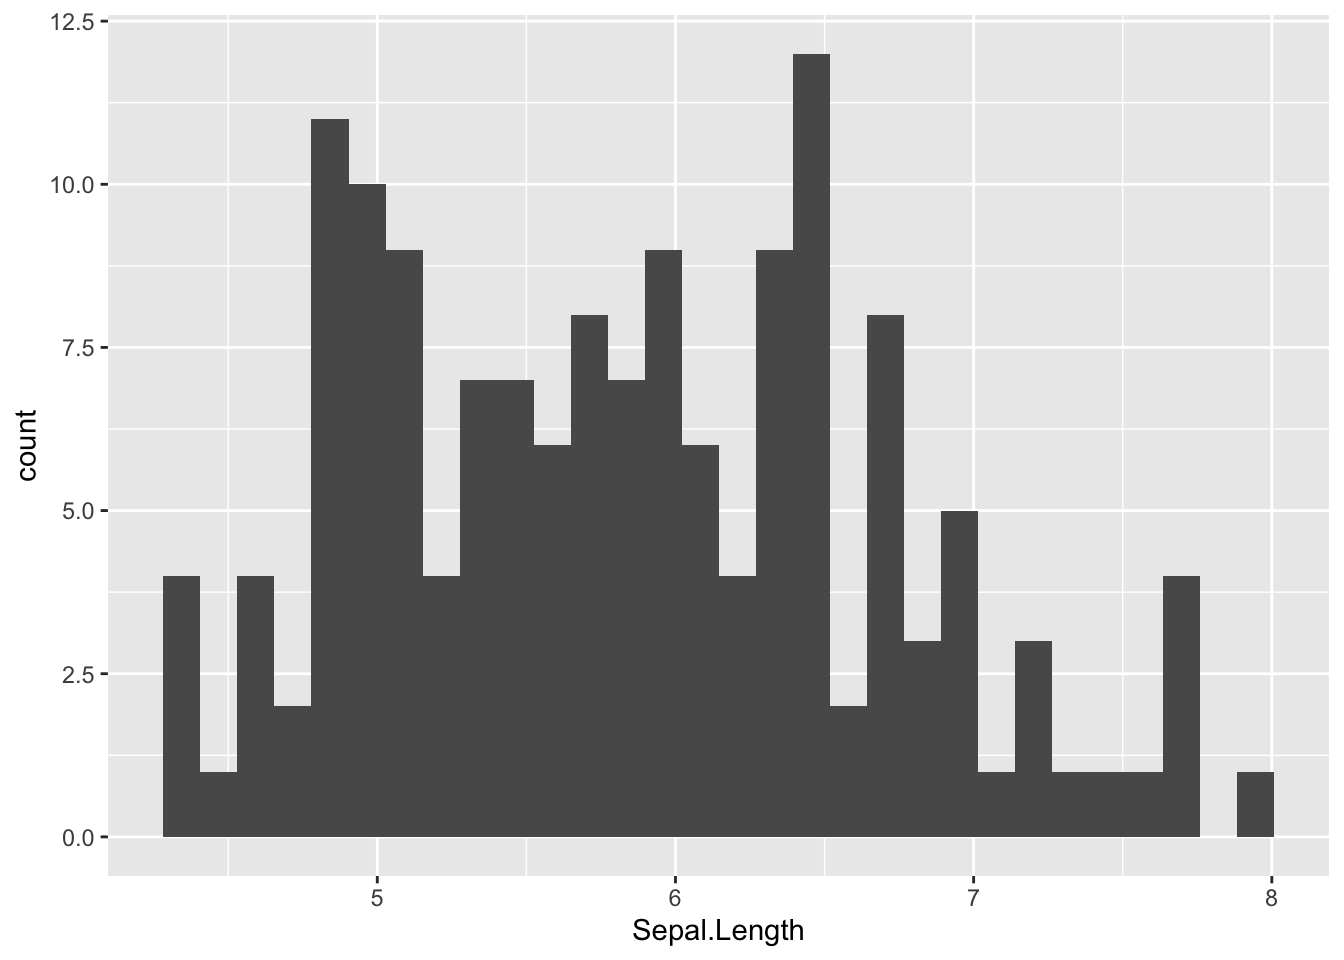
\includegraphics{_main_files/figure-latex/unnamed-chunk-38-1.pdf}

とくに何も指定しなくても,Rが適当に区間を分割してヒストグラムを描いてくれる。

このままだと見にくいので,ヒストグラムのビンの幅を変更し,枠線や塗り色を指定してみよう。ヒストグラムの細かい設定は,geom\_histogram()の引数に指定すれば良い。

\begin{Shaded}
\begin{Highlighting}[]
\NormalTok{g }\OtherTok{\textless{}{-}}\NormalTok{ iris }\SpecialCharTok{\%\textgreater{}\%} 
  \FunctionTok{ggplot}\NormalTok{(}\FunctionTok{aes}\NormalTok{(}\AttributeTok{x=}\NormalTok{Sepal.Length))}\SpecialCharTok{+}
  \FunctionTok{geom\_histogram}\NormalTok{(}\AttributeTok{binwidth=}\FloatTok{0.25}\NormalTok{,}\AttributeTok{color=}\StringTok{"black"}\NormalTok{, }\AttributeTok{fill=}\StringTok{"blue"}\NormalTok{)}

\FunctionTok{plot}\NormalTok{(g)}
\end{Highlighting}
\end{Shaded}

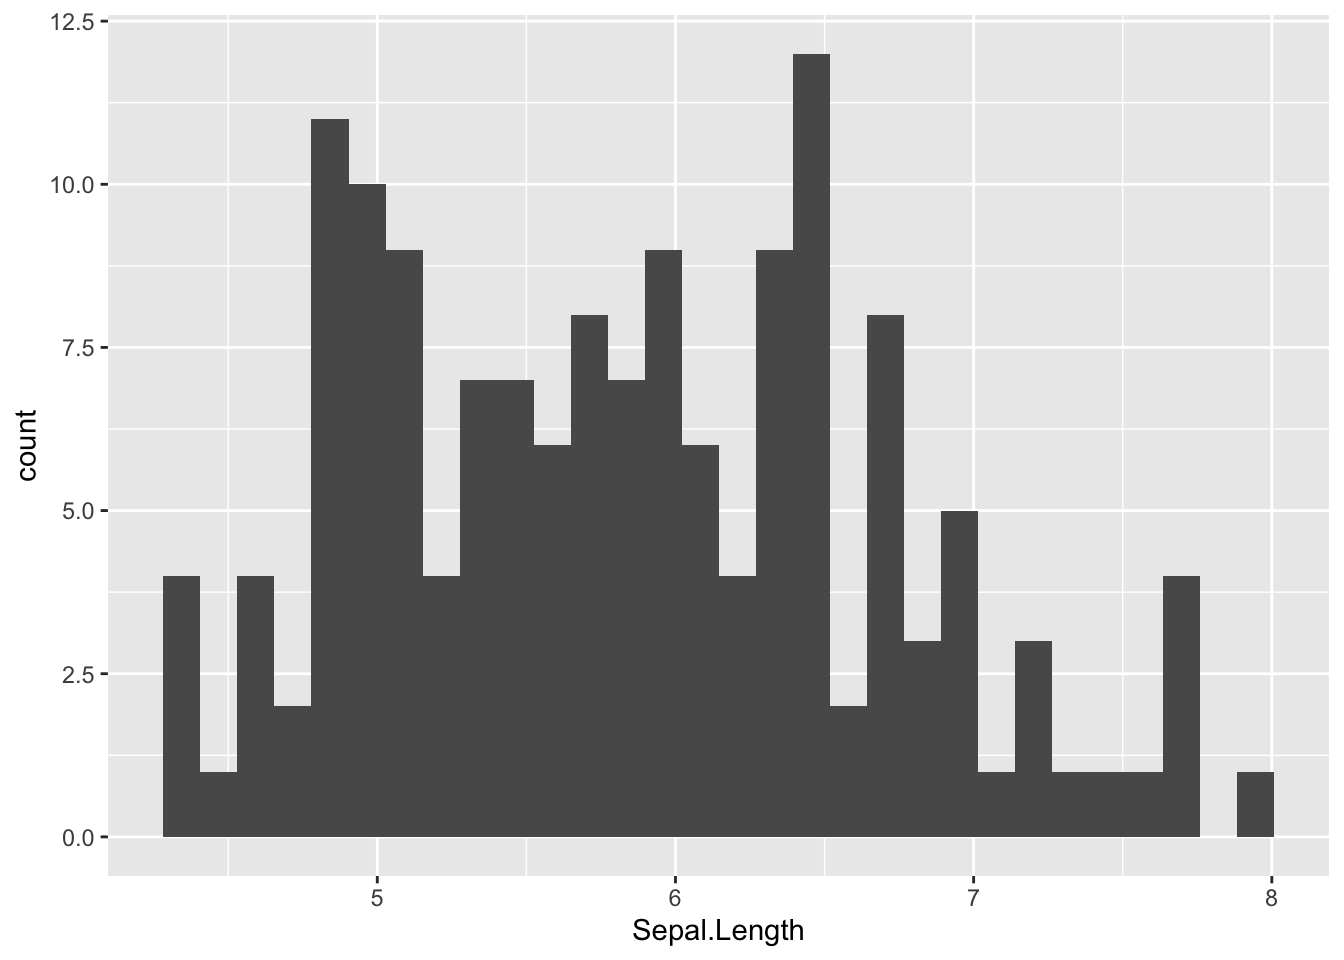
\includegraphics{_main_files/figure-latex/unnamed-chunk-39-1.pdf}

次に,グラフの軸のラベルを変更して,グラフ・タイトルをつけてみよう。下のように,グラフ・オブジェクトにlabs()で軸ラベルやタイトルの設定を足す。

\begin{Shaded}
\begin{Highlighting}[]
\NormalTok{g }\OtherTok{\textless{}{-}}\NormalTok{ iris }\SpecialCharTok{\%\textgreater{}\%} 
  \FunctionTok{ggplot}\NormalTok{(}\FunctionTok{aes}\NormalTok{(}\AttributeTok{x=}\NormalTok{Sepal.Length))}\SpecialCharTok{+}
  \FunctionTok{geom\_histogram}\NormalTok{(}\AttributeTok{binwidth=}\FloatTok{0.25}\NormalTok{,}\AttributeTok{color=}\StringTok{"black"}\NormalTok{, }\AttributeTok{fill=}\StringTok{"blue"}\NormalTok{)}\SpecialCharTok{+}
  \FunctionTok{labs}\NormalTok{(}\AttributeTok{x =} \StringTok{"萼片長"}\NormalTok{, }\AttributeTok{y =} \StringTok{"頻度"}\NormalTok{, }\AttributeTok{title =} \StringTok{"アヤメの萼片長の分布"}\NormalTok{)}

\FunctionTok{plot}\NormalTok{(g)}
\end{Highlighting}
\end{Shaded}

\begin{verbatim}
## Warning in grid.Call(C_textBounds, as.graphicsAnnot(x$label), x$x, x$y, :
## 'mbcsToSbcs' 中の '頻度' で変換に失敗: <e9> をドットで置き換えました
\end{verbatim}

\begin{verbatim}
## Warning in grid.Call(C_textBounds, as.graphicsAnnot(x$label), x$x, x$y, :
## 'mbcsToSbcs' 中の '頻度' で変換に失敗: <a0> をドットで置き換えました
\end{verbatim}

\begin{verbatim}
## Warning in grid.Call(C_textBounds, as.graphicsAnnot(x$label), x$x, x$y, :
## 'mbcsToSbcs' 中の '頻度' で変換に失敗: <bb> をドットで置き換えました
\end{verbatim}

\begin{verbatim}
## Warning in grid.Call(C_textBounds, as.graphicsAnnot(x$label), x$x, x$y, :
## 'mbcsToSbcs' 中の '頻度' で変換に失敗: <e5> をドットで置き換えました
\end{verbatim}

\begin{verbatim}
## Warning in grid.Call(C_textBounds, as.graphicsAnnot(x$label), x$x, x$y, :
## 'mbcsToSbcs' 中の '頻度' で変換に失敗: <ba> をドットで置き換えました
\end{verbatim}

\begin{verbatim}
## Warning in grid.Call(C_textBounds, as.graphicsAnnot(x$label), x$x, x$y, :
## 'mbcsToSbcs' 中の '頻度' で変換に失敗: <a6> をドットで置き換えました
\end{verbatim}

\begin{verbatim}
## Warning in grid.Call(C_textBounds, as.graphicsAnnot(x$label), x$x, x$y, :
## 'mbcsToSbcs' 中の '頻度' で変換に失敗: <e9> をドットで置き換えました
\end{verbatim}

\begin{verbatim}
## Warning in grid.Call(C_textBounds, as.graphicsAnnot(x$label), x$x, x$y, :
## 'mbcsToSbcs' 中の '頻度' で変換に失敗: <a0> をドットで置き換えました
\end{verbatim}

\begin{verbatim}
## Warning in grid.Call(C_textBounds, as.graphicsAnnot(x$label), x$x, x$y, :
## 'mbcsToSbcs' 中の '頻度' で変換に失敗: <bb> をドットで置き換えました
\end{verbatim}

\begin{verbatim}
## Warning in grid.Call(C_textBounds, as.graphicsAnnot(x$label), x$x, x$y, :
## 'mbcsToSbcs' 中の '頻度' で変換に失敗: <e5> をドットで置き換えました
\end{verbatim}

\begin{verbatim}
## Warning in grid.Call(C_textBounds, as.graphicsAnnot(x$label), x$x, x$y, :
## 'mbcsToSbcs' 中の '頻度' で変換に失敗: <ba> をドットで置き換えました
\end{verbatim}

\begin{verbatim}
## Warning in grid.Call(C_textBounds, as.graphicsAnnot(x$label), x$x, x$y, :
## 'mbcsToSbcs' 中の '頻度' で変換に失敗: <a6> をドットで置き換えました
\end{verbatim}

\begin{verbatim}
## Warning in grid.Call(C_textBounds, as.graphicsAnnot(x$label), x$x, x$y, :
## 'mbcsToSbcs' 中の 'アヤメの萼片長の分布' で変換に失敗: <e3> をドットで置き換えま
## した
\end{verbatim}

\begin{verbatim}
## Warning in grid.Call(C_textBounds, as.graphicsAnnot(x$label), x$x, x$y, :
## 'mbcsToSbcs' 中の 'アヤメの萼片長の分布' で変換に失敗: <82> をドットで置き換えま
## した
\end{verbatim}

\begin{verbatim}
## Warning in grid.Call(C_textBounds, as.graphicsAnnot(x$label), x$x, x$y, :
## 'mbcsToSbcs' 中の 'アヤメの萼片長の分布' で変換に失敗: <a2> をドットで置き換えま
## した
\end{verbatim}

\begin{verbatim}
## Warning in grid.Call(C_textBounds, as.graphicsAnnot(x$label), x$x, x$y, :
## 'mbcsToSbcs' 中の 'アヤメの萼片長の分布' で変換に失敗: <e3> をドットで置き換えま
## した
\end{verbatim}

\begin{verbatim}
## Warning in grid.Call(C_textBounds, as.graphicsAnnot(x$label), x$x, x$y, :
## 'mbcsToSbcs' 中の 'アヤメの萼片長の分布' で変換に失敗: <83> をドットで置き換えま
## した
\end{verbatim}

\begin{verbatim}
## Warning in grid.Call(C_textBounds, as.graphicsAnnot(x$label), x$x, x$y, :
## 'mbcsToSbcs' 中の 'アヤメの萼片長の分布' で変換に失敗: <a4> をドットで置き換えま
## した
\end{verbatim}

\begin{verbatim}
## Warning in grid.Call(C_textBounds, as.graphicsAnnot(x$label), x$x, x$y, :
## 'mbcsToSbcs' 中の 'アヤメの萼片長の分布' で変換に失敗: <e3> をドットで置き換えま
## した
\end{verbatim}

\begin{verbatim}
## Warning in grid.Call(C_textBounds, as.graphicsAnnot(x$label), x$x, x$y, :
## 'mbcsToSbcs' 中の 'アヤメの萼片長の分布' で変換に失敗: <83> をドットで置き換えま
## した
\end{verbatim}

\begin{verbatim}
## Warning in grid.Call(C_textBounds, as.graphicsAnnot(x$label), x$x, x$y, :
## 'mbcsToSbcs' 中の 'アヤメの萼片長の分布' で変換に失敗: <a1> をドットで置き換えま
## した
\end{verbatim}

\begin{verbatim}
## Warning in grid.Call(C_textBounds, as.graphicsAnnot(x$label), x$x, x$y, :
## 'mbcsToSbcs' 中の 'アヤメの萼片長の分布' で変換に失敗: <e3> をドットで置き換えま
## した
\end{verbatim}

\begin{verbatim}
## Warning in grid.Call(C_textBounds, as.graphicsAnnot(x$label), x$x, x$y, :
## 'mbcsToSbcs' 中の 'アヤメの萼片長の分布' で変換に失敗: <81> をドットで置き換えま
## した
\end{verbatim}

\begin{verbatim}
## Warning in grid.Call(C_textBounds, as.graphicsAnnot(x$label), x$x, x$y, :
## 'mbcsToSbcs' 中の 'アヤメの萼片長の分布' で変換に失敗: <ae> をドットで置き換えま
## した
\end{verbatim}

\begin{verbatim}
## Warning in grid.Call(C_textBounds, as.graphicsAnnot(x$label), x$x, x$y, :
## 'mbcsToSbcs' 中の 'アヤメの萼片長の分布' で変換に失敗: <e8> をドットで置き換えま
## した
\end{verbatim}

\begin{verbatim}
## Warning in grid.Call(C_textBounds, as.graphicsAnnot(x$label), x$x, x$y, :
## 'mbcsToSbcs' 中の 'アヤメの萼片長の分布' で変換に失敗: <90> をドットで置き換えま
## した
\end{verbatim}

\begin{verbatim}
## Warning in grid.Call(C_textBounds, as.graphicsAnnot(x$label), x$x, x$y, :
## 'mbcsToSbcs' 中の 'アヤメの萼片長の分布' で変換に失敗: <bc> をドットで置き換えま
## した
\end{verbatim}

\begin{verbatim}
## Warning in grid.Call(C_textBounds, as.graphicsAnnot(x$label), x$x, x$y, :
## 'mbcsToSbcs' 中の 'アヤメの萼片長の分布' で変換に失敗: <e7> をドットで置き換えま
## した
\end{verbatim}

\begin{verbatim}
## Warning in grid.Call(C_textBounds, as.graphicsAnnot(x$label), x$x, x$y, :
## 'mbcsToSbcs' 中の 'アヤメの萼片長の分布' で変換に失敗: <89> をドットで置き換えま
## した
\end{verbatim}

\begin{verbatim}
## Warning in grid.Call(C_textBounds, as.graphicsAnnot(x$label), x$x, x$y, :
## 'mbcsToSbcs' 中の 'アヤメの萼片長の分布' で変換に失敗: <87> をドットで置き換えま
## した
\end{verbatim}

\begin{verbatim}
## Warning in grid.Call(C_textBounds, as.graphicsAnnot(x$label), x$x, x$y, :
## 'mbcsToSbcs' 中の 'アヤメの萼片長の分布' で変換に失敗: <e9> をドットで置き換えま
## した
\end{verbatim}

\begin{verbatim}
## Warning in grid.Call(C_textBounds, as.graphicsAnnot(x$label), x$x, x$y, :
## 'mbcsToSbcs' 中の 'アヤメの萼片長の分布' で変換に失敗: <95> をドットで置き換えま
## した
\end{verbatim}

\begin{verbatim}
## Warning in grid.Call(C_textBounds, as.graphicsAnnot(x$label), x$x, x$y, :
## 'mbcsToSbcs' 中の 'アヤメの萼片長の分布' で変換に失敗: <b7> をドットで置き換えま
## した
\end{verbatim}

\begin{verbatim}
## Warning in grid.Call(C_textBounds, as.graphicsAnnot(x$label), x$x, x$y, :
## 'mbcsToSbcs' 中の 'アヤメの萼片長の分布' で変換に失敗: <e3> をドットで置き換えま
## した
\end{verbatim}

\begin{verbatim}
## Warning in grid.Call(C_textBounds, as.graphicsAnnot(x$label), x$x, x$y, :
## 'mbcsToSbcs' 中の 'アヤメの萼片長の分布' で変換に失敗: <81> をドットで置き換えま
## した
\end{verbatim}

\begin{verbatim}
## Warning in grid.Call(C_textBounds, as.graphicsAnnot(x$label), x$x, x$y, :
## 'mbcsToSbcs' 中の 'アヤメの萼片長の分布' で変換に失敗: <ae> をドットで置き換えま
## した
\end{verbatim}

\begin{verbatim}
## Warning in grid.Call(C_textBounds, as.graphicsAnnot(x$label), x$x, x$y, :
## 'mbcsToSbcs' 中の 'アヤメの萼片長の分布' で変換に失敗: <e5> をドットで置き換えま
## した
\end{verbatim}

\begin{verbatim}
## Warning in grid.Call(C_textBounds, as.graphicsAnnot(x$label), x$x, x$y, :
## 'mbcsToSbcs' 中の 'アヤメの萼片長の分布' で変換に失敗: <88> をドットで置き換えま
## した
\end{verbatim}

\begin{verbatim}
## Warning in grid.Call(C_textBounds, as.graphicsAnnot(x$label), x$x, x$y, :
## 'mbcsToSbcs' 中の 'アヤメの萼片長の分布' で変換に失敗: <86> をドットで置き換えま
## した
\end{verbatim}

\begin{verbatim}
## Warning in grid.Call(C_textBounds, as.graphicsAnnot(x$label), x$x, x$y, :
## 'mbcsToSbcs' 中の 'アヤメの萼片長の分布' で変換に失敗: <e5> をドットで置き換えま
## した
\end{verbatim}

\begin{verbatim}
## Warning in grid.Call(C_textBounds, as.graphicsAnnot(x$label), x$x, x$y, :
## 'mbcsToSbcs' 中の 'アヤメの萼片長の分布' で変換に失敗: <b8> をドットで置き換えま
## した
\end{verbatim}

\begin{verbatim}
## Warning in grid.Call(C_textBounds, as.graphicsAnnot(x$label), x$x, x$y, :
## 'mbcsToSbcs' 中の 'アヤメの萼片長の分布' で変換に失敗: <83> をドットで置き換えま
## した
\end{verbatim}

\begin{verbatim}
## Warning in grid.Call(C_textBounds, as.graphicsAnnot(x$label), x$x, x$y, :
## 'mbcsToSbcs' 中の 'アヤメの萼片長の分布' で変換に失敗: <e3> をドットで置き換えま
## した
\end{verbatim}

\begin{verbatim}
## Warning in grid.Call(C_textBounds, as.graphicsAnnot(x$label), x$x, x$y, :
## 'mbcsToSbcs' 中の 'アヤメの萼片長の分布' で変換に失敗: <82> をドットで置き換えま
## した
\end{verbatim}

\begin{verbatim}
## Warning in grid.Call(C_textBounds, as.graphicsAnnot(x$label), x$x, x$y, :
## 'mbcsToSbcs' 中の 'アヤメの萼片長の分布' で変換に失敗: <a2> をドットで置き換えま
## した
\end{verbatim}

\begin{verbatim}
## Warning in grid.Call(C_textBounds, as.graphicsAnnot(x$label), x$x, x$y, :
## 'mbcsToSbcs' 中の 'アヤメの萼片長の分布' で変換に失敗: <e3> をドットで置き換えま
## した
\end{verbatim}

\begin{verbatim}
## Warning in grid.Call(C_textBounds, as.graphicsAnnot(x$label), x$x, x$y, :
## 'mbcsToSbcs' 中の 'アヤメの萼片長の分布' で変換に失敗: <83> をドットで置き換えま
## した
\end{verbatim}

\begin{verbatim}
## Warning in grid.Call(C_textBounds, as.graphicsAnnot(x$label), x$x, x$y, :
## 'mbcsToSbcs' 中の 'アヤメの萼片長の分布' で変換に失敗: <a4> をドットで置き換えま
## した
\end{verbatim}

\begin{verbatim}
## Warning in grid.Call(C_textBounds, as.graphicsAnnot(x$label), x$x, x$y, :
## 'mbcsToSbcs' 中の 'アヤメの萼片長の分布' で変換に失敗: <e3> をドットで置き換えま
## した
\end{verbatim}

\begin{verbatim}
## Warning in grid.Call(C_textBounds, as.graphicsAnnot(x$label), x$x, x$y, :
## 'mbcsToSbcs' 中の 'アヤメの萼片長の分布' で変換に失敗: <83> をドットで置き換えま
## した
\end{verbatim}

\begin{verbatim}
## Warning in grid.Call(C_textBounds, as.graphicsAnnot(x$label), x$x, x$y, :
## 'mbcsToSbcs' 中の 'アヤメの萼片長の分布' で変換に失敗: <a1> をドットで置き換えま
## した
\end{verbatim}

\begin{verbatim}
## Warning in grid.Call(C_textBounds, as.graphicsAnnot(x$label), x$x, x$y, :
## 'mbcsToSbcs' 中の 'アヤメの萼片長の分布' で変換に失敗: <e3> をドットで置き換えま
## した
\end{verbatim}

\begin{verbatim}
## Warning in grid.Call(C_textBounds, as.graphicsAnnot(x$label), x$x, x$y, :
## 'mbcsToSbcs' 中の 'アヤメの萼片長の分布' で変換に失敗: <81> をドットで置き換えま
## した
\end{verbatim}

\begin{verbatim}
## Warning in grid.Call(C_textBounds, as.graphicsAnnot(x$label), x$x, x$y, :
## 'mbcsToSbcs' 中の 'アヤメの萼片長の分布' で変換に失敗: <ae> をドットで置き換えま
## した
\end{verbatim}

\begin{verbatim}
## Warning in grid.Call(C_textBounds, as.graphicsAnnot(x$label), x$x, x$y, :
## 'mbcsToSbcs' 中の 'アヤメの萼片長の分布' で変換に失敗: <e8> をドットで置き換えま
## した
\end{verbatim}

\begin{verbatim}
## Warning in grid.Call(C_textBounds, as.graphicsAnnot(x$label), x$x, x$y, :
## 'mbcsToSbcs' 中の 'アヤメの萼片長の分布' で変換に失敗: <90> をドットで置き換えま
## した
\end{verbatim}

\begin{verbatim}
## Warning in grid.Call(C_textBounds, as.graphicsAnnot(x$label), x$x, x$y, :
## 'mbcsToSbcs' 中の 'アヤメの萼片長の分布' で変換に失敗: <bc> をドットで置き換えま
## した
\end{verbatim}

\begin{verbatim}
## Warning in grid.Call(C_textBounds, as.graphicsAnnot(x$label), x$x, x$y, :
## 'mbcsToSbcs' 中の 'アヤメの萼片長の分布' で変換に失敗: <e7> をドットで置き換えま
## した
\end{verbatim}

\begin{verbatim}
## Warning in grid.Call(C_textBounds, as.graphicsAnnot(x$label), x$x, x$y, :
## 'mbcsToSbcs' 中の 'アヤメの萼片長の分布' で変換に失敗: <89> をドットで置き換えま
## した
\end{verbatim}

\begin{verbatim}
## Warning in grid.Call(C_textBounds, as.graphicsAnnot(x$label), x$x, x$y, :
## 'mbcsToSbcs' 中の 'アヤメの萼片長の分布' で変換に失敗: <87> をドットで置き換えま
## した
\end{verbatim}

\begin{verbatim}
## Warning in grid.Call(C_textBounds, as.graphicsAnnot(x$label), x$x, x$y, :
## 'mbcsToSbcs' 中の 'アヤメの萼片長の分布' で変換に失敗: <e9> をドットで置き換えま
## した
\end{verbatim}

\begin{verbatim}
## Warning in grid.Call(C_textBounds, as.graphicsAnnot(x$label), x$x, x$y, :
## 'mbcsToSbcs' 中の 'アヤメの萼片長の分布' で変換に失敗: <95> をドットで置き換えま
## した
\end{verbatim}

\begin{verbatim}
## Warning in grid.Call(C_textBounds, as.graphicsAnnot(x$label), x$x, x$y, :
## 'mbcsToSbcs' 中の 'アヤメの萼片長の分布' で変換に失敗: <b7> をドットで置き換えま
## した
\end{verbatim}

\begin{verbatim}
## Warning in grid.Call(C_textBounds, as.graphicsAnnot(x$label), x$x, x$y, :
## 'mbcsToSbcs' 中の 'アヤメの萼片長の分布' で変換に失敗: <e3> をドットで置き換えま
## した
\end{verbatim}

\begin{verbatim}
## Warning in grid.Call(C_textBounds, as.graphicsAnnot(x$label), x$x, x$y, :
## 'mbcsToSbcs' 中の 'アヤメの萼片長の分布' で変換に失敗: <81> をドットで置き換えま
## した
\end{verbatim}

\begin{verbatim}
## Warning in grid.Call(C_textBounds, as.graphicsAnnot(x$label), x$x, x$y, :
## 'mbcsToSbcs' 中の 'アヤメの萼片長の分布' で変換に失敗: <ae> をドットで置き換えま
## した
\end{verbatim}

\begin{verbatim}
## Warning in grid.Call(C_textBounds, as.graphicsAnnot(x$label), x$x, x$y, :
## 'mbcsToSbcs' 中の 'アヤメの萼片長の分布' で変換に失敗: <e5> をドットで置き換えま
## した
\end{verbatim}

\begin{verbatim}
## Warning in grid.Call(C_textBounds, as.graphicsAnnot(x$label), x$x, x$y, :
## 'mbcsToSbcs' 中の 'アヤメの萼片長の分布' で変換に失敗: <88> をドットで置き換えま
## した
\end{verbatim}

\begin{verbatim}
## Warning in grid.Call(C_textBounds, as.graphicsAnnot(x$label), x$x, x$y, :
## 'mbcsToSbcs' 中の 'アヤメの萼片長の分布' で変換に失敗: <86> をドットで置き換えま
## した
\end{verbatim}

\begin{verbatim}
## Warning in grid.Call(C_textBounds, as.graphicsAnnot(x$label), x$x, x$y, :
## 'mbcsToSbcs' 中の 'アヤメの萼片長の分布' で変換に失敗: <e5> をドットで置き換えま
## した
\end{verbatim}

\begin{verbatim}
## Warning in grid.Call(C_textBounds, as.graphicsAnnot(x$label), x$x, x$y, :
## 'mbcsToSbcs' 中の 'アヤメの萼片長の分布' で変換に失敗: <b8> をドットで置き換えま
## した
\end{verbatim}

\begin{verbatim}
## Warning in grid.Call(C_textBounds, as.graphicsAnnot(x$label), x$x, x$y, :
## 'mbcsToSbcs' 中の 'アヤメの萼片長の分布' で変換に失敗: <83> をドットで置き換えま
## した
\end{verbatim}

\begin{verbatim}
## Warning in grid.Call(C_textBounds, as.graphicsAnnot(x$label), x$x, x$y, :
## 'mbcsToSbcs' 中の '萼片長' で変換に失敗: <e8> をドットで置き換えました
\end{verbatim}

\begin{verbatim}
## Warning in grid.Call(C_textBounds, as.graphicsAnnot(x$label), x$x, x$y, :
## 'mbcsToSbcs' 中の '萼片長' で変換に失敗: <90> をドットで置き換えました
\end{verbatim}

\begin{verbatim}
## Warning in grid.Call(C_textBounds, as.graphicsAnnot(x$label), x$x, x$y, :
## 'mbcsToSbcs' 中の '萼片長' で変換に失敗: <bc> をドットで置き換えました
\end{verbatim}

\begin{verbatim}
## Warning in grid.Call(C_textBounds, as.graphicsAnnot(x$label), x$x, x$y, :
## 'mbcsToSbcs' 中の '萼片長' で変換に失敗: <e7> をドットで置き換えました
\end{verbatim}

\begin{verbatim}
## Warning in grid.Call(C_textBounds, as.graphicsAnnot(x$label), x$x, x$y, :
## 'mbcsToSbcs' 中の '萼片長' で変換に失敗: <89> をドットで置き換えました
\end{verbatim}

\begin{verbatim}
## Warning in grid.Call(C_textBounds, as.graphicsAnnot(x$label), x$x, x$y, :
## 'mbcsToSbcs' 中の '萼片長' で変換に失敗: <87> をドットで置き換えました
\end{verbatim}

\begin{verbatim}
## Warning in grid.Call(C_textBounds, as.graphicsAnnot(x$label), x$x, x$y, :
## 'mbcsToSbcs' 中の '萼片長' で変換に失敗: <e9> をドットで置き換えました
\end{verbatim}

\begin{verbatim}
## Warning in grid.Call(C_textBounds, as.graphicsAnnot(x$label), x$x, x$y, :
## 'mbcsToSbcs' 中の '萼片長' で変換に失敗: <95> をドットで置き換えました
\end{verbatim}

\begin{verbatim}
## Warning in grid.Call(C_textBounds, as.graphicsAnnot(x$label), x$x, x$y, :
## 'mbcsToSbcs' 中の '萼片長' で変換に失敗: <b7> をドットで置き換えました
\end{verbatim}

\begin{verbatim}
## Warning in grid.Call(C_textBounds, as.graphicsAnnot(x$label), x$x, x$y, :
## 'mbcsToSbcs' 中の '萼片長' で変換に失敗: <e8> をドットで置き換えました
\end{verbatim}

\begin{verbatim}
## Warning in grid.Call(C_textBounds, as.graphicsAnnot(x$label), x$x, x$y, :
## 'mbcsToSbcs' 中の '萼片長' で変換に失敗: <90> をドットで置き換えました
\end{verbatim}

\begin{verbatim}
## Warning in grid.Call(C_textBounds, as.graphicsAnnot(x$label), x$x, x$y, :
## 'mbcsToSbcs' 中の '萼片長' で変換に失敗: <bc> をドットで置き換えました
\end{verbatim}

\begin{verbatim}
## Warning in grid.Call(C_textBounds, as.graphicsAnnot(x$label), x$x, x$y, :
## 'mbcsToSbcs' 中の '萼片長' で変換に失敗: <e7> をドットで置き換えました
\end{verbatim}

\begin{verbatim}
## Warning in grid.Call(C_textBounds, as.graphicsAnnot(x$label), x$x, x$y, :
## 'mbcsToSbcs' 中の '萼片長' で変換に失敗: <89> をドットで置き換えました
\end{verbatim}

\begin{verbatim}
## Warning in grid.Call(C_textBounds, as.graphicsAnnot(x$label), x$x, x$y, :
## 'mbcsToSbcs' 中の '萼片長' で変換に失敗: <87> をドットで置き換えました
\end{verbatim}

\begin{verbatim}
## Warning in grid.Call(C_textBounds, as.graphicsAnnot(x$label), x$x, x$y, :
## 'mbcsToSbcs' 中の '萼片長' で変換に失敗: <e9> をドットで置き換えました
\end{verbatim}

\begin{verbatim}
## Warning in grid.Call(C_textBounds, as.graphicsAnnot(x$label), x$x, x$y, :
## 'mbcsToSbcs' 中の '萼片長' で変換に失敗: <95> をドットで置き換えました
\end{verbatim}

\begin{verbatim}
## Warning in grid.Call(C_textBounds, as.graphicsAnnot(x$label), x$x, x$y, :
## 'mbcsToSbcs' 中の '萼片長' で変換に失敗: <b7> をドットで置き換えました
\end{verbatim}

\begin{verbatim}
## Warning in grid.Call(C_textBounds, as.graphicsAnnot(x$label), x$x, x$y, :
## 'mbcsToSbcs' 中の '頻度' で変換に失敗: <e9> をドットで置き換えました
\end{verbatim}

\begin{verbatim}
## Warning in grid.Call(C_textBounds, as.graphicsAnnot(x$label), x$x, x$y, :
## 'mbcsToSbcs' 中の '頻度' で変換に失敗: <a0> をドットで置き換えました
\end{verbatim}

\begin{verbatim}
## Warning in grid.Call(C_textBounds, as.graphicsAnnot(x$label), x$x, x$y, :
## 'mbcsToSbcs' 中の '頻度' で変換に失敗: <bb> をドットで置き換えました
\end{verbatim}

\begin{verbatim}
## Warning in grid.Call(C_textBounds, as.graphicsAnnot(x$label), x$x, x$y, :
## 'mbcsToSbcs' 中の '頻度' で変換に失敗: <e5> をドットで置き換えました
\end{verbatim}

\begin{verbatim}
## Warning in grid.Call(C_textBounds, as.graphicsAnnot(x$label), x$x, x$y, :
## 'mbcsToSbcs' 中の '頻度' で変換に失敗: <ba> をドットで置き換えました
\end{verbatim}

\begin{verbatim}
## Warning in grid.Call(C_textBounds, as.graphicsAnnot(x$label), x$x, x$y, :
## 'mbcsToSbcs' 中の '頻度' で変換に失敗: <a6> をドットで置き換えました
\end{verbatim}

\begin{verbatim}
## Warning in grid.Call(C_textBounds, as.graphicsAnnot(x$label), x$x, x$y, :
## 'mbcsToSbcs' 中の '頻度' で変換に失敗: <e9> をドットで置き換えました
\end{verbatim}

\begin{verbatim}
## Warning in grid.Call(C_textBounds, as.graphicsAnnot(x$label), x$x, x$y, :
## 'mbcsToSbcs' 中の '頻度' で変換に失敗: <a0> をドットで置き換えました
\end{verbatim}

\begin{verbatim}
## Warning in grid.Call(C_textBounds, as.graphicsAnnot(x$label), x$x, x$y, :
## 'mbcsToSbcs' 中の '頻度' で変換に失敗: <bb> をドットで置き換えました
\end{verbatim}

\begin{verbatim}
## Warning in grid.Call(C_textBounds, as.graphicsAnnot(x$label), x$x, x$y, :
## 'mbcsToSbcs' 中の '頻度' で変換に失敗: <e5> をドットで置き換えました
\end{verbatim}

\begin{verbatim}
## Warning in grid.Call(C_textBounds, as.graphicsAnnot(x$label), x$x, x$y, :
## 'mbcsToSbcs' 中の '頻度' で変換に失敗: <ba> をドットで置き換えました
\end{verbatim}

\begin{verbatim}
## Warning in grid.Call(C_textBounds, as.graphicsAnnot(x$label), x$x, x$y, :
## 'mbcsToSbcs' 中の '頻度' で変換に失敗: <a6> をドットで置き換えました
\end{verbatim}

\begin{verbatim}
## Warning in grid.Call(C_textBounds, as.graphicsAnnot(x$label), x$x, x$y, :
## 'mbcsToSbcs' 中の '頻度' で変換に失敗: <e9> をドットで置き換えました
\end{verbatim}

\begin{verbatim}
## Warning in grid.Call(C_textBounds, as.graphicsAnnot(x$label), x$x, x$y, :
## 'mbcsToSbcs' 中の '頻度' で変換に失敗: <a0> をドットで置き換えました
\end{verbatim}

\begin{verbatim}
## Warning in grid.Call(C_textBounds, as.graphicsAnnot(x$label), x$x, x$y, :
## 'mbcsToSbcs' 中の '頻度' で変換に失敗: <bb> をドットで置き換えました
\end{verbatim}

\begin{verbatim}
## Warning in grid.Call(C_textBounds, as.graphicsAnnot(x$label), x$x, x$y, :
## 'mbcsToSbcs' 中の '頻度' で変換に失敗: <e5> をドットで置き換えました
\end{verbatim}

\begin{verbatim}
## Warning in grid.Call(C_textBounds, as.graphicsAnnot(x$label), x$x, x$y, :
## 'mbcsToSbcs' 中の '頻度' で変換に失敗: <ba> をドットで置き換えました
\end{verbatim}

\begin{verbatim}
## Warning in grid.Call(C_textBounds, as.graphicsAnnot(x$label), x$x, x$y, :
## 'mbcsToSbcs' 中の '頻度' で変換に失敗: <a6> をドットで置き換えました
\end{verbatim}

\begin{verbatim}
## Warning in grid.Call(C_textBounds, as.graphicsAnnot(x$label), x$x, x$y, :
## 'mbcsToSbcs' 中の 'アヤメの萼片長の分布' で変換に失敗: <e3> をドットで置き換えま
## した
\end{verbatim}

\begin{verbatim}
## Warning in grid.Call(C_textBounds, as.graphicsAnnot(x$label), x$x, x$y, :
## 'mbcsToSbcs' 中の 'アヤメの萼片長の分布' で変換に失敗: <82> をドットで置き換えま
## した
\end{verbatim}

\begin{verbatim}
## Warning in grid.Call(C_textBounds, as.graphicsAnnot(x$label), x$x, x$y, :
## 'mbcsToSbcs' 中の 'アヤメの萼片長の分布' で変換に失敗: <a2> をドットで置き換えま
## した
\end{verbatim}

\begin{verbatim}
## Warning in grid.Call(C_textBounds, as.graphicsAnnot(x$label), x$x, x$y, :
## 'mbcsToSbcs' 中の 'アヤメの萼片長の分布' で変換に失敗: <e3> をドットで置き換えま
## した
\end{verbatim}

\begin{verbatim}
## Warning in grid.Call(C_textBounds, as.graphicsAnnot(x$label), x$x, x$y, :
## 'mbcsToSbcs' 中の 'アヤメの萼片長の分布' で変換に失敗: <83> をドットで置き換えま
## した
\end{verbatim}

\begin{verbatim}
## Warning in grid.Call(C_textBounds, as.graphicsAnnot(x$label), x$x, x$y, :
## 'mbcsToSbcs' 中の 'アヤメの萼片長の分布' で変換に失敗: <a4> をドットで置き換えま
## した
\end{verbatim}

\begin{verbatim}
## Warning in grid.Call(C_textBounds, as.graphicsAnnot(x$label), x$x, x$y, :
## 'mbcsToSbcs' 中の 'アヤメの萼片長の分布' で変換に失敗: <e3> をドットで置き換えま
## した
\end{verbatim}

\begin{verbatim}
## Warning in grid.Call(C_textBounds, as.graphicsAnnot(x$label), x$x, x$y, :
## 'mbcsToSbcs' 中の 'アヤメの萼片長の分布' で変換に失敗: <83> をドットで置き換えま
## した
\end{verbatim}

\begin{verbatim}
## Warning in grid.Call(C_textBounds, as.graphicsAnnot(x$label), x$x, x$y, :
## 'mbcsToSbcs' 中の 'アヤメの萼片長の分布' で変換に失敗: <a1> をドットで置き換えま
## した
\end{verbatim}

\begin{verbatim}
## Warning in grid.Call(C_textBounds, as.graphicsAnnot(x$label), x$x, x$y, :
## 'mbcsToSbcs' 中の 'アヤメの萼片長の分布' で変換に失敗: <e3> をドットで置き換えま
## した
\end{verbatim}

\begin{verbatim}
## Warning in grid.Call(C_textBounds, as.graphicsAnnot(x$label), x$x, x$y, :
## 'mbcsToSbcs' 中の 'アヤメの萼片長の分布' で変換に失敗: <81> をドットで置き換えま
## した
\end{verbatim}

\begin{verbatim}
## Warning in grid.Call(C_textBounds, as.graphicsAnnot(x$label), x$x, x$y, :
## 'mbcsToSbcs' 中の 'アヤメの萼片長の分布' で変換に失敗: <ae> をドットで置き換えま
## した
\end{verbatim}

\begin{verbatim}
## Warning in grid.Call(C_textBounds, as.graphicsAnnot(x$label), x$x, x$y, :
## 'mbcsToSbcs' 中の 'アヤメの萼片長の分布' で変換に失敗: <e8> をドットで置き換えま
## した
\end{verbatim}

\begin{verbatim}
## Warning in grid.Call(C_textBounds, as.graphicsAnnot(x$label), x$x, x$y, :
## 'mbcsToSbcs' 中の 'アヤメの萼片長の分布' で変換に失敗: <90> をドットで置き換えま
## した
\end{verbatim}

\begin{verbatim}
## Warning in grid.Call(C_textBounds, as.graphicsAnnot(x$label), x$x, x$y, :
## 'mbcsToSbcs' 中の 'アヤメの萼片長の分布' で変換に失敗: <bc> をドットで置き換えま
## した
\end{verbatim}

\begin{verbatim}
## Warning in grid.Call(C_textBounds, as.graphicsAnnot(x$label), x$x, x$y, :
## 'mbcsToSbcs' 中の 'アヤメの萼片長の分布' で変換に失敗: <e7> をドットで置き換えま
## した
\end{verbatim}

\begin{verbatim}
## Warning in grid.Call(C_textBounds, as.graphicsAnnot(x$label), x$x, x$y, :
## 'mbcsToSbcs' 中の 'アヤメの萼片長の分布' で変換に失敗: <89> をドットで置き換えま
## した
\end{verbatim}

\begin{verbatim}
## Warning in grid.Call(C_textBounds, as.graphicsAnnot(x$label), x$x, x$y, :
## 'mbcsToSbcs' 中の 'アヤメの萼片長の分布' で変換に失敗: <87> をドットで置き換えま
## した
\end{verbatim}

\begin{verbatim}
## Warning in grid.Call(C_textBounds, as.graphicsAnnot(x$label), x$x, x$y, :
## 'mbcsToSbcs' 中の 'アヤメの萼片長の分布' で変換に失敗: <e9> をドットで置き換えま
## した
\end{verbatim}

\begin{verbatim}
## Warning in grid.Call(C_textBounds, as.graphicsAnnot(x$label), x$x, x$y, :
## 'mbcsToSbcs' 中の 'アヤメの萼片長の分布' で変換に失敗: <95> をドットで置き換えま
## した
\end{verbatim}

\begin{verbatim}
## Warning in grid.Call(C_textBounds, as.graphicsAnnot(x$label), x$x, x$y, :
## 'mbcsToSbcs' 中の 'アヤメの萼片長の分布' で変換に失敗: <b7> をドットで置き換えま
## した
\end{verbatim}

\begin{verbatim}
## Warning in grid.Call(C_textBounds, as.graphicsAnnot(x$label), x$x, x$y, :
## 'mbcsToSbcs' 中の 'アヤメの萼片長の分布' で変換に失敗: <e3> をドットで置き換えま
## した
\end{verbatim}

\begin{verbatim}
## Warning in grid.Call(C_textBounds, as.graphicsAnnot(x$label), x$x, x$y, :
## 'mbcsToSbcs' 中の 'アヤメの萼片長の分布' で変換に失敗: <81> をドットで置き換えま
## した
\end{verbatim}

\begin{verbatim}
## Warning in grid.Call(C_textBounds, as.graphicsAnnot(x$label), x$x, x$y, :
## 'mbcsToSbcs' 中の 'アヤメの萼片長の分布' で変換に失敗: <ae> をドットで置き換えま
## した
\end{verbatim}

\begin{verbatim}
## Warning in grid.Call(C_textBounds, as.graphicsAnnot(x$label), x$x, x$y, :
## 'mbcsToSbcs' 中の 'アヤメの萼片長の分布' で変換に失敗: <e5> をドットで置き換えま
## した
\end{verbatim}

\begin{verbatim}
## Warning in grid.Call(C_textBounds, as.graphicsAnnot(x$label), x$x, x$y, :
## 'mbcsToSbcs' 中の 'アヤメの萼片長の分布' で変換に失敗: <88> をドットで置き換えま
## した
\end{verbatim}

\begin{verbatim}
## Warning in grid.Call(C_textBounds, as.graphicsAnnot(x$label), x$x, x$y, :
## 'mbcsToSbcs' 中の 'アヤメの萼片長の分布' で変換に失敗: <86> をドットで置き換えま
## した
\end{verbatim}

\begin{verbatim}
## Warning in grid.Call(C_textBounds, as.graphicsAnnot(x$label), x$x, x$y, :
## 'mbcsToSbcs' 中の 'アヤメの萼片長の分布' で変換に失敗: <e5> をドットで置き換えま
## した
\end{verbatim}

\begin{verbatim}
## Warning in grid.Call(C_textBounds, as.graphicsAnnot(x$label), x$x, x$y, :
## 'mbcsToSbcs' 中の 'アヤメの萼片長の分布' で変換に失敗: <b8> をドットで置き換えま
## した
\end{verbatim}

\begin{verbatim}
## Warning in grid.Call(C_textBounds, as.graphicsAnnot(x$label), x$x, x$y, :
## 'mbcsToSbcs' 中の 'アヤメの萼片長の分布' で変換に失敗: <83> をドットで置き換えま
## した
\end{verbatim}

\begin{verbatim}
## Warning in grid.Call(C_textBounds, as.graphicsAnnot(x$label), x$x, x$y, :
## 'mbcsToSbcs' 中の 'アヤメの萼片長の分布' で変換に失敗: <e3> をドットで置き換えま
## した
\end{verbatim}

\begin{verbatim}
## Warning in grid.Call(C_textBounds, as.graphicsAnnot(x$label), x$x, x$y, :
## 'mbcsToSbcs' 中の 'アヤメの萼片長の分布' で変換に失敗: <82> をドットで置き換えま
## した
\end{verbatim}

\begin{verbatim}
## Warning in grid.Call(C_textBounds, as.graphicsAnnot(x$label), x$x, x$y, :
## 'mbcsToSbcs' 中の 'アヤメの萼片長の分布' で変換に失敗: <a2> をドットで置き換えま
## した
\end{verbatim}

\begin{verbatim}
## Warning in grid.Call(C_textBounds, as.graphicsAnnot(x$label), x$x, x$y, :
## 'mbcsToSbcs' 中の 'アヤメの萼片長の分布' で変換に失敗: <e3> をドットで置き換えま
## した
\end{verbatim}

\begin{verbatim}
## Warning in grid.Call(C_textBounds, as.graphicsAnnot(x$label), x$x, x$y, :
## 'mbcsToSbcs' 中の 'アヤメの萼片長の分布' で変換に失敗: <83> をドットで置き換えま
## した
\end{verbatim}

\begin{verbatim}
## Warning in grid.Call(C_textBounds, as.graphicsAnnot(x$label), x$x, x$y, :
## 'mbcsToSbcs' 中の 'アヤメの萼片長の分布' で変換に失敗: <a4> をドットで置き換えま
## した
\end{verbatim}

\begin{verbatim}
## Warning in grid.Call(C_textBounds, as.graphicsAnnot(x$label), x$x, x$y, :
## 'mbcsToSbcs' 中の 'アヤメの萼片長の分布' で変換に失敗: <e3> をドットで置き換えま
## した
\end{verbatim}

\begin{verbatim}
## Warning in grid.Call(C_textBounds, as.graphicsAnnot(x$label), x$x, x$y, :
## 'mbcsToSbcs' 中の 'アヤメの萼片長の分布' で変換に失敗: <83> をドットで置き換えま
## した
\end{verbatim}

\begin{verbatim}
## Warning in grid.Call(C_textBounds, as.graphicsAnnot(x$label), x$x, x$y, :
## 'mbcsToSbcs' 中の 'アヤメの萼片長の分布' で変換に失敗: <a1> をドットで置き換えま
## した
\end{verbatim}

\begin{verbatim}
## Warning in grid.Call(C_textBounds, as.graphicsAnnot(x$label), x$x, x$y, :
## 'mbcsToSbcs' 中の 'アヤメの萼片長の分布' で変換に失敗: <e3> をドットで置き換えま
## した
\end{verbatim}

\begin{verbatim}
## Warning in grid.Call(C_textBounds, as.graphicsAnnot(x$label), x$x, x$y, :
## 'mbcsToSbcs' 中の 'アヤメの萼片長の分布' で変換に失敗: <81> をドットで置き換えま
## した
\end{verbatim}

\begin{verbatim}
## Warning in grid.Call(C_textBounds, as.graphicsAnnot(x$label), x$x, x$y, :
## 'mbcsToSbcs' 中の 'アヤメの萼片長の分布' で変換に失敗: <ae> をドットで置き換えま
## した
\end{verbatim}

\begin{verbatim}
## Warning in grid.Call(C_textBounds, as.graphicsAnnot(x$label), x$x, x$y, :
## 'mbcsToSbcs' 中の 'アヤメの萼片長の分布' で変換に失敗: <e8> をドットで置き換えま
## した
\end{verbatim}

\begin{verbatim}
## Warning in grid.Call(C_textBounds, as.graphicsAnnot(x$label), x$x, x$y, :
## 'mbcsToSbcs' 中の 'アヤメの萼片長の分布' で変換に失敗: <90> をドットで置き換えま
## した
\end{verbatim}

\begin{verbatim}
## Warning in grid.Call(C_textBounds, as.graphicsAnnot(x$label), x$x, x$y, :
## 'mbcsToSbcs' 中の 'アヤメの萼片長の分布' で変換に失敗: <bc> をドットで置き換えま
## した
\end{verbatim}

\begin{verbatim}
## Warning in grid.Call(C_textBounds, as.graphicsAnnot(x$label), x$x, x$y, :
## 'mbcsToSbcs' 中の 'アヤメの萼片長の分布' で変換に失敗: <e7> をドットで置き換えま
## した
\end{verbatim}

\begin{verbatim}
## Warning in grid.Call(C_textBounds, as.graphicsAnnot(x$label), x$x, x$y, :
## 'mbcsToSbcs' 中の 'アヤメの萼片長の分布' で変換に失敗: <89> をドットで置き換えま
## した
\end{verbatim}

\begin{verbatim}
## Warning in grid.Call(C_textBounds, as.graphicsAnnot(x$label), x$x, x$y, :
## 'mbcsToSbcs' 中の 'アヤメの萼片長の分布' で変換に失敗: <87> をドットで置き換えま
## した
\end{verbatim}

\begin{verbatim}
## Warning in grid.Call(C_textBounds, as.graphicsAnnot(x$label), x$x, x$y, :
## 'mbcsToSbcs' 中の 'アヤメの萼片長の分布' で変換に失敗: <e9> をドットで置き換えま
## した
\end{verbatim}

\begin{verbatim}
## Warning in grid.Call(C_textBounds, as.graphicsAnnot(x$label), x$x, x$y, :
## 'mbcsToSbcs' 中の 'アヤメの萼片長の分布' で変換に失敗: <95> をドットで置き換えま
## した
\end{verbatim}

\begin{verbatim}
## Warning in grid.Call(C_textBounds, as.graphicsAnnot(x$label), x$x, x$y, :
## 'mbcsToSbcs' 中の 'アヤメの萼片長の分布' で変換に失敗: <b7> をドットで置き換えま
## した
\end{verbatim}

\begin{verbatim}
## Warning in grid.Call(C_textBounds, as.graphicsAnnot(x$label), x$x, x$y, :
## 'mbcsToSbcs' 中の 'アヤメの萼片長の分布' で変換に失敗: <e3> をドットで置き換えま
## した
\end{verbatim}

\begin{verbatim}
## Warning in grid.Call(C_textBounds, as.graphicsAnnot(x$label), x$x, x$y, :
## 'mbcsToSbcs' 中の 'アヤメの萼片長の分布' で変換に失敗: <81> をドットで置き換えま
## した
\end{verbatim}

\begin{verbatim}
## Warning in grid.Call(C_textBounds, as.graphicsAnnot(x$label), x$x, x$y, :
## 'mbcsToSbcs' 中の 'アヤメの萼片長の分布' で変換に失敗: <ae> をドットで置き換えま
## した
\end{verbatim}

\begin{verbatim}
## Warning in grid.Call(C_textBounds, as.graphicsAnnot(x$label), x$x, x$y, :
## 'mbcsToSbcs' 中の 'アヤメの萼片長の分布' で変換に失敗: <e5> をドットで置き換えま
## した
\end{verbatim}

\begin{verbatim}
## Warning in grid.Call(C_textBounds, as.graphicsAnnot(x$label), x$x, x$y, :
## 'mbcsToSbcs' 中の 'アヤメの萼片長の分布' で変換に失敗: <88> をドットで置き換えま
## した
\end{verbatim}

\begin{verbatim}
## Warning in grid.Call(C_textBounds, as.graphicsAnnot(x$label), x$x, x$y, :
## 'mbcsToSbcs' 中の 'アヤメの萼片長の分布' で変換に失敗: <86> をドットで置き換えま
## した
\end{verbatim}

\begin{verbatim}
## Warning in grid.Call(C_textBounds, as.graphicsAnnot(x$label), x$x, x$y, :
## 'mbcsToSbcs' 中の 'アヤメの萼片長の分布' で変換に失敗: <e5> をドットで置き換えま
## した
\end{verbatim}

\begin{verbatim}
## Warning in grid.Call(C_textBounds, as.graphicsAnnot(x$label), x$x, x$y, :
## 'mbcsToSbcs' 中の 'アヤメの萼片長の分布' で変換に失敗: <b8> をドットで置き換えま
## した
\end{verbatim}

\begin{verbatim}
## Warning in grid.Call(C_textBounds, as.graphicsAnnot(x$label), x$x, x$y, :
## 'mbcsToSbcs' 中の 'アヤメの萼片長の分布' で変換に失敗: <83> をドットで置き換えま
## した
\end{verbatim}

\begin{verbatim}
## Warning in grid.Call(C_textBounds, as.graphicsAnnot(x$label), x$x, x$y, :
## 'mbcsToSbcs' 中の 'アヤメの萼片長の分布' で変換に失敗: <e3> をドットで置き換えま
## した
\end{verbatim}

\begin{verbatim}
## Warning in grid.Call(C_textBounds, as.graphicsAnnot(x$label), x$x, x$y, :
## 'mbcsToSbcs' 中の 'アヤメの萼片長の分布' で変換に失敗: <82> をドットで置き換えま
## した
\end{verbatim}

\begin{verbatim}
## Warning in grid.Call(C_textBounds, as.graphicsAnnot(x$label), x$x, x$y, :
## 'mbcsToSbcs' 中の 'アヤメの萼片長の分布' で変換に失敗: <a2> をドットで置き換えま
## した
\end{verbatim}

\begin{verbatim}
## Warning in grid.Call(C_textBounds, as.graphicsAnnot(x$label), x$x, x$y, :
## 'mbcsToSbcs' 中の 'アヤメの萼片長の分布' で変換に失敗: <e3> をドットで置き換えま
## した
\end{verbatim}

\begin{verbatim}
## Warning in grid.Call(C_textBounds, as.graphicsAnnot(x$label), x$x, x$y, :
## 'mbcsToSbcs' 中の 'アヤメの萼片長の分布' で変換に失敗: <83> をドットで置き換えま
## した
\end{verbatim}

\begin{verbatim}
## Warning in grid.Call(C_textBounds, as.graphicsAnnot(x$label), x$x, x$y, :
## 'mbcsToSbcs' 中の 'アヤメの萼片長の分布' で変換に失敗: <a4> をドットで置き換えま
## した
\end{verbatim}

\begin{verbatim}
## Warning in grid.Call(C_textBounds, as.graphicsAnnot(x$label), x$x, x$y, :
## 'mbcsToSbcs' 中の 'アヤメの萼片長の分布' で変換に失敗: <e3> をドットで置き換えま
## した
\end{verbatim}

\begin{verbatim}
## Warning in grid.Call(C_textBounds, as.graphicsAnnot(x$label), x$x, x$y, :
## 'mbcsToSbcs' 中の 'アヤメの萼片長の分布' で変換に失敗: <83> をドットで置き換えま
## した
\end{verbatim}

\begin{verbatim}
## Warning in grid.Call(C_textBounds, as.graphicsAnnot(x$label), x$x, x$y, :
## 'mbcsToSbcs' 中の 'アヤメの萼片長の分布' で変換に失敗: <a1> をドットで置き換えま
## した
\end{verbatim}

\begin{verbatim}
## Warning in grid.Call(C_textBounds, as.graphicsAnnot(x$label), x$x, x$y, :
## 'mbcsToSbcs' 中の 'アヤメの萼片長の分布' で変換に失敗: <e3> をドットで置き換えま
## した
\end{verbatim}

\begin{verbatim}
## Warning in grid.Call(C_textBounds, as.graphicsAnnot(x$label), x$x, x$y, :
## 'mbcsToSbcs' 中の 'アヤメの萼片長の分布' で変換に失敗: <81> をドットで置き換えま
## した
\end{verbatim}

\begin{verbatim}
## Warning in grid.Call(C_textBounds, as.graphicsAnnot(x$label), x$x, x$y, :
## 'mbcsToSbcs' 中の 'アヤメの萼片長の分布' で変換に失敗: <ae> をドットで置き換えま
## した
\end{verbatim}

\begin{verbatim}
## Warning in grid.Call(C_textBounds, as.graphicsAnnot(x$label), x$x, x$y, :
## 'mbcsToSbcs' 中の 'アヤメの萼片長の分布' で変換に失敗: <e8> をドットで置き換えま
## した
\end{verbatim}

\begin{verbatim}
## Warning in grid.Call(C_textBounds, as.graphicsAnnot(x$label), x$x, x$y, :
## 'mbcsToSbcs' 中の 'アヤメの萼片長の分布' で変換に失敗: <90> をドットで置き換えま
## した
\end{verbatim}

\begin{verbatim}
## Warning in grid.Call(C_textBounds, as.graphicsAnnot(x$label), x$x, x$y, :
## 'mbcsToSbcs' 中の 'アヤメの萼片長の分布' で変換に失敗: <bc> をドットで置き換えま
## した
\end{verbatim}

\begin{verbatim}
## Warning in grid.Call(C_textBounds, as.graphicsAnnot(x$label), x$x, x$y, :
## 'mbcsToSbcs' 中の 'アヤメの萼片長の分布' で変換に失敗: <e7> をドットで置き換えま
## した
\end{verbatim}

\begin{verbatim}
## Warning in grid.Call(C_textBounds, as.graphicsAnnot(x$label), x$x, x$y, :
## 'mbcsToSbcs' 中の 'アヤメの萼片長の分布' で変換に失敗: <89> をドットで置き換えま
## した
\end{verbatim}

\begin{verbatim}
## Warning in grid.Call(C_textBounds, as.graphicsAnnot(x$label), x$x, x$y, :
## 'mbcsToSbcs' 中の 'アヤメの萼片長の分布' で変換に失敗: <87> をドットで置き換えま
## した
\end{verbatim}

\begin{verbatim}
## Warning in grid.Call(C_textBounds, as.graphicsAnnot(x$label), x$x, x$y, :
## 'mbcsToSbcs' 中の 'アヤメの萼片長の分布' で変換に失敗: <e9> をドットで置き換えま
## した
\end{verbatim}

\begin{verbatim}
## Warning in grid.Call(C_textBounds, as.graphicsAnnot(x$label), x$x, x$y, :
## 'mbcsToSbcs' 中の 'アヤメの萼片長の分布' で変換に失敗: <95> をドットで置き換えま
## した
\end{verbatim}

\begin{verbatim}
## Warning in grid.Call(C_textBounds, as.graphicsAnnot(x$label), x$x, x$y, :
## 'mbcsToSbcs' 中の 'アヤメの萼片長の分布' で変換に失敗: <b7> をドットで置き換えま
## した
\end{verbatim}

\begin{verbatim}
## Warning in grid.Call(C_textBounds, as.graphicsAnnot(x$label), x$x, x$y, :
## 'mbcsToSbcs' 中の 'アヤメの萼片長の分布' で変換に失敗: <e3> をドットで置き換えま
## した
\end{verbatim}

\begin{verbatim}
## Warning in grid.Call(C_textBounds, as.graphicsAnnot(x$label), x$x, x$y, :
## 'mbcsToSbcs' 中の 'アヤメの萼片長の分布' で変換に失敗: <81> をドットで置き換えま
## した
\end{verbatim}

\begin{verbatim}
## Warning in grid.Call(C_textBounds, as.graphicsAnnot(x$label), x$x, x$y, :
## 'mbcsToSbcs' 中の 'アヤメの萼片長の分布' で変換に失敗: <ae> をドットで置き換えま
## した
\end{verbatim}

\begin{verbatim}
## Warning in grid.Call(C_textBounds, as.graphicsAnnot(x$label), x$x, x$y, :
## 'mbcsToSbcs' 中の 'アヤメの萼片長の分布' で変換に失敗: <e5> をドットで置き換えま
## した
\end{verbatim}

\begin{verbatim}
## Warning in grid.Call(C_textBounds, as.graphicsAnnot(x$label), x$x, x$y, :
## 'mbcsToSbcs' 中の 'アヤメの萼片長の分布' で変換に失敗: <88> をドットで置き換えま
## した
\end{verbatim}

\begin{verbatim}
## Warning in grid.Call(C_textBounds, as.graphicsAnnot(x$label), x$x, x$y, :
## 'mbcsToSbcs' 中の 'アヤメの萼片長の分布' で変換に失敗: <86> をドットで置き換えま
## した
\end{verbatim}

\begin{verbatim}
## Warning in grid.Call(C_textBounds, as.graphicsAnnot(x$label), x$x, x$y, :
## 'mbcsToSbcs' 中の 'アヤメの萼片長の分布' で変換に失敗: <e5> をドットで置き換えま
## した
\end{verbatim}

\begin{verbatim}
## Warning in grid.Call(C_textBounds, as.graphicsAnnot(x$label), x$x, x$y, :
## 'mbcsToSbcs' 中の 'アヤメの萼片長の分布' で変換に失敗: <b8> をドットで置き換えま
## した
\end{verbatim}

\begin{verbatim}
## Warning in grid.Call(C_textBounds, as.graphicsAnnot(x$label), x$x, x$y, :
## 'mbcsToSbcs' 中の 'アヤメの萼片長の分布' で変換に失敗: <83> をドットで置き換えま
## した
\end{verbatim}

\begin{verbatim}
## Warning in grid.Call(C_textBounds, as.graphicsAnnot(x$label), x$x, x$y, :
## 'mbcsToSbcs' 中の '萼片長' で変換に失敗: <e8> をドットで置き換えました
\end{verbatim}

\begin{verbatim}
## Warning in grid.Call(C_textBounds, as.graphicsAnnot(x$label), x$x, x$y, :
## 'mbcsToSbcs' 中の '萼片長' で変換に失敗: <90> をドットで置き換えました
\end{verbatim}

\begin{verbatim}
## Warning in grid.Call(C_textBounds, as.graphicsAnnot(x$label), x$x, x$y, :
## 'mbcsToSbcs' 中の '萼片長' で変換に失敗: <bc> をドットで置き換えました
\end{verbatim}

\begin{verbatim}
## Warning in grid.Call(C_textBounds, as.graphicsAnnot(x$label), x$x, x$y, :
## 'mbcsToSbcs' 中の '萼片長' で変換に失敗: <e7> をドットで置き換えました
\end{verbatim}

\begin{verbatim}
## Warning in grid.Call(C_textBounds, as.graphicsAnnot(x$label), x$x, x$y, :
## 'mbcsToSbcs' 中の '萼片長' で変換に失敗: <89> をドットで置き換えました
\end{verbatim}

\begin{verbatim}
## Warning in grid.Call(C_textBounds, as.graphicsAnnot(x$label), x$x, x$y, :
## 'mbcsToSbcs' 中の '萼片長' で変換に失敗: <87> をドットで置き換えました
\end{verbatim}

\begin{verbatim}
## Warning in grid.Call(C_textBounds, as.graphicsAnnot(x$label), x$x, x$y, :
## 'mbcsToSbcs' 中の '萼片長' で変換に失敗: <e9> をドットで置き換えました
\end{verbatim}

\begin{verbatim}
## Warning in grid.Call(C_textBounds, as.graphicsAnnot(x$label), x$x, x$y, :
## 'mbcsToSbcs' 中の '萼片長' で変換に失敗: <95> をドットで置き換えました
\end{verbatim}

\begin{verbatim}
## Warning in grid.Call(C_textBounds, as.graphicsAnnot(x$label), x$x, x$y, :
## 'mbcsToSbcs' 中の '萼片長' で変換に失敗: <b7> をドットで置き換えました
\end{verbatim}

\begin{verbatim}
## Warning in grid.Call(C_textBounds, as.graphicsAnnot(x$label), x$x, x$y, :
## 'mbcsToSbcs' 中の '萼片長' で変換に失敗: <e8> をドットで置き換えました
\end{verbatim}

\begin{verbatim}
## Warning in grid.Call(C_textBounds, as.graphicsAnnot(x$label), x$x, x$y, :
## 'mbcsToSbcs' 中の '萼片長' で変換に失敗: <90> をドットで置き換えました
\end{verbatim}

\begin{verbatim}
## Warning in grid.Call(C_textBounds, as.graphicsAnnot(x$label), x$x, x$y, :
## 'mbcsToSbcs' 中の '萼片長' で変換に失敗: <bc> をドットで置き換えました
\end{verbatim}

\begin{verbatim}
## Warning in grid.Call(C_textBounds, as.graphicsAnnot(x$label), x$x, x$y, :
## 'mbcsToSbcs' 中の '萼片長' で変換に失敗: <e7> をドットで置き換えました
\end{verbatim}

\begin{verbatim}
## Warning in grid.Call(C_textBounds, as.graphicsAnnot(x$label), x$x, x$y, :
## 'mbcsToSbcs' 中の '萼片長' で変換に失敗: <89> をドットで置き換えました
\end{verbatim}

\begin{verbatim}
## Warning in grid.Call(C_textBounds, as.graphicsAnnot(x$label), x$x, x$y, :
## 'mbcsToSbcs' 中の '萼片長' で変換に失敗: <87> をドットで置き換えました
\end{verbatim}

\begin{verbatim}
## Warning in grid.Call(C_textBounds, as.graphicsAnnot(x$label), x$x, x$y, :
## 'mbcsToSbcs' 中の '萼片長' で変換に失敗: <e9> をドットで置き換えました
\end{verbatim}

\begin{verbatim}
## Warning in grid.Call(C_textBounds, as.graphicsAnnot(x$label), x$x, x$y, :
## 'mbcsToSbcs' 中の '萼片長' で変換に失敗: <95> をドットで置き換えました
\end{verbatim}

\begin{verbatim}
## Warning in grid.Call(C_textBounds, as.graphicsAnnot(x$label), x$x, x$y, :
## 'mbcsToSbcs' 中の '萼片長' で変換に失敗: <b7> をドットで置き換えました
\end{verbatim}

\begin{verbatim}
## Warning in grid.Call(C_textBounds, as.graphicsAnnot(x$label), x$x, x$y, :
## 'mbcsToSbcs' 中の '萼片長' で変換に失敗: <e8> をドットで置き換えました
\end{verbatim}

\begin{verbatim}
## Warning in grid.Call(C_textBounds, as.graphicsAnnot(x$label), x$x, x$y, :
## 'mbcsToSbcs' 中の '萼片長' で変換に失敗: <90> をドットで置き換えました
\end{verbatim}

\begin{verbatim}
## Warning in grid.Call(C_textBounds, as.graphicsAnnot(x$label), x$x, x$y, :
## 'mbcsToSbcs' 中の '萼片長' で変換に失敗: <bc> をドットで置き換えました
\end{verbatim}

\begin{verbatim}
## Warning in grid.Call(C_textBounds, as.graphicsAnnot(x$label), x$x, x$y, :
## 'mbcsToSbcs' 中の '萼片長' で変換に失敗: <e7> をドットで置き換えました
\end{verbatim}

\begin{verbatim}
## Warning in grid.Call(C_textBounds, as.graphicsAnnot(x$label), x$x, x$y, :
## 'mbcsToSbcs' 中の '萼片長' で変換に失敗: <89> をドットで置き換えました
\end{verbatim}

\begin{verbatim}
## Warning in grid.Call(C_textBounds, as.graphicsAnnot(x$label), x$x, x$y, :
## 'mbcsToSbcs' 中の '萼片長' で変換に失敗: <87> をドットで置き換えました
\end{verbatim}

\begin{verbatim}
## Warning in grid.Call(C_textBounds, as.graphicsAnnot(x$label), x$x, x$y, :
## 'mbcsToSbcs' 中の '萼片長' で変換に失敗: <e9> をドットで置き換えました
\end{verbatim}

\begin{verbatim}
## Warning in grid.Call(C_textBounds, as.graphicsAnnot(x$label), x$x, x$y, :
## 'mbcsToSbcs' 中の '萼片長' で変換に失敗: <95> をドットで置き換えました
\end{verbatim}

\begin{verbatim}
## Warning in grid.Call(C_textBounds, as.graphicsAnnot(x$label), x$x, x$y, :
## 'mbcsToSbcs' 中の '萼片長' で変換に失敗: <b7> をドットで置き換えました
\end{verbatim}

\begin{verbatim}
## Warning in grid.Call(C_textBounds, as.graphicsAnnot(x$label), x$x, x$y, :
## 'mbcsToSbcs' 中の '萼片長' で変換に失敗: <e8> をドットで置き換えました
\end{verbatim}

\begin{verbatim}
## Warning in grid.Call(C_textBounds, as.graphicsAnnot(x$label), x$x, x$y, :
## 'mbcsToSbcs' 中の '萼片長' で変換に失敗: <90> をドットで置き換えました
\end{verbatim}

\begin{verbatim}
## Warning in grid.Call(C_textBounds, as.graphicsAnnot(x$label), x$x, x$y, :
## 'mbcsToSbcs' 中の '萼片長' で変換に失敗: <bc> をドットで置き換えました
\end{verbatim}

\begin{verbatim}
## Warning in grid.Call(C_textBounds, as.graphicsAnnot(x$label), x$x, x$y, :
## 'mbcsToSbcs' 中の '萼片長' で変換に失敗: <e7> をドットで置き換えました
\end{verbatim}

\begin{verbatim}
## Warning in grid.Call(C_textBounds, as.graphicsAnnot(x$label), x$x, x$y, :
## 'mbcsToSbcs' 中の '萼片長' で変換に失敗: <89> をドットで置き換えました
\end{verbatim}

\begin{verbatim}
## Warning in grid.Call(C_textBounds, as.graphicsAnnot(x$label), x$x, x$y, :
## 'mbcsToSbcs' 中の '萼片長' で変換に失敗: <87> をドットで置き換えました
\end{verbatim}

\begin{verbatim}
## Warning in grid.Call(C_textBounds, as.graphicsAnnot(x$label), x$x, x$y, :
## 'mbcsToSbcs' 中の '萼片長' で変換に失敗: <e9> をドットで置き換えました
\end{verbatim}

\begin{verbatim}
## Warning in grid.Call(C_textBounds, as.graphicsAnnot(x$label), x$x, x$y, :
## 'mbcsToSbcs' 中の '萼片長' で変換に失敗: <95> をドットで置き換えました
\end{verbatim}

\begin{verbatim}
## Warning in grid.Call(C_textBounds, as.graphicsAnnot(x$label), x$x, x$y, :
## 'mbcsToSbcs' 中の '萼片長' で変換に失敗: <b7> をドットで置き換えました
\end{verbatim}

\begin{verbatim}
## Warning in grid.Call(C_textBounds, as.graphicsAnnot(x$label), x$x, x$y, :
## 'mbcsToSbcs' 中の '萼片長' で変換に失敗: <e8> をドットで置き換えました
\end{verbatim}

\begin{verbatim}
## Warning in grid.Call(C_textBounds, as.graphicsAnnot(x$label), x$x, x$y, :
## 'mbcsToSbcs' 中の '萼片長' で変換に失敗: <90> をドットで置き換えました
\end{verbatim}

\begin{verbatim}
## Warning in grid.Call(C_textBounds, as.graphicsAnnot(x$label), x$x, x$y, :
## 'mbcsToSbcs' 中の '萼片長' で変換に失敗: <bc> をドットで置き換えました
\end{verbatim}

\begin{verbatim}
## Warning in grid.Call(C_textBounds, as.graphicsAnnot(x$label), x$x, x$y, :
## 'mbcsToSbcs' 中の '萼片長' で変換に失敗: <e7> をドットで置き換えました
\end{verbatim}

\begin{verbatim}
## Warning in grid.Call(C_textBounds, as.graphicsAnnot(x$label), x$x, x$y, :
## 'mbcsToSbcs' 中の '萼片長' で変換に失敗: <89> をドットで置き換えました
\end{verbatim}

\begin{verbatim}
## Warning in grid.Call(C_textBounds, as.graphicsAnnot(x$label), x$x, x$y, :
## 'mbcsToSbcs' 中の '萼片長' で変換に失敗: <87> をドットで置き換えました
\end{verbatim}

\begin{verbatim}
## Warning in grid.Call(C_textBounds, as.graphicsAnnot(x$label), x$x, x$y, :
## 'mbcsToSbcs' 中の '萼片長' で変換に失敗: <e9> をドットで置き換えました
\end{verbatim}

\begin{verbatim}
## Warning in grid.Call(C_textBounds, as.graphicsAnnot(x$label), x$x, x$y, :
## 'mbcsToSbcs' 中の '萼片長' で変換に失敗: <95> をドットで置き換えました
\end{verbatim}

\begin{verbatim}
## Warning in grid.Call(C_textBounds, as.graphicsAnnot(x$label), x$x, x$y, :
## 'mbcsToSbcs' 中の '萼片長' で変換に失敗: <b7> をドットで置き換えました
\end{verbatim}

\begin{verbatim}
## Warning in grid.Call.graphics(C_text, as.graphicsAnnot(x$label), x$x, x$y, :
## 'mbcsToSbcs' 中の '萼片長' で変換に失敗: <e8> をドットで置き換えました
\end{verbatim}

\begin{verbatim}
## Warning in grid.Call.graphics(C_text, as.graphicsAnnot(x$label), x$x, x$y, :
## 'mbcsToSbcs' 中の '萼片長' で変換に失敗: <90> をドットで置き換えました
\end{verbatim}

\begin{verbatim}
## Warning in grid.Call.graphics(C_text, as.graphicsAnnot(x$label), x$x, x$y, :
## 'mbcsToSbcs' 中の '萼片長' で変換に失敗: <bc> をドットで置き換えました
\end{verbatim}

\begin{verbatim}
## Warning in grid.Call.graphics(C_text, as.graphicsAnnot(x$label), x$x, x$y, :
## 'mbcsToSbcs' 中の '萼片長' で変換に失敗: <e7> をドットで置き換えました
\end{verbatim}

\begin{verbatim}
## Warning in grid.Call.graphics(C_text, as.graphicsAnnot(x$label), x$x, x$y, :
## 'mbcsToSbcs' 中の '萼片長' で変換に失敗: <89> をドットで置き換えました
\end{verbatim}

\begin{verbatim}
## Warning in grid.Call.graphics(C_text, as.graphicsAnnot(x$label), x$x, x$y, :
## 'mbcsToSbcs' 中の '萼片長' で変換に失敗: <87> をドットで置き換えました
\end{verbatim}

\begin{verbatim}
## Warning in grid.Call.graphics(C_text, as.graphicsAnnot(x$label), x$x, x$y, :
## 'mbcsToSbcs' 中の '萼片長' で変換に失敗: <e9> をドットで置き換えました
\end{verbatim}

\begin{verbatim}
## Warning in grid.Call.graphics(C_text, as.graphicsAnnot(x$label), x$x, x$y, :
## 'mbcsToSbcs' 中の '萼片長' で変換に失敗: <95> をドットで置き換えました
\end{verbatim}

\begin{verbatim}
## Warning in grid.Call.graphics(C_text, as.graphicsAnnot(x$label), x$x, x$y, :
## 'mbcsToSbcs' 中の '萼片長' で変換に失敗: <b7> をドットで置き換えました
\end{verbatim}

\begin{verbatim}
## Warning in grid.Call(C_textBounds, as.graphicsAnnot(x$label), x$x, x$y, :
## 'mbcsToSbcs' 中の '頻度' で変換に失敗: <e9> をドットで置き換えました
\end{verbatim}

\begin{verbatim}
## Warning in grid.Call(C_textBounds, as.graphicsAnnot(x$label), x$x, x$y, :
## 'mbcsToSbcs' 中の '頻度' で変換に失敗: <a0> をドットで置き換えました
\end{verbatim}

\begin{verbatim}
## Warning in grid.Call(C_textBounds, as.graphicsAnnot(x$label), x$x, x$y, :
## 'mbcsToSbcs' 中の '頻度' で変換に失敗: <bb> をドットで置き換えました
\end{verbatim}

\begin{verbatim}
## Warning in grid.Call(C_textBounds, as.graphicsAnnot(x$label), x$x, x$y, :
## 'mbcsToSbcs' 中の '頻度' で変換に失敗: <e5> をドットで置き換えました
\end{verbatim}

\begin{verbatim}
## Warning in grid.Call(C_textBounds, as.graphicsAnnot(x$label), x$x, x$y, :
## 'mbcsToSbcs' 中の '頻度' で変換に失敗: <ba> をドットで置き換えました
\end{verbatim}

\begin{verbatim}
## Warning in grid.Call(C_textBounds, as.graphicsAnnot(x$label), x$x, x$y, :
## 'mbcsToSbcs' 中の '頻度' で変換に失敗: <a6> をドットで置き換えました
\end{verbatim}

\begin{verbatim}
## Warning in grid.Call(C_textBounds, as.graphicsAnnot(x$label), x$x, x$y, :
## 'mbcsToSbcs' 中の '頻度' で変換に失敗: <e9> をドットで置き換えました
\end{verbatim}

\begin{verbatim}
## Warning in grid.Call(C_textBounds, as.graphicsAnnot(x$label), x$x, x$y, :
## 'mbcsToSbcs' 中の '頻度' で変換に失敗: <a0> をドットで置き換えました
\end{verbatim}

\begin{verbatim}
## Warning in grid.Call(C_textBounds, as.graphicsAnnot(x$label), x$x, x$y, :
## 'mbcsToSbcs' 中の '頻度' で変換に失敗: <bb> をドットで置き換えました
\end{verbatim}

\begin{verbatim}
## Warning in grid.Call(C_textBounds, as.graphicsAnnot(x$label), x$x, x$y, :
## 'mbcsToSbcs' 中の '頻度' で変換に失敗: <e5> をドットで置き換えました
\end{verbatim}

\begin{verbatim}
## Warning in grid.Call(C_textBounds, as.graphicsAnnot(x$label), x$x, x$y, :
## 'mbcsToSbcs' 中の '頻度' で変換に失敗: <ba> をドットで置き換えました
\end{verbatim}

\begin{verbatim}
## Warning in grid.Call(C_textBounds, as.graphicsAnnot(x$label), x$x, x$y, :
## 'mbcsToSbcs' 中の '頻度' で変換に失敗: <a6> をドットで置き換えました
\end{verbatim}

\begin{verbatim}
## Warning in grid.Call.graphics(C_text, as.graphicsAnnot(x$label), x$x, x$y, :
## 'mbcsToSbcs' 中の '頻度' で変換に失敗: <e9> をドットで置き換えました
\end{verbatim}

\begin{verbatim}
## Warning in grid.Call.graphics(C_text, as.graphicsAnnot(x$label), x$x, x$y, :
## 'mbcsToSbcs' 中の '頻度' で変換に失敗: <a0> をドットで置き換えました
\end{verbatim}

\begin{verbatim}
## Warning in grid.Call.graphics(C_text, as.graphicsAnnot(x$label), x$x, x$y, :
## 'mbcsToSbcs' 中の '頻度' で変換に失敗: <bb> をドットで置き換えました
\end{verbatim}

\begin{verbatim}
## Warning in grid.Call.graphics(C_text, as.graphicsAnnot(x$label), x$x, x$y, :
## 'mbcsToSbcs' 中の '頻度' で変換に失敗: <e5> をドットで置き換えました
\end{verbatim}

\begin{verbatim}
## Warning in grid.Call.graphics(C_text, as.graphicsAnnot(x$label), x$x, x$y, :
## 'mbcsToSbcs' 中の '頻度' で変換に失敗: <ba> をドットで置き換えました
\end{verbatim}

\begin{verbatim}
## Warning in grid.Call.graphics(C_text, as.graphicsAnnot(x$label), x$x, x$y, :
## 'mbcsToSbcs' 中の '頻度' で変換に失敗: <a6> をドットで置き換えました
\end{verbatim}

\begin{verbatim}
## Warning in grid.Call(C_textBounds, as.graphicsAnnot(x$label), x$x, x$y, :
## 'mbcsToSbcs' 中の 'アヤメの萼片長の分布' で変換に失敗: <e3> をドットで置き換えま
## した
\end{verbatim}

\begin{verbatim}
## Warning in grid.Call(C_textBounds, as.graphicsAnnot(x$label), x$x, x$y, :
## 'mbcsToSbcs' 中の 'アヤメの萼片長の分布' で変換に失敗: <82> をドットで置き換えま
## した
\end{verbatim}

\begin{verbatim}
## Warning in grid.Call(C_textBounds, as.graphicsAnnot(x$label), x$x, x$y, :
## 'mbcsToSbcs' 中の 'アヤメの萼片長の分布' で変換に失敗: <a2> をドットで置き換えま
## した
\end{verbatim}

\begin{verbatim}
## Warning in grid.Call(C_textBounds, as.graphicsAnnot(x$label), x$x, x$y, :
## 'mbcsToSbcs' 中の 'アヤメの萼片長の分布' で変換に失敗: <e3> をドットで置き換えま
## した
\end{verbatim}

\begin{verbatim}
## Warning in grid.Call(C_textBounds, as.graphicsAnnot(x$label), x$x, x$y, :
## 'mbcsToSbcs' 中の 'アヤメの萼片長の分布' で変換に失敗: <83> をドットで置き換えま
## した
\end{verbatim}

\begin{verbatim}
## Warning in grid.Call(C_textBounds, as.graphicsAnnot(x$label), x$x, x$y, :
## 'mbcsToSbcs' 中の 'アヤメの萼片長の分布' で変換に失敗: <a4> をドットで置き換えま
## した
\end{verbatim}

\begin{verbatim}
## Warning in grid.Call(C_textBounds, as.graphicsAnnot(x$label), x$x, x$y, :
## 'mbcsToSbcs' 中の 'アヤメの萼片長の分布' で変換に失敗: <e3> をドットで置き換えま
## した
\end{verbatim}

\begin{verbatim}
## Warning in grid.Call(C_textBounds, as.graphicsAnnot(x$label), x$x, x$y, :
## 'mbcsToSbcs' 中の 'アヤメの萼片長の分布' で変換に失敗: <83> をドットで置き換えま
## した
\end{verbatim}

\begin{verbatim}
## Warning in grid.Call(C_textBounds, as.graphicsAnnot(x$label), x$x, x$y, :
## 'mbcsToSbcs' 中の 'アヤメの萼片長の分布' で変換に失敗: <a1> をドットで置き換えま
## した
\end{verbatim}

\begin{verbatim}
## Warning in grid.Call(C_textBounds, as.graphicsAnnot(x$label), x$x, x$y, :
## 'mbcsToSbcs' 中の 'アヤメの萼片長の分布' で変換に失敗: <e3> をドットで置き換えま
## した
\end{verbatim}

\begin{verbatim}
## Warning in grid.Call(C_textBounds, as.graphicsAnnot(x$label), x$x, x$y, :
## 'mbcsToSbcs' 中の 'アヤメの萼片長の分布' で変換に失敗: <81> をドットで置き換えま
## した
\end{verbatim}

\begin{verbatim}
## Warning in grid.Call(C_textBounds, as.graphicsAnnot(x$label), x$x, x$y, :
## 'mbcsToSbcs' 中の 'アヤメの萼片長の分布' で変換に失敗: <ae> をドットで置き換えま
## した
\end{verbatim}

\begin{verbatim}
## Warning in grid.Call(C_textBounds, as.graphicsAnnot(x$label), x$x, x$y, :
## 'mbcsToSbcs' 中の 'アヤメの萼片長の分布' で変換に失敗: <e8> をドットで置き換えま
## した
\end{verbatim}

\begin{verbatim}
## Warning in grid.Call(C_textBounds, as.graphicsAnnot(x$label), x$x, x$y, :
## 'mbcsToSbcs' 中の 'アヤメの萼片長の分布' で変換に失敗: <90> をドットで置き換えま
## した
\end{verbatim}

\begin{verbatim}
## Warning in grid.Call(C_textBounds, as.graphicsAnnot(x$label), x$x, x$y, :
## 'mbcsToSbcs' 中の 'アヤメの萼片長の分布' で変換に失敗: <bc> をドットで置き換えま
## した
\end{verbatim}

\begin{verbatim}
## Warning in grid.Call(C_textBounds, as.graphicsAnnot(x$label), x$x, x$y, :
## 'mbcsToSbcs' 中の 'アヤメの萼片長の分布' で変換に失敗: <e7> をドットで置き換えま
## した
\end{verbatim}

\begin{verbatim}
## Warning in grid.Call(C_textBounds, as.graphicsAnnot(x$label), x$x, x$y, :
## 'mbcsToSbcs' 中の 'アヤメの萼片長の分布' で変換に失敗: <89> をドットで置き換えま
## した
\end{verbatim}

\begin{verbatim}
## Warning in grid.Call(C_textBounds, as.graphicsAnnot(x$label), x$x, x$y, :
## 'mbcsToSbcs' 中の 'アヤメの萼片長の分布' で変換に失敗: <87> をドットで置き換えま
## した
\end{verbatim}

\begin{verbatim}
## Warning in grid.Call(C_textBounds, as.graphicsAnnot(x$label), x$x, x$y, :
## 'mbcsToSbcs' 中の 'アヤメの萼片長の分布' で変換に失敗: <e9> をドットで置き換えま
## した
\end{verbatim}

\begin{verbatim}
## Warning in grid.Call(C_textBounds, as.graphicsAnnot(x$label), x$x, x$y, :
## 'mbcsToSbcs' 中の 'アヤメの萼片長の分布' で変換に失敗: <95> をドットで置き換えま
## した
\end{verbatim}

\begin{verbatim}
## Warning in grid.Call(C_textBounds, as.graphicsAnnot(x$label), x$x, x$y, :
## 'mbcsToSbcs' 中の 'アヤメの萼片長の分布' で変換に失敗: <b7> をドットで置き換えま
## した
\end{verbatim}

\begin{verbatim}
## Warning in grid.Call(C_textBounds, as.graphicsAnnot(x$label), x$x, x$y, :
## 'mbcsToSbcs' 中の 'アヤメの萼片長の分布' で変換に失敗: <e3> をドットで置き換えま
## した
\end{verbatim}

\begin{verbatim}
## Warning in grid.Call(C_textBounds, as.graphicsAnnot(x$label), x$x, x$y, :
## 'mbcsToSbcs' 中の 'アヤメの萼片長の分布' で変換に失敗: <81> をドットで置き換えま
## した
\end{verbatim}

\begin{verbatim}
## Warning in grid.Call(C_textBounds, as.graphicsAnnot(x$label), x$x, x$y, :
## 'mbcsToSbcs' 中の 'アヤメの萼片長の分布' で変換に失敗: <ae> をドットで置き換えま
## した
\end{verbatim}

\begin{verbatim}
## Warning in grid.Call(C_textBounds, as.graphicsAnnot(x$label), x$x, x$y, :
## 'mbcsToSbcs' 中の 'アヤメの萼片長の分布' で変換に失敗: <e5> をドットで置き換えま
## した
\end{verbatim}

\begin{verbatim}
## Warning in grid.Call(C_textBounds, as.graphicsAnnot(x$label), x$x, x$y, :
## 'mbcsToSbcs' 中の 'アヤメの萼片長の分布' で変換に失敗: <88> をドットで置き換えま
## した
\end{verbatim}

\begin{verbatim}
## Warning in grid.Call(C_textBounds, as.graphicsAnnot(x$label), x$x, x$y, :
## 'mbcsToSbcs' 中の 'アヤメの萼片長の分布' で変換に失敗: <86> をドットで置き換えま
## した
\end{verbatim}

\begin{verbatim}
## Warning in grid.Call(C_textBounds, as.graphicsAnnot(x$label), x$x, x$y, :
## 'mbcsToSbcs' 中の 'アヤメの萼片長の分布' で変換に失敗: <e5> をドットで置き換えま
## した
\end{verbatim}

\begin{verbatim}
## Warning in grid.Call(C_textBounds, as.graphicsAnnot(x$label), x$x, x$y, :
## 'mbcsToSbcs' 中の 'アヤメの萼片長の分布' で変換に失敗: <b8> をドットで置き換えま
## した
\end{verbatim}

\begin{verbatim}
## Warning in grid.Call(C_textBounds, as.graphicsAnnot(x$label), x$x, x$y, :
## 'mbcsToSbcs' 中の 'アヤメの萼片長の分布' で変換に失敗: <83> をドットで置き換えま
## した
\end{verbatim}

\begin{verbatim}
## Warning in grid.Call(C_textBounds, as.graphicsAnnot(x$label), x$x, x$y, :
## 'mbcsToSbcs' 中の 'アヤメの萼片長の分布' で変換に失敗: <e3> をドットで置き換えま
## した
\end{verbatim}

\begin{verbatim}
## Warning in grid.Call(C_textBounds, as.graphicsAnnot(x$label), x$x, x$y, :
## 'mbcsToSbcs' 中の 'アヤメの萼片長の分布' で変換に失敗: <82> をドットで置き換えま
## した
\end{verbatim}

\begin{verbatim}
## Warning in grid.Call(C_textBounds, as.graphicsAnnot(x$label), x$x, x$y, :
## 'mbcsToSbcs' 中の 'アヤメの萼片長の分布' で変換に失敗: <a2> をドットで置き換えま
## した
\end{verbatim}

\begin{verbatim}
## Warning in grid.Call(C_textBounds, as.graphicsAnnot(x$label), x$x, x$y, :
## 'mbcsToSbcs' 中の 'アヤメの萼片長の分布' で変換に失敗: <e3> をドットで置き換えま
## した
\end{verbatim}

\begin{verbatim}
## Warning in grid.Call(C_textBounds, as.graphicsAnnot(x$label), x$x, x$y, :
## 'mbcsToSbcs' 中の 'アヤメの萼片長の分布' で変換に失敗: <83> をドットで置き換えま
## した
\end{verbatim}

\begin{verbatim}
## Warning in grid.Call(C_textBounds, as.graphicsAnnot(x$label), x$x, x$y, :
## 'mbcsToSbcs' 中の 'アヤメの萼片長の分布' で変換に失敗: <a4> をドットで置き換えま
## した
\end{verbatim}

\begin{verbatim}
## Warning in grid.Call(C_textBounds, as.graphicsAnnot(x$label), x$x, x$y, :
## 'mbcsToSbcs' 中の 'アヤメの萼片長の分布' で変換に失敗: <e3> をドットで置き換えま
## した
\end{verbatim}

\begin{verbatim}
## Warning in grid.Call(C_textBounds, as.graphicsAnnot(x$label), x$x, x$y, :
## 'mbcsToSbcs' 中の 'アヤメの萼片長の分布' で変換に失敗: <83> をドットで置き換えま
## した
\end{verbatim}

\begin{verbatim}
## Warning in grid.Call(C_textBounds, as.graphicsAnnot(x$label), x$x, x$y, :
## 'mbcsToSbcs' 中の 'アヤメの萼片長の分布' で変換に失敗: <a1> をドットで置き換えま
## した
\end{verbatim}

\begin{verbatim}
## Warning in grid.Call(C_textBounds, as.graphicsAnnot(x$label), x$x, x$y, :
## 'mbcsToSbcs' 中の 'アヤメの萼片長の分布' で変換に失敗: <e3> をドットで置き換えま
## した
\end{verbatim}

\begin{verbatim}
## Warning in grid.Call(C_textBounds, as.graphicsAnnot(x$label), x$x, x$y, :
## 'mbcsToSbcs' 中の 'アヤメの萼片長の分布' で変換に失敗: <81> をドットで置き換えま
## した
\end{verbatim}

\begin{verbatim}
## Warning in grid.Call(C_textBounds, as.graphicsAnnot(x$label), x$x, x$y, :
## 'mbcsToSbcs' 中の 'アヤメの萼片長の分布' で変換に失敗: <ae> をドットで置き換えま
## した
\end{verbatim}

\begin{verbatim}
## Warning in grid.Call(C_textBounds, as.graphicsAnnot(x$label), x$x, x$y, :
## 'mbcsToSbcs' 中の 'アヤメの萼片長の分布' で変換に失敗: <e8> をドットで置き換えま
## した
\end{verbatim}

\begin{verbatim}
## Warning in grid.Call(C_textBounds, as.graphicsAnnot(x$label), x$x, x$y, :
## 'mbcsToSbcs' 中の 'アヤメの萼片長の分布' で変換に失敗: <90> をドットで置き換えま
## した
\end{verbatim}

\begin{verbatim}
## Warning in grid.Call(C_textBounds, as.graphicsAnnot(x$label), x$x, x$y, :
## 'mbcsToSbcs' 中の 'アヤメの萼片長の分布' で変換に失敗: <bc> をドットで置き換えま
## した
\end{verbatim}

\begin{verbatim}
## Warning in grid.Call(C_textBounds, as.graphicsAnnot(x$label), x$x, x$y, :
## 'mbcsToSbcs' 中の 'アヤメの萼片長の分布' で変換に失敗: <e7> をドットで置き換えま
## した
\end{verbatim}

\begin{verbatim}
## Warning in grid.Call(C_textBounds, as.graphicsAnnot(x$label), x$x, x$y, :
## 'mbcsToSbcs' 中の 'アヤメの萼片長の分布' で変換に失敗: <89> をドットで置き換えま
## した
\end{verbatim}

\begin{verbatim}
## Warning in grid.Call(C_textBounds, as.graphicsAnnot(x$label), x$x, x$y, :
## 'mbcsToSbcs' 中の 'アヤメの萼片長の分布' で変換に失敗: <87> をドットで置き換えま
## した
\end{verbatim}

\begin{verbatim}
## Warning in grid.Call(C_textBounds, as.graphicsAnnot(x$label), x$x, x$y, :
## 'mbcsToSbcs' 中の 'アヤメの萼片長の分布' で変換に失敗: <e9> をドットで置き換えま
## した
\end{verbatim}

\begin{verbatim}
## Warning in grid.Call(C_textBounds, as.graphicsAnnot(x$label), x$x, x$y, :
## 'mbcsToSbcs' 中の 'アヤメの萼片長の分布' で変換に失敗: <95> をドットで置き換えま
## した
\end{verbatim}

\begin{verbatim}
## Warning in grid.Call(C_textBounds, as.graphicsAnnot(x$label), x$x, x$y, :
## 'mbcsToSbcs' 中の 'アヤメの萼片長の分布' で変換に失敗: <b7> をドットで置き換えま
## した
\end{verbatim}

\begin{verbatim}
## Warning in grid.Call(C_textBounds, as.graphicsAnnot(x$label), x$x, x$y, :
## 'mbcsToSbcs' 中の 'アヤメの萼片長の分布' で変換に失敗: <e3> をドットで置き換えま
## した
\end{verbatim}

\begin{verbatim}
## Warning in grid.Call(C_textBounds, as.graphicsAnnot(x$label), x$x, x$y, :
## 'mbcsToSbcs' 中の 'アヤメの萼片長の分布' で変換に失敗: <81> をドットで置き換えま
## した
\end{verbatim}

\begin{verbatim}
## Warning in grid.Call(C_textBounds, as.graphicsAnnot(x$label), x$x, x$y, :
## 'mbcsToSbcs' 中の 'アヤメの萼片長の分布' で変換に失敗: <ae> をドットで置き換えま
## した
\end{verbatim}

\begin{verbatim}
## Warning in grid.Call(C_textBounds, as.graphicsAnnot(x$label), x$x, x$y, :
## 'mbcsToSbcs' 中の 'アヤメの萼片長の分布' で変換に失敗: <e5> をドットで置き換えま
## した
\end{verbatim}

\begin{verbatim}
## Warning in grid.Call(C_textBounds, as.graphicsAnnot(x$label), x$x, x$y, :
## 'mbcsToSbcs' 中の 'アヤメの萼片長の分布' で変換に失敗: <88> をドットで置き換えま
## した
\end{verbatim}

\begin{verbatim}
## Warning in grid.Call(C_textBounds, as.graphicsAnnot(x$label), x$x, x$y, :
## 'mbcsToSbcs' 中の 'アヤメの萼片長の分布' で変換に失敗: <86> をドットで置き換えま
## した
\end{verbatim}

\begin{verbatim}
## Warning in grid.Call(C_textBounds, as.graphicsAnnot(x$label), x$x, x$y, :
## 'mbcsToSbcs' 中の 'アヤメの萼片長の分布' で変換に失敗: <e5> をドットで置き換えま
## した
\end{verbatim}

\begin{verbatim}
## Warning in grid.Call(C_textBounds, as.graphicsAnnot(x$label), x$x, x$y, :
## 'mbcsToSbcs' 中の 'アヤメの萼片長の分布' で変換に失敗: <b8> をドットで置き換えま
## した
\end{verbatim}

\begin{verbatim}
## Warning in grid.Call(C_textBounds, as.graphicsAnnot(x$label), x$x, x$y, :
## 'mbcsToSbcs' 中の 'アヤメの萼片長の分布' で変換に失敗: <83> をドットで置き換えま
## した
\end{verbatim}

\begin{verbatim}
## Warning in grid.Call.graphics(C_text, as.graphicsAnnot(x$label), x$x, x$y, :
## 'mbcsToSbcs' 中の 'アヤメの萼片長の分布' で変換に失敗: <e3> をドットで置き換えま
## した
\end{verbatim}

\begin{verbatim}
## Warning in grid.Call.graphics(C_text, as.graphicsAnnot(x$label), x$x, x$y, :
## 'mbcsToSbcs' 中の 'アヤメの萼片長の分布' で変換に失敗: <82> をドットで置き換えま
## した
\end{verbatim}

\begin{verbatim}
## Warning in grid.Call.graphics(C_text, as.graphicsAnnot(x$label), x$x, x$y, :
## 'mbcsToSbcs' 中の 'アヤメの萼片長の分布' で変換に失敗: <a2> をドットで置き換えま
## した
\end{verbatim}

\begin{verbatim}
## Warning in grid.Call.graphics(C_text, as.graphicsAnnot(x$label), x$x, x$y, :
## 'mbcsToSbcs' 中の 'アヤメの萼片長の分布' で変換に失敗: <e3> をドットで置き換えま
## した
\end{verbatim}

\begin{verbatim}
## Warning in grid.Call.graphics(C_text, as.graphicsAnnot(x$label), x$x, x$y, :
## 'mbcsToSbcs' 中の 'アヤメの萼片長の分布' で変換に失敗: <83> をドットで置き換えま
## した
\end{verbatim}

\begin{verbatim}
## Warning in grid.Call.graphics(C_text, as.graphicsAnnot(x$label), x$x, x$y, :
## 'mbcsToSbcs' 中の 'アヤメの萼片長の分布' で変換に失敗: <a4> をドットで置き換えま
## した
\end{verbatim}

\begin{verbatim}
## Warning in grid.Call.graphics(C_text, as.graphicsAnnot(x$label), x$x, x$y, :
## 'mbcsToSbcs' 中の 'アヤメの萼片長の分布' で変換に失敗: <e3> をドットで置き換えま
## した
\end{verbatim}

\begin{verbatim}
## Warning in grid.Call.graphics(C_text, as.graphicsAnnot(x$label), x$x, x$y, :
## 'mbcsToSbcs' 中の 'アヤメの萼片長の分布' で変換に失敗: <83> をドットで置き換えま
## した
\end{verbatim}

\begin{verbatim}
## Warning in grid.Call.graphics(C_text, as.graphicsAnnot(x$label), x$x, x$y, :
## 'mbcsToSbcs' 中の 'アヤメの萼片長の分布' で変換に失敗: <a1> をドットで置き換えま
## した
\end{verbatim}

\begin{verbatim}
## Warning in grid.Call.graphics(C_text, as.graphicsAnnot(x$label), x$x, x$y, :
## 'mbcsToSbcs' 中の 'アヤメの萼片長の分布' で変換に失敗: <e3> をドットで置き換えま
## した
\end{verbatim}

\begin{verbatim}
## Warning in grid.Call.graphics(C_text, as.graphicsAnnot(x$label), x$x, x$y, :
## 'mbcsToSbcs' 中の 'アヤメの萼片長の分布' で変換に失敗: <81> をドットで置き換えま
## した
\end{verbatim}

\begin{verbatim}
## Warning in grid.Call.graphics(C_text, as.graphicsAnnot(x$label), x$x, x$y, :
## 'mbcsToSbcs' 中の 'アヤメの萼片長の分布' で変換に失敗: <ae> をドットで置き換えま
## した
\end{verbatim}

\begin{verbatim}
## Warning in grid.Call.graphics(C_text, as.graphicsAnnot(x$label), x$x, x$y, :
## 'mbcsToSbcs' 中の 'アヤメの萼片長の分布' で変換に失敗: <e8> をドットで置き換えま
## した
\end{verbatim}

\begin{verbatim}
## Warning in grid.Call.graphics(C_text, as.graphicsAnnot(x$label), x$x, x$y, :
## 'mbcsToSbcs' 中の 'アヤメの萼片長の分布' で変換に失敗: <90> をドットで置き換えま
## した
\end{verbatim}

\begin{verbatim}
## Warning in grid.Call.graphics(C_text, as.graphicsAnnot(x$label), x$x, x$y, :
## 'mbcsToSbcs' 中の 'アヤメの萼片長の分布' で変換に失敗: <bc> をドットで置き換えま
## した
\end{verbatim}

\begin{verbatim}
## Warning in grid.Call.graphics(C_text, as.graphicsAnnot(x$label), x$x, x$y, :
## 'mbcsToSbcs' 中の 'アヤメの萼片長の分布' で変換に失敗: <e7> をドットで置き換えま
## した
\end{verbatim}

\begin{verbatim}
## Warning in grid.Call.graphics(C_text, as.graphicsAnnot(x$label), x$x, x$y, :
## 'mbcsToSbcs' 中の 'アヤメの萼片長の分布' で変換に失敗: <89> をドットで置き換えま
## した
\end{verbatim}

\begin{verbatim}
## Warning in grid.Call.graphics(C_text, as.graphicsAnnot(x$label), x$x, x$y, :
## 'mbcsToSbcs' 中の 'アヤメの萼片長の分布' で変換に失敗: <87> をドットで置き換えま
## した
\end{verbatim}

\begin{verbatim}
## Warning in grid.Call.graphics(C_text, as.graphicsAnnot(x$label), x$x, x$y, :
## 'mbcsToSbcs' 中の 'アヤメの萼片長の分布' で変換に失敗: <e9> をドットで置き換えま
## した
\end{verbatim}

\begin{verbatim}
## Warning in grid.Call.graphics(C_text, as.graphicsAnnot(x$label), x$x, x$y, :
## 'mbcsToSbcs' 中の 'アヤメの萼片長の分布' で変換に失敗: <95> をドットで置き換えま
## した
\end{verbatim}

\begin{verbatim}
## Warning in grid.Call.graphics(C_text, as.graphicsAnnot(x$label), x$x, x$y, :
## 'mbcsToSbcs' 中の 'アヤメの萼片長の分布' で変換に失敗: <b7> をドットで置き換えま
## した
\end{verbatim}

\begin{verbatim}
## Warning in grid.Call.graphics(C_text, as.graphicsAnnot(x$label), x$x, x$y, :
## 'mbcsToSbcs' 中の 'アヤメの萼片長の分布' で変換に失敗: <e3> をドットで置き換えま
## した
\end{verbatim}

\begin{verbatim}
## Warning in grid.Call.graphics(C_text, as.graphicsAnnot(x$label), x$x, x$y, :
## 'mbcsToSbcs' 中の 'アヤメの萼片長の分布' で変換に失敗: <81> をドットで置き換えま
## した
\end{verbatim}

\begin{verbatim}
## Warning in grid.Call.graphics(C_text, as.graphicsAnnot(x$label), x$x, x$y, :
## 'mbcsToSbcs' 中の 'アヤメの萼片長の分布' で変換に失敗: <ae> をドットで置き換えま
## した
\end{verbatim}

\begin{verbatim}
## Warning in grid.Call.graphics(C_text, as.graphicsAnnot(x$label), x$x, x$y, :
## 'mbcsToSbcs' 中の 'アヤメの萼片長の分布' で変換に失敗: <e5> をドットで置き換えま
## した
\end{verbatim}

\begin{verbatim}
## Warning in grid.Call.graphics(C_text, as.graphicsAnnot(x$label), x$x, x$y, :
## 'mbcsToSbcs' 中の 'アヤメの萼片長の分布' で変換に失敗: <88> をドットで置き換えま
## した
\end{verbatim}

\begin{verbatim}
## Warning in grid.Call.graphics(C_text, as.graphicsAnnot(x$label), x$x, x$y, :
## 'mbcsToSbcs' 中の 'アヤメの萼片長の分布' で変換に失敗: <86> をドットで置き換えま
## した
\end{verbatim}

\begin{verbatim}
## Warning in grid.Call.graphics(C_text, as.graphicsAnnot(x$label), x$x, x$y, :
## 'mbcsToSbcs' 中の 'アヤメの萼片長の分布' で変換に失敗: <e5> をドットで置き換えま
## した
\end{verbatim}

\begin{verbatim}
## Warning in grid.Call.graphics(C_text, as.graphicsAnnot(x$label), x$x, x$y, :
## 'mbcsToSbcs' 中の 'アヤメの萼片長の分布' で変換に失敗: <b8> をドットで置き換えま
## した
\end{verbatim}

\begin{verbatim}
## Warning in grid.Call.graphics(C_text, as.graphicsAnnot(x$label), x$x, x$y, :
## 'mbcsToSbcs' 中の 'アヤメの萼片長の分布' で変換に失敗: <83> をドットで置き換えま
## した
\end{verbatim}

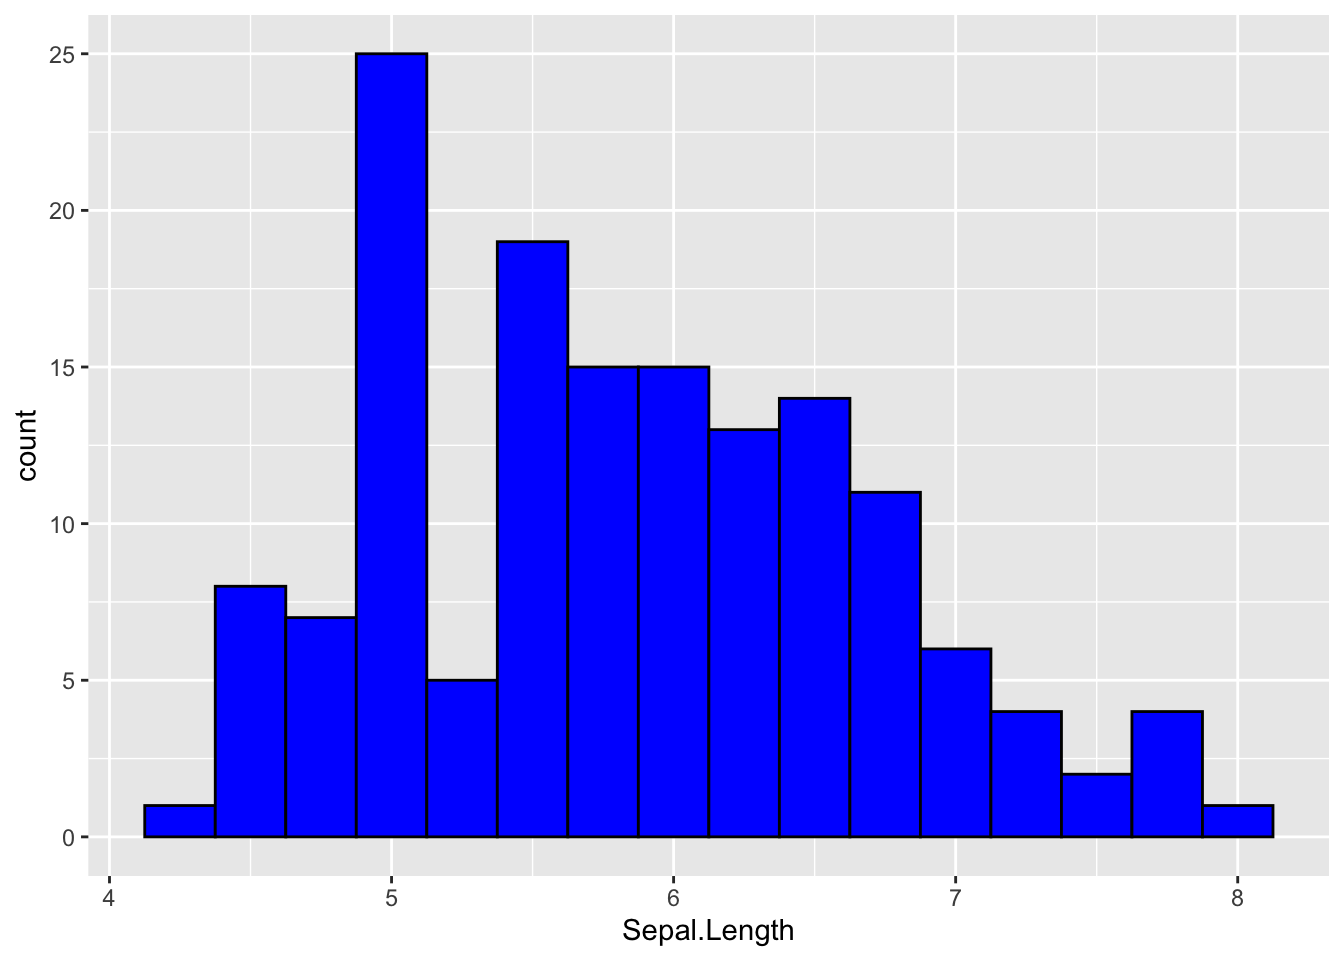
\includegraphics{_main_files/figure-latex/unnamed-chunk-40-1.pdf}

もし,このグラフのように日本語が文字化けして豆腐みたいになっていたら,フォントを指定する。

\begin{Shaded}
\begin{Highlighting}[]
\CommentTok{\#theme\_set( theme\_gray(base\_family = "IPAexGothic"))}
\FunctionTok{plot}\NormalTok{(g)}
\end{Highlighting}
\end{Shaded}

\begin{verbatim}
## Warning in grid.Call(C_textBounds, as.graphicsAnnot(x$label), x$x, x$y, :
## 'mbcsToSbcs' 中の '頻度' で変換に失敗: <e9> をドットで置き換えました
\end{verbatim}

\begin{verbatim}
## Warning in grid.Call(C_textBounds, as.graphicsAnnot(x$label), x$x, x$y, :
## 'mbcsToSbcs' 中の '頻度' で変換に失敗: <a0> をドットで置き換えました
\end{verbatim}

\begin{verbatim}
## Warning in grid.Call(C_textBounds, as.graphicsAnnot(x$label), x$x, x$y, :
## 'mbcsToSbcs' 中の '頻度' で変換に失敗: <bb> をドットで置き換えました
\end{verbatim}

\begin{verbatim}
## Warning in grid.Call(C_textBounds, as.graphicsAnnot(x$label), x$x, x$y, :
## 'mbcsToSbcs' 中の '頻度' で変換に失敗: <e5> をドットで置き換えました
\end{verbatim}

\begin{verbatim}
## Warning in grid.Call(C_textBounds, as.graphicsAnnot(x$label), x$x, x$y, :
## 'mbcsToSbcs' 中の '頻度' で変換に失敗: <ba> をドットで置き換えました
\end{verbatim}

\begin{verbatim}
## Warning in grid.Call(C_textBounds, as.graphicsAnnot(x$label), x$x, x$y, :
## 'mbcsToSbcs' 中の '頻度' で変換に失敗: <a6> をドットで置き換えました
\end{verbatim}

\begin{verbatim}
## Warning in grid.Call(C_textBounds, as.graphicsAnnot(x$label), x$x, x$y, :
## 'mbcsToSbcs' 中の '頻度' で変換に失敗: <e9> をドットで置き換えました
\end{verbatim}

\begin{verbatim}
## Warning in grid.Call(C_textBounds, as.graphicsAnnot(x$label), x$x, x$y, :
## 'mbcsToSbcs' 中の '頻度' で変換に失敗: <a0> をドットで置き換えました
\end{verbatim}

\begin{verbatim}
## Warning in grid.Call(C_textBounds, as.graphicsAnnot(x$label), x$x, x$y, :
## 'mbcsToSbcs' 中の '頻度' で変換に失敗: <bb> をドットで置き換えました
\end{verbatim}

\begin{verbatim}
## Warning in grid.Call(C_textBounds, as.graphicsAnnot(x$label), x$x, x$y, :
## 'mbcsToSbcs' 中の '頻度' で変換に失敗: <e5> をドットで置き換えました
\end{verbatim}

\begin{verbatim}
## Warning in grid.Call(C_textBounds, as.graphicsAnnot(x$label), x$x, x$y, :
## 'mbcsToSbcs' 中の '頻度' で変換に失敗: <ba> をドットで置き換えました
\end{verbatim}

\begin{verbatim}
## Warning in grid.Call(C_textBounds, as.graphicsAnnot(x$label), x$x, x$y, :
## 'mbcsToSbcs' 中の '頻度' で変換に失敗: <a6> をドットで置き換えました
\end{verbatim}

\begin{verbatim}
## Warning in grid.Call(C_textBounds, as.graphicsAnnot(x$label), x$x, x$y, :
## 'mbcsToSbcs' 中の 'アヤメの萼片長の分布' で変換に失敗: <e3> をドットで置き換えま
## した
\end{verbatim}

\begin{verbatim}
## Warning in grid.Call(C_textBounds, as.graphicsAnnot(x$label), x$x, x$y, :
## 'mbcsToSbcs' 中の 'アヤメの萼片長の分布' で変換に失敗: <82> をドットで置き換えま
## した
\end{verbatim}

\begin{verbatim}
## Warning in grid.Call(C_textBounds, as.graphicsAnnot(x$label), x$x, x$y, :
## 'mbcsToSbcs' 中の 'アヤメの萼片長の分布' で変換に失敗: <a2> をドットで置き換えま
## した
\end{verbatim}

\begin{verbatim}
## Warning in grid.Call(C_textBounds, as.graphicsAnnot(x$label), x$x, x$y, :
## 'mbcsToSbcs' 中の 'アヤメの萼片長の分布' で変換に失敗: <e3> をドットで置き換えま
## した
\end{verbatim}

\begin{verbatim}
## Warning in grid.Call(C_textBounds, as.graphicsAnnot(x$label), x$x, x$y, :
## 'mbcsToSbcs' 中の 'アヤメの萼片長の分布' で変換に失敗: <83> をドットで置き換えま
## した
\end{verbatim}

\begin{verbatim}
## Warning in grid.Call(C_textBounds, as.graphicsAnnot(x$label), x$x, x$y, :
## 'mbcsToSbcs' 中の 'アヤメの萼片長の分布' で変換に失敗: <a4> をドットで置き換えま
## した
\end{verbatim}

\begin{verbatim}
## Warning in grid.Call(C_textBounds, as.graphicsAnnot(x$label), x$x, x$y, :
## 'mbcsToSbcs' 中の 'アヤメの萼片長の分布' で変換に失敗: <e3> をドットで置き換えま
## した
\end{verbatim}

\begin{verbatim}
## Warning in grid.Call(C_textBounds, as.graphicsAnnot(x$label), x$x, x$y, :
## 'mbcsToSbcs' 中の 'アヤメの萼片長の分布' で変換に失敗: <83> をドットで置き換えま
## した
\end{verbatim}

\begin{verbatim}
## Warning in grid.Call(C_textBounds, as.graphicsAnnot(x$label), x$x, x$y, :
## 'mbcsToSbcs' 中の 'アヤメの萼片長の分布' で変換に失敗: <a1> をドットで置き換えま
## した
\end{verbatim}

\begin{verbatim}
## Warning in grid.Call(C_textBounds, as.graphicsAnnot(x$label), x$x, x$y, :
## 'mbcsToSbcs' 中の 'アヤメの萼片長の分布' で変換に失敗: <e3> をドットで置き換えま
## した
\end{verbatim}

\begin{verbatim}
## Warning in grid.Call(C_textBounds, as.graphicsAnnot(x$label), x$x, x$y, :
## 'mbcsToSbcs' 中の 'アヤメの萼片長の分布' で変換に失敗: <81> をドットで置き換えま
## した
\end{verbatim}

\begin{verbatim}
## Warning in grid.Call(C_textBounds, as.graphicsAnnot(x$label), x$x, x$y, :
## 'mbcsToSbcs' 中の 'アヤメの萼片長の分布' で変換に失敗: <ae> をドットで置き換えま
## した
\end{verbatim}

\begin{verbatim}
## Warning in grid.Call(C_textBounds, as.graphicsAnnot(x$label), x$x, x$y, :
## 'mbcsToSbcs' 中の 'アヤメの萼片長の分布' で変換に失敗: <e8> をドットで置き換えま
## した
\end{verbatim}

\begin{verbatim}
## Warning in grid.Call(C_textBounds, as.graphicsAnnot(x$label), x$x, x$y, :
## 'mbcsToSbcs' 中の 'アヤメの萼片長の分布' で変換に失敗: <90> をドットで置き換えま
## した
\end{verbatim}

\begin{verbatim}
## Warning in grid.Call(C_textBounds, as.graphicsAnnot(x$label), x$x, x$y, :
## 'mbcsToSbcs' 中の 'アヤメの萼片長の分布' で変換に失敗: <bc> をドットで置き換えま
## した
\end{verbatim}

\begin{verbatim}
## Warning in grid.Call(C_textBounds, as.graphicsAnnot(x$label), x$x, x$y, :
## 'mbcsToSbcs' 中の 'アヤメの萼片長の分布' で変換に失敗: <e7> をドットで置き換えま
## した
\end{verbatim}

\begin{verbatim}
## Warning in grid.Call(C_textBounds, as.graphicsAnnot(x$label), x$x, x$y, :
## 'mbcsToSbcs' 中の 'アヤメの萼片長の分布' で変換に失敗: <89> をドットで置き換えま
## した
\end{verbatim}

\begin{verbatim}
## Warning in grid.Call(C_textBounds, as.graphicsAnnot(x$label), x$x, x$y, :
## 'mbcsToSbcs' 中の 'アヤメの萼片長の分布' で変換に失敗: <87> をドットで置き換えま
## した
\end{verbatim}

\begin{verbatim}
## Warning in grid.Call(C_textBounds, as.graphicsAnnot(x$label), x$x, x$y, :
## 'mbcsToSbcs' 中の 'アヤメの萼片長の分布' で変換に失敗: <e9> をドットで置き換えま
## した
\end{verbatim}

\begin{verbatim}
## Warning in grid.Call(C_textBounds, as.graphicsAnnot(x$label), x$x, x$y, :
## 'mbcsToSbcs' 中の 'アヤメの萼片長の分布' で変換に失敗: <95> をドットで置き換えま
## した
\end{verbatim}

\begin{verbatim}
## Warning in grid.Call(C_textBounds, as.graphicsAnnot(x$label), x$x, x$y, :
## 'mbcsToSbcs' 中の 'アヤメの萼片長の分布' で変換に失敗: <b7> をドットで置き換えま
## した
\end{verbatim}

\begin{verbatim}
## Warning in grid.Call(C_textBounds, as.graphicsAnnot(x$label), x$x, x$y, :
## 'mbcsToSbcs' 中の 'アヤメの萼片長の分布' で変換に失敗: <e3> をドットで置き換えま
## した
\end{verbatim}

\begin{verbatim}
## Warning in grid.Call(C_textBounds, as.graphicsAnnot(x$label), x$x, x$y, :
## 'mbcsToSbcs' 中の 'アヤメの萼片長の分布' で変換に失敗: <81> をドットで置き換えま
## した
\end{verbatim}

\begin{verbatim}
## Warning in grid.Call(C_textBounds, as.graphicsAnnot(x$label), x$x, x$y, :
## 'mbcsToSbcs' 中の 'アヤメの萼片長の分布' で変換に失敗: <ae> をドットで置き換えま
## した
\end{verbatim}

\begin{verbatim}
## Warning in grid.Call(C_textBounds, as.graphicsAnnot(x$label), x$x, x$y, :
## 'mbcsToSbcs' 中の 'アヤメの萼片長の分布' で変換に失敗: <e5> をドットで置き換えま
## した
\end{verbatim}

\begin{verbatim}
## Warning in grid.Call(C_textBounds, as.graphicsAnnot(x$label), x$x, x$y, :
## 'mbcsToSbcs' 中の 'アヤメの萼片長の分布' で変換に失敗: <88> をドットで置き換えま
## した
\end{verbatim}

\begin{verbatim}
## Warning in grid.Call(C_textBounds, as.graphicsAnnot(x$label), x$x, x$y, :
## 'mbcsToSbcs' 中の 'アヤメの萼片長の分布' で変換に失敗: <86> をドットで置き換えま
## した
\end{verbatim}

\begin{verbatim}
## Warning in grid.Call(C_textBounds, as.graphicsAnnot(x$label), x$x, x$y, :
## 'mbcsToSbcs' 中の 'アヤメの萼片長の分布' で変換に失敗: <e5> をドットで置き換えま
## した
\end{verbatim}

\begin{verbatim}
## Warning in grid.Call(C_textBounds, as.graphicsAnnot(x$label), x$x, x$y, :
## 'mbcsToSbcs' 中の 'アヤメの萼片長の分布' で変換に失敗: <b8> をドットで置き換えま
## した
\end{verbatim}

\begin{verbatim}
## Warning in grid.Call(C_textBounds, as.graphicsAnnot(x$label), x$x, x$y, :
## 'mbcsToSbcs' 中の 'アヤメの萼片長の分布' で変換に失敗: <83> をドットで置き換えま
## した
\end{verbatim}

\begin{verbatim}
## Warning in grid.Call(C_textBounds, as.graphicsAnnot(x$label), x$x, x$y, :
## 'mbcsToSbcs' 中の 'アヤメの萼片長の分布' で変換に失敗: <e3> をドットで置き換えま
## した
\end{verbatim}

\begin{verbatim}
## Warning in grid.Call(C_textBounds, as.graphicsAnnot(x$label), x$x, x$y, :
## 'mbcsToSbcs' 中の 'アヤメの萼片長の分布' で変換に失敗: <82> をドットで置き換えま
## した
\end{verbatim}

\begin{verbatim}
## Warning in grid.Call(C_textBounds, as.graphicsAnnot(x$label), x$x, x$y, :
## 'mbcsToSbcs' 中の 'アヤメの萼片長の分布' で変換に失敗: <a2> をドットで置き換えま
## した
\end{verbatim}

\begin{verbatim}
## Warning in grid.Call(C_textBounds, as.graphicsAnnot(x$label), x$x, x$y, :
## 'mbcsToSbcs' 中の 'アヤメの萼片長の分布' で変換に失敗: <e3> をドットで置き換えま
## した
\end{verbatim}

\begin{verbatim}
## Warning in grid.Call(C_textBounds, as.graphicsAnnot(x$label), x$x, x$y, :
## 'mbcsToSbcs' 中の 'アヤメの萼片長の分布' で変換に失敗: <83> をドットで置き換えま
## した
\end{verbatim}

\begin{verbatim}
## Warning in grid.Call(C_textBounds, as.graphicsAnnot(x$label), x$x, x$y, :
## 'mbcsToSbcs' 中の 'アヤメの萼片長の分布' で変換に失敗: <a4> をドットで置き換えま
## した
\end{verbatim}

\begin{verbatim}
## Warning in grid.Call(C_textBounds, as.graphicsAnnot(x$label), x$x, x$y, :
## 'mbcsToSbcs' 中の 'アヤメの萼片長の分布' で変換に失敗: <e3> をドットで置き換えま
## した
\end{verbatim}

\begin{verbatim}
## Warning in grid.Call(C_textBounds, as.graphicsAnnot(x$label), x$x, x$y, :
## 'mbcsToSbcs' 中の 'アヤメの萼片長の分布' で変換に失敗: <83> をドットで置き換えま
## した
\end{verbatim}

\begin{verbatim}
## Warning in grid.Call(C_textBounds, as.graphicsAnnot(x$label), x$x, x$y, :
## 'mbcsToSbcs' 中の 'アヤメの萼片長の分布' で変換に失敗: <a1> をドットで置き換えま
## した
\end{verbatim}

\begin{verbatim}
## Warning in grid.Call(C_textBounds, as.graphicsAnnot(x$label), x$x, x$y, :
## 'mbcsToSbcs' 中の 'アヤメの萼片長の分布' で変換に失敗: <e3> をドットで置き換えま
## した
\end{verbatim}

\begin{verbatim}
## Warning in grid.Call(C_textBounds, as.graphicsAnnot(x$label), x$x, x$y, :
## 'mbcsToSbcs' 中の 'アヤメの萼片長の分布' で変換に失敗: <81> をドットで置き換えま
## した
\end{verbatim}

\begin{verbatim}
## Warning in grid.Call(C_textBounds, as.graphicsAnnot(x$label), x$x, x$y, :
## 'mbcsToSbcs' 中の 'アヤメの萼片長の分布' で変換に失敗: <ae> をドットで置き換えま
## した
\end{verbatim}

\begin{verbatim}
## Warning in grid.Call(C_textBounds, as.graphicsAnnot(x$label), x$x, x$y, :
## 'mbcsToSbcs' 中の 'アヤメの萼片長の分布' で変換に失敗: <e8> をドットで置き換えま
## した
\end{verbatim}

\begin{verbatim}
## Warning in grid.Call(C_textBounds, as.graphicsAnnot(x$label), x$x, x$y, :
## 'mbcsToSbcs' 中の 'アヤメの萼片長の分布' で変換に失敗: <90> をドットで置き換えま
## した
\end{verbatim}

\begin{verbatim}
## Warning in grid.Call(C_textBounds, as.graphicsAnnot(x$label), x$x, x$y, :
## 'mbcsToSbcs' 中の 'アヤメの萼片長の分布' で変換に失敗: <bc> をドットで置き換えま
## した
\end{verbatim}

\begin{verbatim}
## Warning in grid.Call(C_textBounds, as.graphicsAnnot(x$label), x$x, x$y, :
## 'mbcsToSbcs' 中の 'アヤメの萼片長の分布' で変換に失敗: <e7> をドットで置き換えま
## した
\end{verbatim}

\begin{verbatim}
## Warning in grid.Call(C_textBounds, as.graphicsAnnot(x$label), x$x, x$y, :
## 'mbcsToSbcs' 中の 'アヤメの萼片長の分布' で変換に失敗: <89> をドットで置き換えま
## した
\end{verbatim}

\begin{verbatim}
## Warning in grid.Call(C_textBounds, as.graphicsAnnot(x$label), x$x, x$y, :
## 'mbcsToSbcs' 中の 'アヤメの萼片長の分布' で変換に失敗: <87> をドットで置き換えま
## した
\end{verbatim}

\begin{verbatim}
## Warning in grid.Call(C_textBounds, as.graphicsAnnot(x$label), x$x, x$y, :
## 'mbcsToSbcs' 中の 'アヤメの萼片長の分布' で変換に失敗: <e9> をドットで置き換えま
## した
\end{verbatim}

\begin{verbatim}
## Warning in grid.Call(C_textBounds, as.graphicsAnnot(x$label), x$x, x$y, :
## 'mbcsToSbcs' 中の 'アヤメの萼片長の分布' で変換に失敗: <95> をドットで置き換えま
## した
\end{verbatim}

\begin{verbatim}
## Warning in grid.Call(C_textBounds, as.graphicsAnnot(x$label), x$x, x$y, :
## 'mbcsToSbcs' 中の 'アヤメの萼片長の分布' で変換に失敗: <b7> をドットで置き換えま
## した
\end{verbatim}

\begin{verbatim}
## Warning in grid.Call(C_textBounds, as.graphicsAnnot(x$label), x$x, x$y, :
## 'mbcsToSbcs' 中の 'アヤメの萼片長の分布' で変換に失敗: <e3> をドットで置き換えま
## した
\end{verbatim}

\begin{verbatim}
## Warning in grid.Call(C_textBounds, as.graphicsAnnot(x$label), x$x, x$y, :
## 'mbcsToSbcs' 中の 'アヤメの萼片長の分布' で変換に失敗: <81> をドットで置き換えま
## した
\end{verbatim}

\begin{verbatim}
## Warning in grid.Call(C_textBounds, as.graphicsAnnot(x$label), x$x, x$y, :
## 'mbcsToSbcs' 中の 'アヤメの萼片長の分布' で変換に失敗: <ae> をドットで置き換えま
## した
\end{verbatim}

\begin{verbatim}
## Warning in grid.Call(C_textBounds, as.graphicsAnnot(x$label), x$x, x$y, :
## 'mbcsToSbcs' 中の 'アヤメの萼片長の分布' で変換に失敗: <e5> をドットで置き換えま
## した
\end{verbatim}

\begin{verbatim}
## Warning in grid.Call(C_textBounds, as.graphicsAnnot(x$label), x$x, x$y, :
## 'mbcsToSbcs' 中の 'アヤメの萼片長の分布' で変換に失敗: <88> をドットで置き換えま
## した
\end{verbatim}

\begin{verbatim}
## Warning in grid.Call(C_textBounds, as.graphicsAnnot(x$label), x$x, x$y, :
## 'mbcsToSbcs' 中の 'アヤメの萼片長の分布' で変換に失敗: <86> をドットで置き換えま
## した
\end{verbatim}

\begin{verbatim}
## Warning in grid.Call(C_textBounds, as.graphicsAnnot(x$label), x$x, x$y, :
## 'mbcsToSbcs' 中の 'アヤメの萼片長の分布' で変換に失敗: <e5> をドットで置き換えま
## した
\end{verbatim}

\begin{verbatim}
## Warning in grid.Call(C_textBounds, as.graphicsAnnot(x$label), x$x, x$y, :
## 'mbcsToSbcs' 中の 'アヤメの萼片長の分布' で変換に失敗: <b8> をドットで置き換えま
## した
\end{verbatim}

\begin{verbatim}
## Warning in grid.Call(C_textBounds, as.graphicsAnnot(x$label), x$x, x$y, :
## 'mbcsToSbcs' 中の 'アヤメの萼片長の分布' で変換に失敗: <83> をドットで置き換えま
## した
\end{verbatim}

\begin{verbatim}
## Warning in grid.Call(C_textBounds, as.graphicsAnnot(x$label), x$x, x$y, :
## 'mbcsToSbcs' 中の '萼片長' で変換に失敗: <e8> をドットで置き換えました
\end{verbatim}

\begin{verbatim}
## Warning in grid.Call(C_textBounds, as.graphicsAnnot(x$label), x$x, x$y, :
## 'mbcsToSbcs' 中の '萼片長' で変換に失敗: <90> をドットで置き換えました
\end{verbatim}

\begin{verbatim}
## Warning in grid.Call(C_textBounds, as.graphicsAnnot(x$label), x$x, x$y, :
## 'mbcsToSbcs' 中の '萼片長' で変換に失敗: <bc> をドットで置き換えました
\end{verbatim}

\begin{verbatim}
## Warning in grid.Call(C_textBounds, as.graphicsAnnot(x$label), x$x, x$y, :
## 'mbcsToSbcs' 中の '萼片長' で変換に失敗: <e7> をドットで置き換えました
\end{verbatim}

\begin{verbatim}
## Warning in grid.Call(C_textBounds, as.graphicsAnnot(x$label), x$x, x$y, :
## 'mbcsToSbcs' 中の '萼片長' で変換に失敗: <89> をドットで置き換えました
\end{verbatim}

\begin{verbatim}
## Warning in grid.Call(C_textBounds, as.graphicsAnnot(x$label), x$x, x$y, :
## 'mbcsToSbcs' 中の '萼片長' で変換に失敗: <87> をドットで置き換えました
\end{verbatim}

\begin{verbatim}
## Warning in grid.Call(C_textBounds, as.graphicsAnnot(x$label), x$x, x$y, :
## 'mbcsToSbcs' 中の '萼片長' で変換に失敗: <e9> をドットで置き換えました
\end{verbatim}

\begin{verbatim}
## Warning in grid.Call(C_textBounds, as.graphicsAnnot(x$label), x$x, x$y, :
## 'mbcsToSbcs' 中の '萼片長' で変換に失敗: <95> をドットで置き換えました
\end{verbatim}

\begin{verbatim}
## Warning in grid.Call(C_textBounds, as.graphicsAnnot(x$label), x$x, x$y, :
## 'mbcsToSbcs' 中の '萼片長' で変換に失敗: <b7> をドットで置き換えました
\end{verbatim}

\begin{verbatim}
## Warning in grid.Call(C_textBounds, as.graphicsAnnot(x$label), x$x, x$y, :
## 'mbcsToSbcs' 中の '萼片長' で変換に失敗: <e8> をドットで置き換えました
\end{verbatim}

\begin{verbatim}
## Warning in grid.Call(C_textBounds, as.graphicsAnnot(x$label), x$x, x$y, :
## 'mbcsToSbcs' 中の '萼片長' で変換に失敗: <90> をドットで置き換えました
\end{verbatim}

\begin{verbatim}
## Warning in grid.Call(C_textBounds, as.graphicsAnnot(x$label), x$x, x$y, :
## 'mbcsToSbcs' 中の '萼片長' で変換に失敗: <bc> をドットで置き換えました
\end{verbatim}

\begin{verbatim}
## Warning in grid.Call(C_textBounds, as.graphicsAnnot(x$label), x$x, x$y, :
## 'mbcsToSbcs' 中の '萼片長' で変換に失敗: <e7> をドットで置き換えました
\end{verbatim}

\begin{verbatim}
## Warning in grid.Call(C_textBounds, as.graphicsAnnot(x$label), x$x, x$y, :
## 'mbcsToSbcs' 中の '萼片長' で変換に失敗: <89> をドットで置き換えました
\end{verbatim}

\begin{verbatim}
## Warning in grid.Call(C_textBounds, as.graphicsAnnot(x$label), x$x, x$y, :
## 'mbcsToSbcs' 中の '萼片長' で変換に失敗: <87> をドットで置き換えました
\end{verbatim}

\begin{verbatim}
## Warning in grid.Call(C_textBounds, as.graphicsAnnot(x$label), x$x, x$y, :
## 'mbcsToSbcs' 中の '萼片長' で変換に失敗: <e9> をドットで置き換えました
\end{verbatim}

\begin{verbatim}
## Warning in grid.Call(C_textBounds, as.graphicsAnnot(x$label), x$x, x$y, :
## 'mbcsToSbcs' 中の '萼片長' で変換に失敗: <95> をドットで置き換えました
\end{verbatim}

\begin{verbatim}
## Warning in grid.Call(C_textBounds, as.graphicsAnnot(x$label), x$x, x$y, :
## 'mbcsToSbcs' 中の '萼片長' で変換に失敗: <b7> をドットで置き換えました
\end{verbatim}

\begin{verbatim}
## Warning in grid.Call(C_textBounds, as.graphicsAnnot(x$label), x$x, x$y, :
## 'mbcsToSbcs' 中の '頻度' で変換に失敗: <e9> をドットで置き換えました
\end{verbatim}

\begin{verbatim}
## Warning in grid.Call(C_textBounds, as.graphicsAnnot(x$label), x$x, x$y, :
## 'mbcsToSbcs' 中の '頻度' で変換に失敗: <a0> をドットで置き換えました
\end{verbatim}

\begin{verbatim}
## Warning in grid.Call(C_textBounds, as.graphicsAnnot(x$label), x$x, x$y, :
## 'mbcsToSbcs' 中の '頻度' で変換に失敗: <bb> をドットで置き換えました
\end{verbatim}

\begin{verbatim}
## Warning in grid.Call(C_textBounds, as.graphicsAnnot(x$label), x$x, x$y, :
## 'mbcsToSbcs' 中の '頻度' で変換に失敗: <e5> をドットで置き換えました
\end{verbatim}

\begin{verbatim}
## Warning in grid.Call(C_textBounds, as.graphicsAnnot(x$label), x$x, x$y, :
## 'mbcsToSbcs' 中の '頻度' で変換に失敗: <ba> をドットで置き換えました
\end{verbatim}

\begin{verbatim}
## Warning in grid.Call(C_textBounds, as.graphicsAnnot(x$label), x$x, x$y, :
## 'mbcsToSbcs' 中の '頻度' で変換に失敗: <a6> をドットで置き換えました
\end{verbatim}

\begin{verbatim}
## Warning in grid.Call(C_textBounds, as.graphicsAnnot(x$label), x$x, x$y, :
## 'mbcsToSbcs' 中の '頻度' で変換に失敗: <e9> をドットで置き換えました
\end{verbatim}

\begin{verbatim}
## Warning in grid.Call(C_textBounds, as.graphicsAnnot(x$label), x$x, x$y, :
## 'mbcsToSbcs' 中の '頻度' で変換に失敗: <a0> をドットで置き換えました
\end{verbatim}

\begin{verbatim}
## Warning in grid.Call(C_textBounds, as.graphicsAnnot(x$label), x$x, x$y, :
## 'mbcsToSbcs' 中の '頻度' で変換に失敗: <bb> をドットで置き換えました
\end{verbatim}

\begin{verbatim}
## Warning in grid.Call(C_textBounds, as.graphicsAnnot(x$label), x$x, x$y, :
## 'mbcsToSbcs' 中の '頻度' で変換に失敗: <e5> をドットで置き換えました
\end{verbatim}

\begin{verbatim}
## Warning in grid.Call(C_textBounds, as.graphicsAnnot(x$label), x$x, x$y, :
## 'mbcsToSbcs' 中の '頻度' で変換に失敗: <ba> をドットで置き換えました
\end{verbatim}

\begin{verbatim}
## Warning in grid.Call(C_textBounds, as.graphicsAnnot(x$label), x$x, x$y, :
## 'mbcsToSbcs' 中の '頻度' で変換に失敗: <a6> をドットで置き換えました
\end{verbatim}

\begin{verbatim}
## Warning in grid.Call(C_textBounds, as.graphicsAnnot(x$label), x$x, x$y, :
## 'mbcsToSbcs' 中の '頻度' で変換に失敗: <e9> をドットで置き換えました
\end{verbatim}

\begin{verbatim}
## Warning in grid.Call(C_textBounds, as.graphicsAnnot(x$label), x$x, x$y, :
## 'mbcsToSbcs' 中の '頻度' で変換に失敗: <a0> をドットで置き換えました
\end{verbatim}

\begin{verbatim}
## Warning in grid.Call(C_textBounds, as.graphicsAnnot(x$label), x$x, x$y, :
## 'mbcsToSbcs' 中の '頻度' で変換に失敗: <bb> をドットで置き換えました
\end{verbatim}

\begin{verbatim}
## Warning in grid.Call(C_textBounds, as.graphicsAnnot(x$label), x$x, x$y, :
## 'mbcsToSbcs' 中の '頻度' で変換に失敗: <e5> をドットで置き換えました
\end{verbatim}

\begin{verbatim}
## Warning in grid.Call(C_textBounds, as.graphicsAnnot(x$label), x$x, x$y, :
## 'mbcsToSbcs' 中の '頻度' で変換に失敗: <ba> をドットで置き換えました
\end{verbatim}

\begin{verbatim}
## Warning in grid.Call(C_textBounds, as.graphicsAnnot(x$label), x$x, x$y, :
## 'mbcsToSbcs' 中の '頻度' で変換に失敗: <a6> をドットで置き換えました
\end{verbatim}

\begin{verbatim}
## Warning in grid.Call(C_textBounds, as.graphicsAnnot(x$label), x$x, x$y, :
## 'mbcsToSbcs' 中の 'アヤメの萼片長の分布' で変換に失敗: <e3> をドットで置き換えま
## した
\end{verbatim}

\begin{verbatim}
## Warning in grid.Call(C_textBounds, as.graphicsAnnot(x$label), x$x, x$y, :
## 'mbcsToSbcs' 中の 'アヤメの萼片長の分布' で変換に失敗: <82> をドットで置き換えま
## した
\end{verbatim}

\begin{verbatim}
## Warning in grid.Call(C_textBounds, as.graphicsAnnot(x$label), x$x, x$y, :
## 'mbcsToSbcs' 中の 'アヤメの萼片長の分布' で変換に失敗: <a2> をドットで置き換えま
## した
\end{verbatim}

\begin{verbatim}
## Warning in grid.Call(C_textBounds, as.graphicsAnnot(x$label), x$x, x$y, :
## 'mbcsToSbcs' 中の 'アヤメの萼片長の分布' で変換に失敗: <e3> をドットで置き換えま
## した
\end{verbatim}

\begin{verbatim}
## Warning in grid.Call(C_textBounds, as.graphicsAnnot(x$label), x$x, x$y, :
## 'mbcsToSbcs' 中の 'アヤメの萼片長の分布' で変換に失敗: <83> をドットで置き換えま
## した
\end{verbatim}

\begin{verbatim}
## Warning in grid.Call(C_textBounds, as.graphicsAnnot(x$label), x$x, x$y, :
## 'mbcsToSbcs' 中の 'アヤメの萼片長の分布' で変換に失敗: <a4> をドットで置き換えま
## した
\end{verbatim}

\begin{verbatim}
## Warning in grid.Call(C_textBounds, as.graphicsAnnot(x$label), x$x, x$y, :
## 'mbcsToSbcs' 中の 'アヤメの萼片長の分布' で変換に失敗: <e3> をドットで置き換えま
## した
\end{verbatim}

\begin{verbatim}
## Warning in grid.Call(C_textBounds, as.graphicsAnnot(x$label), x$x, x$y, :
## 'mbcsToSbcs' 中の 'アヤメの萼片長の分布' で変換に失敗: <83> をドットで置き換えま
## した
\end{verbatim}

\begin{verbatim}
## Warning in grid.Call(C_textBounds, as.graphicsAnnot(x$label), x$x, x$y, :
## 'mbcsToSbcs' 中の 'アヤメの萼片長の分布' で変換に失敗: <a1> をドットで置き換えま
## した
\end{verbatim}

\begin{verbatim}
## Warning in grid.Call(C_textBounds, as.graphicsAnnot(x$label), x$x, x$y, :
## 'mbcsToSbcs' 中の 'アヤメの萼片長の分布' で変換に失敗: <e3> をドットで置き換えま
## した
\end{verbatim}

\begin{verbatim}
## Warning in grid.Call(C_textBounds, as.graphicsAnnot(x$label), x$x, x$y, :
## 'mbcsToSbcs' 中の 'アヤメの萼片長の分布' で変換に失敗: <81> をドットで置き換えま
## した
\end{verbatim}

\begin{verbatim}
## Warning in grid.Call(C_textBounds, as.graphicsAnnot(x$label), x$x, x$y, :
## 'mbcsToSbcs' 中の 'アヤメの萼片長の分布' で変換に失敗: <ae> をドットで置き換えま
## した
\end{verbatim}

\begin{verbatim}
## Warning in grid.Call(C_textBounds, as.graphicsAnnot(x$label), x$x, x$y, :
## 'mbcsToSbcs' 中の 'アヤメの萼片長の分布' で変換に失敗: <e8> をドットで置き換えま
## した
\end{verbatim}

\begin{verbatim}
## Warning in grid.Call(C_textBounds, as.graphicsAnnot(x$label), x$x, x$y, :
## 'mbcsToSbcs' 中の 'アヤメの萼片長の分布' で変換に失敗: <90> をドットで置き換えま
## した
\end{verbatim}

\begin{verbatim}
## Warning in grid.Call(C_textBounds, as.graphicsAnnot(x$label), x$x, x$y, :
## 'mbcsToSbcs' 中の 'アヤメの萼片長の分布' で変換に失敗: <bc> をドットで置き換えま
## した
\end{verbatim}

\begin{verbatim}
## Warning in grid.Call(C_textBounds, as.graphicsAnnot(x$label), x$x, x$y, :
## 'mbcsToSbcs' 中の 'アヤメの萼片長の分布' で変換に失敗: <e7> をドットで置き換えま
## した
\end{verbatim}

\begin{verbatim}
## Warning in grid.Call(C_textBounds, as.graphicsAnnot(x$label), x$x, x$y, :
## 'mbcsToSbcs' 中の 'アヤメの萼片長の分布' で変換に失敗: <89> をドットで置き換えま
## した
\end{verbatim}

\begin{verbatim}
## Warning in grid.Call(C_textBounds, as.graphicsAnnot(x$label), x$x, x$y, :
## 'mbcsToSbcs' 中の 'アヤメの萼片長の分布' で変換に失敗: <87> をドットで置き換えま
## した
\end{verbatim}

\begin{verbatim}
## Warning in grid.Call(C_textBounds, as.graphicsAnnot(x$label), x$x, x$y, :
## 'mbcsToSbcs' 中の 'アヤメの萼片長の分布' で変換に失敗: <e9> をドットで置き換えま
## した
\end{verbatim}

\begin{verbatim}
## Warning in grid.Call(C_textBounds, as.graphicsAnnot(x$label), x$x, x$y, :
## 'mbcsToSbcs' 中の 'アヤメの萼片長の分布' で変換に失敗: <95> をドットで置き換えま
## した
\end{verbatim}

\begin{verbatim}
## Warning in grid.Call(C_textBounds, as.graphicsAnnot(x$label), x$x, x$y, :
## 'mbcsToSbcs' 中の 'アヤメの萼片長の分布' で変換に失敗: <b7> をドットで置き換えま
## した
\end{verbatim}

\begin{verbatim}
## Warning in grid.Call(C_textBounds, as.graphicsAnnot(x$label), x$x, x$y, :
## 'mbcsToSbcs' 中の 'アヤメの萼片長の分布' で変換に失敗: <e3> をドットで置き換えま
## した
\end{verbatim}

\begin{verbatim}
## Warning in grid.Call(C_textBounds, as.graphicsAnnot(x$label), x$x, x$y, :
## 'mbcsToSbcs' 中の 'アヤメの萼片長の分布' で変換に失敗: <81> をドットで置き換えま
## した
\end{verbatim}

\begin{verbatim}
## Warning in grid.Call(C_textBounds, as.graphicsAnnot(x$label), x$x, x$y, :
## 'mbcsToSbcs' 中の 'アヤメの萼片長の分布' で変換に失敗: <ae> をドットで置き換えま
## した
\end{verbatim}

\begin{verbatim}
## Warning in grid.Call(C_textBounds, as.graphicsAnnot(x$label), x$x, x$y, :
## 'mbcsToSbcs' 中の 'アヤメの萼片長の分布' で変換に失敗: <e5> をドットで置き換えま
## した
\end{verbatim}

\begin{verbatim}
## Warning in grid.Call(C_textBounds, as.graphicsAnnot(x$label), x$x, x$y, :
## 'mbcsToSbcs' 中の 'アヤメの萼片長の分布' で変換に失敗: <88> をドットで置き換えま
## した
\end{verbatim}

\begin{verbatim}
## Warning in grid.Call(C_textBounds, as.graphicsAnnot(x$label), x$x, x$y, :
## 'mbcsToSbcs' 中の 'アヤメの萼片長の分布' で変換に失敗: <86> をドットで置き換えま
## した
\end{verbatim}

\begin{verbatim}
## Warning in grid.Call(C_textBounds, as.graphicsAnnot(x$label), x$x, x$y, :
## 'mbcsToSbcs' 中の 'アヤメの萼片長の分布' で変換に失敗: <e5> をドットで置き換えま
## した
\end{verbatim}

\begin{verbatim}
## Warning in grid.Call(C_textBounds, as.graphicsAnnot(x$label), x$x, x$y, :
## 'mbcsToSbcs' 中の 'アヤメの萼片長の分布' で変換に失敗: <b8> をドットで置き換えま
## した
\end{verbatim}

\begin{verbatim}
## Warning in grid.Call(C_textBounds, as.graphicsAnnot(x$label), x$x, x$y, :
## 'mbcsToSbcs' 中の 'アヤメの萼片長の分布' で変換に失敗: <83> をドットで置き換えま
## した
\end{verbatim}

\begin{verbatim}
## Warning in grid.Call(C_textBounds, as.graphicsAnnot(x$label), x$x, x$y, :
## 'mbcsToSbcs' 中の 'アヤメの萼片長の分布' で変換に失敗: <e3> をドットで置き換えま
## した
\end{verbatim}

\begin{verbatim}
## Warning in grid.Call(C_textBounds, as.graphicsAnnot(x$label), x$x, x$y, :
## 'mbcsToSbcs' 中の 'アヤメの萼片長の分布' で変換に失敗: <82> をドットで置き換えま
## した
\end{verbatim}

\begin{verbatim}
## Warning in grid.Call(C_textBounds, as.graphicsAnnot(x$label), x$x, x$y, :
## 'mbcsToSbcs' 中の 'アヤメの萼片長の分布' で変換に失敗: <a2> をドットで置き換えま
## した
\end{verbatim}

\begin{verbatim}
## Warning in grid.Call(C_textBounds, as.graphicsAnnot(x$label), x$x, x$y, :
## 'mbcsToSbcs' 中の 'アヤメの萼片長の分布' で変換に失敗: <e3> をドットで置き換えま
## した
\end{verbatim}

\begin{verbatim}
## Warning in grid.Call(C_textBounds, as.graphicsAnnot(x$label), x$x, x$y, :
## 'mbcsToSbcs' 中の 'アヤメの萼片長の分布' で変換に失敗: <83> をドットで置き換えま
## した
\end{verbatim}

\begin{verbatim}
## Warning in grid.Call(C_textBounds, as.graphicsAnnot(x$label), x$x, x$y, :
## 'mbcsToSbcs' 中の 'アヤメの萼片長の分布' で変換に失敗: <a4> をドットで置き換えま
## した
\end{verbatim}

\begin{verbatim}
## Warning in grid.Call(C_textBounds, as.graphicsAnnot(x$label), x$x, x$y, :
## 'mbcsToSbcs' 中の 'アヤメの萼片長の分布' で変換に失敗: <e3> をドットで置き換えま
## した
\end{verbatim}

\begin{verbatim}
## Warning in grid.Call(C_textBounds, as.graphicsAnnot(x$label), x$x, x$y, :
## 'mbcsToSbcs' 中の 'アヤメの萼片長の分布' で変換に失敗: <83> をドットで置き換えま
## した
\end{verbatim}

\begin{verbatim}
## Warning in grid.Call(C_textBounds, as.graphicsAnnot(x$label), x$x, x$y, :
## 'mbcsToSbcs' 中の 'アヤメの萼片長の分布' で変換に失敗: <a1> をドットで置き換えま
## した
\end{verbatim}

\begin{verbatim}
## Warning in grid.Call(C_textBounds, as.graphicsAnnot(x$label), x$x, x$y, :
## 'mbcsToSbcs' 中の 'アヤメの萼片長の分布' で変換に失敗: <e3> をドットで置き換えま
## した
\end{verbatim}

\begin{verbatim}
## Warning in grid.Call(C_textBounds, as.graphicsAnnot(x$label), x$x, x$y, :
## 'mbcsToSbcs' 中の 'アヤメの萼片長の分布' で変換に失敗: <81> をドットで置き換えま
## した
\end{verbatim}

\begin{verbatim}
## Warning in grid.Call(C_textBounds, as.graphicsAnnot(x$label), x$x, x$y, :
## 'mbcsToSbcs' 中の 'アヤメの萼片長の分布' で変換に失敗: <ae> をドットで置き換えま
## した
\end{verbatim}

\begin{verbatim}
## Warning in grid.Call(C_textBounds, as.graphicsAnnot(x$label), x$x, x$y, :
## 'mbcsToSbcs' 中の 'アヤメの萼片長の分布' で変換に失敗: <e8> をドットで置き換えま
## した
\end{verbatim}

\begin{verbatim}
## Warning in grid.Call(C_textBounds, as.graphicsAnnot(x$label), x$x, x$y, :
## 'mbcsToSbcs' 中の 'アヤメの萼片長の分布' で変換に失敗: <90> をドットで置き換えま
## した
\end{verbatim}

\begin{verbatim}
## Warning in grid.Call(C_textBounds, as.graphicsAnnot(x$label), x$x, x$y, :
## 'mbcsToSbcs' 中の 'アヤメの萼片長の分布' で変換に失敗: <bc> をドットで置き換えま
## した
\end{verbatim}

\begin{verbatim}
## Warning in grid.Call(C_textBounds, as.graphicsAnnot(x$label), x$x, x$y, :
## 'mbcsToSbcs' 中の 'アヤメの萼片長の分布' で変換に失敗: <e7> をドットで置き換えま
## した
\end{verbatim}

\begin{verbatim}
## Warning in grid.Call(C_textBounds, as.graphicsAnnot(x$label), x$x, x$y, :
## 'mbcsToSbcs' 中の 'アヤメの萼片長の分布' で変換に失敗: <89> をドットで置き換えま
## した
\end{verbatim}

\begin{verbatim}
## Warning in grid.Call(C_textBounds, as.graphicsAnnot(x$label), x$x, x$y, :
## 'mbcsToSbcs' 中の 'アヤメの萼片長の分布' で変換に失敗: <87> をドットで置き換えま
## した
\end{verbatim}

\begin{verbatim}
## Warning in grid.Call(C_textBounds, as.graphicsAnnot(x$label), x$x, x$y, :
## 'mbcsToSbcs' 中の 'アヤメの萼片長の分布' で変換に失敗: <e9> をドットで置き換えま
## した
\end{verbatim}

\begin{verbatim}
## Warning in grid.Call(C_textBounds, as.graphicsAnnot(x$label), x$x, x$y, :
## 'mbcsToSbcs' 中の 'アヤメの萼片長の分布' で変換に失敗: <95> をドットで置き換えま
## した
\end{verbatim}

\begin{verbatim}
## Warning in grid.Call(C_textBounds, as.graphicsAnnot(x$label), x$x, x$y, :
## 'mbcsToSbcs' 中の 'アヤメの萼片長の分布' で変換に失敗: <b7> をドットで置き換えま
## した
\end{verbatim}

\begin{verbatim}
## Warning in grid.Call(C_textBounds, as.graphicsAnnot(x$label), x$x, x$y, :
## 'mbcsToSbcs' 中の 'アヤメの萼片長の分布' で変換に失敗: <e3> をドットで置き換えま
## した
\end{verbatim}

\begin{verbatim}
## Warning in grid.Call(C_textBounds, as.graphicsAnnot(x$label), x$x, x$y, :
## 'mbcsToSbcs' 中の 'アヤメの萼片長の分布' で変換に失敗: <81> をドットで置き換えま
## した
\end{verbatim}

\begin{verbatim}
## Warning in grid.Call(C_textBounds, as.graphicsAnnot(x$label), x$x, x$y, :
## 'mbcsToSbcs' 中の 'アヤメの萼片長の分布' で変換に失敗: <ae> をドットで置き換えま
## した
\end{verbatim}

\begin{verbatim}
## Warning in grid.Call(C_textBounds, as.graphicsAnnot(x$label), x$x, x$y, :
## 'mbcsToSbcs' 中の 'アヤメの萼片長の分布' で変換に失敗: <e5> をドットで置き換えま
## した
\end{verbatim}

\begin{verbatim}
## Warning in grid.Call(C_textBounds, as.graphicsAnnot(x$label), x$x, x$y, :
## 'mbcsToSbcs' 中の 'アヤメの萼片長の分布' で変換に失敗: <88> をドットで置き換えま
## した
\end{verbatim}

\begin{verbatim}
## Warning in grid.Call(C_textBounds, as.graphicsAnnot(x$label), x$x, x$y, :
## 'mbcsToSbcs' 中の 'アヤメの萼片長の分布' で変換に失敗: <86> をドットで置き換えま
## した
\end{verbatim}

\begin{verbatim}
## Warning in grid.Call(C_textBounds, as.graphicsAnnot(x$label), x$x, x$y, :
## 'mbcsToSbcs' 中の 'アヤメの萼片長の分布' で変換に失敗: <e5> をドットで置き換えま
## した
\end{verbatim}

\begin{verbatim}
## Warning in grid.Call(C_textBounds, as.graphicsAnnot(x$label), x$x, x$y, :
## 'mbcsToSbcs' 中の 'アヤメの萼片長の分布' で変換に失敗: <b8> をドットで置き換えま
## した
\end{verbatim}

\begin{verbatim}
## Warning in grid.Call(C_textBounds, as.graphicsAnnot(x$label), x$x, x$y, :
## 'mbcsToSbcs' 中の 'アヤメの萼片長の分布' で変換に失敗: <83> をドットで置き換えま
## した
\end{verbatim}

\begin{verbatim}
## Warning in grid.Call(C_textBounds, as.graphicsAnnot(x$label), x$x, x$y, :
## 'mbcsToSbcs' 中の 'アヤメの萼片長の分布' で変換に失敗: <e3> をドットで置き換えま
## した
\end{verbatim}

\begin{verbatim}
## Warning in grid.Call(C_textBounds, as.graphicsAnnot(x$label), x$x, x$y, :
## 'mbcsToSbcs' 中の 'アヤメの萼片長の分布' で変換に失敗: <82> をドットで置き換えま
## した
\end{verbatim}

\begin{verbatim}
## Warning in grid.Call(C_textBounds, as.graphicsAnnot(x$label), x$x, x$y, :
## 'mbcsToSbcs' 中の 'アヤメの萼片長の分布' で変換に失敗: <a2> をドットで置き換えま
## した
\end{verbatim}

\begin{verbatim}
## Warning in grid.Call(C_textBounds, as.graphicsAnnot(x$label), x$x, x$y, :
## 'mbcsToSbcs' 中の 'アヤメの萼片長の分布' で変換に失敗: <e3> をドットで置き換えま
## した
\end{verbatim}

\begin{verbatim}
## Warning in grid.Call(C_textBounds, as.graphicsAnnot(x$label), x$x, x$y, :
## 'mbcsToSbcs' 中の 'アヤメの萼片長の分布' で変換に失敗: <83> をドットで置き換えま
## した
\end{verbatim}

\begin{verbatim}
## Warning in grid.Call(C_textBounds, as.graphicsAnnot(x$label), x$x, x$y, :
## 'mbcsToSbcs' 中の 'アヤメの萼片長の分布' で変換に失敗: <a4> をドットで置き換えま
## した
\end{verbatim}

\begin{verbatim}
## Warning in grid.Call(C_textBounds, as.graphicsAnnot(x$label), x$x, x$y, :
## 'mbcsToSbcs' 中の 'アヤメの萼片長の分布' で変換に失敗: <e3> をドットで置き換えま
## した
\end{verbatim}

\begin{verbatim}
## Warning in grid.Call(C_textBounds, as.graphicsAnnot(x$label), x$x, x$y, :
## 'mbcsToSbcs' 中の 'アヤメの萼片長の分布' で変換に失敗: <83> をドットで置き換えま
## した
\end{verbatim}

\begin{verbatim}
## Warning in grid.Call(C_textBounds, as.graphicsAnnot(x$label), x$x, x$y, :
## 'mbcsToSbcs' 中の 'アヤメの萼片長の分布' で変換に失敗: <a1> をドットで置き換えま
## した
\end{verbatim}

\begin{verbatim}
## Warning in grid.Call(C_textBounds, as.graphicsAnnot(x$label), x$x, x$y, :
## 'mbcsToSbcs' 中の 'アヤメの萼片長の分布' で変換に失敗: <e3> をドットで置き換えま
## した
\end{verbatim}

\begin{verbatim}
## Warning in grid.Call(C_textBounds, as.graphicsAnnot(x$label), x$x, x$y, :
## 'mbcsToSbcs' 中の 'アヤメの萼片長の分布' で変換に失敗: <81> をドットで置き換えま
## した
\end{verbatim}

\begin{verbatim}
## Warning in grid.Call(C_textBounds, as.graphicsAnnot(x$label), x$x, x$y, :
## 'mbcsToSbcs' 中の 'アヤメの萼片長の分布' で変換に失敗: <ae> をドットで置き換えま
## した
\end{verbatim}

\begin{verbatim}
## Warning in grid.Call(C_textBounds, as.graphicsAnnot(x$label), x$x, x$y, :
## 'mbcsToSbcs' 中の 'アヤメの萼片長の分布' で変換に失敗: <e8> をドットで置き換えま
## した
\end{verbatim}

\begin{verbatim}
## Warning in grid.Call(C_textBounds, as.graphicsAnnot(x$label), x$x, x$y, :
## 'mbcsToSbcs' 中の 'アヤメの萼片長の分布' で変換に失敗: <90> をドットで置き換えま
## した
\end{verbatim}

\begin{verbatim}
## Warning in grid.Call(C_textBounds, as.graphicsAnnot(x$label), x$x, x$y, :
## 'mbcsToSbcs' 中の 'アヤメの萼片長の分布' で変換に失敗: <bc> をドットで置き換えま
## した
\end{verbatim}

\begin{verbatim}
## Warning in grid.Call(C_textBounds, as.graphicsAnnot(x$label), x$x, x$y, :
## 'mbcsToSbcs' 中の 'アヤメの萼片長の分布' で変換に失敗: <e7> をドットで置き換えま
## した
\end{verbatim}

\begin{verbatim}
## Warning in grid.Call(C_textBounds, as.graphicsAnnot(x$label), x$x, x$y, :
## 'mbcsToSbcs' 中の 'アヤメの萼片長の分布' で変換に失敗: <89> をドットで置き換えま
## した
\end{verbatim}

\begin{verbatim}
## Warning in grid.Call(C_textBounds, as.graphicsAnnot(x$label), x$x, x$y, :
## 'mbcsToSbcs' 中の 'アヤメの萼片長の分布' で変換に失敗: <87> をドットで置き換えま
## した
\end{verbatim}

\begin{verbatim}
## Warning in grid.Call(C_textBounds, as.graphicsAnnot(x$label), x$x, x$y, :
## 'mbcsToSbcs' 中の 'アヤメの萼片長の分布' で変換に失敗: <e9> をドットで置き換えま
## した
\end{verbatim}

\begin{verbatim}
## Warning in grid.Call(C_textBounds, as.graphicsAnnot(x$label), x$x, x$y, :
## 'mbcsToSbcs' 中の 'アヤメの萼片長の分布' で変換に失敗: <95> をドットで置き換えま
## した
\end{verbatim}

\begin{verbatim}
## Warning in grid.Call(C_textBounds, as.graphicsAnnot(x$label), x$x, x$y, :
## 'mbcsToSbcs' 中の 'アヤメの萼片長の分布' で変換に失敗: <b7> をドットで置き換えま
## した
\end{verbatim}

\begin{verbatim}
## Warning in grid.Call(C_textBounds, as.graphicsAnnot(x$label), x$x, x$y, :
## 'mbcsToSbcs' 中の 'アヤメの萼片長の分布' で変換に失敗: <e3> をドットで置き換えま
## した
\end{verbatim}

\begin{verbatim}
## Warning in grid.Call(C_textBounds, as.graphicsAnnot(x$label), x$x, x$y, :
## 'mbcsToSbcs' 中の 'アヤメの萼片長の分布' で変換に失敗: <81> をドットで置き換えま
## した
\end{verbatim}

\begin{verbatim}
## Warning in grid.Call(C_textBounds, as.graphicsAnnot(x$label), x$x, x$y, :
## 'mbcsToSbcs' 中の 'アヤメの萼片長の分布' で変換に失敗: <ae> をドットで置き換えま
## した
\end{verbatim}

\begin{verbatim}
## Warning in grid.Call(C_textBounds, as.graphicsAnnot(x$label), x$x, x$y, :
## 'mbcsToSbcs' 中の 'アヤメの萼片長の分布' で変換に失敗: <e5> をドットで置き換えま
## した
\end{verbatim}

\begin{verbatim}
## Warning in grid.Call(C_textBounds, as.graphicsAnnot(x$label), x$x, x$y, :
## 'mbcsToSbcs' 中の 'アヤメの萼片長の分布' で変換に失敗: <88> をドットで置き換えま
## した
\end{verbatim}

\begin{verbatim}
## Warning in grid.Call(C_textBounds, as.graphicsAnnot(x$label), x$x, x$y, :
## 'mbcsToSbcs' 中の 'アヤメの萼片長の分布' で変換に失敗: <86> をドットで置き換えま
## した
\end{verbatim}

\begin{verbatim}
## Warning in grid.Call(C_textBounds, as.graphicsAnnot(x$label), x$x, x$y, :
## 'mbcsToSbcs' 中の 'アヤメの萼片長の分布' で変換に失敗: <e5> をドットで置き換えま
## した
\end{verbatim}

\begin{verbatim}
## Warning in grid.Call(C_textBounds, as.graphicsAnnot(x$label), x$x, x$y, :
## 'mbcsToSbcs' 中の 'アヤメの萼片長の分布' で変換に失敗: <b8> をドットで置き換えま
## した
\end{verbatim}

\begin{verbatim}
## Warning in grid.Call(C_textBounds, as.graphicsAnnot(x$label), x$x, x$y, :
## 'mbcsToSbcs' 中の 'アヤメの萼片長の分布' で変換に失敗: <83> をドットで置き換えま
## した
\end{verbatim}

\begin{verbatim}
## Warning in grid.Call(C_textBounds, as.graphicsAnnot(x$label), x$x, x$y, :
## 'mbcsToSbcs' 中の '萼片長' で変換に失敗: <e8> をドットで置き換えました
\end{verbatim}

\begin{verbatim}
## Warning in grid.Call(C_textBounds, as.graphicsAnnot(x$label), x$x, x$y, :
## 'mbcsToSbcs' 中の '萼片長' で変換に失敗: <90> をドットで置き換えました
\end{verbatim}

\begin{verbatim}
## Warning in grid.Call(C_textBounds, as.graphicsAnnot(x$label), x$x, x$y, :
## 'mbcsToSbcs' 中の '萼片長' で変換に失敗: <bc> をドットで置き換えました
\end{verbatim}

\begin{verbatim}
## Warning in grid.Call(C_textBounds, as.graphicsAnnot(x$label), x$x, x$y, :
## 'mbcsToSbcs' 中の '萼片長' で変換に失敗: <e7> をドットで置き換えました
\end{verbatim}

\begin{verbatim}
## Warning in grid.Call(C_textBounds, as.graphicsAnnot(x$label), x$x, x$y, :
## 'mbcsToSbcs' 中の '萼片長' で変換に失敗: <89> をドットで置き換えました
\end{verbatim}

\begin{verbatim}
## Warning in grid.Call(C_textBounds, as.graphicsAnnot(x$label), x$x, x$y, :
## 'mbcsToSbcs' 中の '萼片長' で変換に失敗: <87> をドットで置き換えました
\end{verbatim}

\begin{verbatim}
## Warning in grid.Call(C_textBounds, as.graphicsAnnot(x$label), x$x, x$y, :
## 'mbcsToSbcs' 中の '萼片長' で変換に失敗: <e9> をドットで置き換えました
\end{verbatim}

\begin{verbatim}
## Warning in grid.Call(C_textBounds, as.graphicsAnnot(x$label), x$x, x$y, :
## 'mbcsToSbcs' 中の '萼片長' で変換に失敗: <95> をドットで置き換えました
\end{verbatim}

\begin{verbatim}
## Warning in grid.Call(C_textBounds, as.graphicsAnnot(x$label), x$x, x$y, :
## 'mbcsToSbcs' 中の '萼片長' で変換に失敗: <b7> をドットで置き換えました
\end{verbatim}

\begin{verbatim}
## Warning in grid.Call(C_textBounds, as.graphicsAnnot(x$label), x$x, x$y, :
## 'mbcsToSbcs' 中の '萼片長' で変換に失敗: <e8> をドットで置き換えました
\end{verbatim}

\begin{verbatim}
## Warning in grid.Call(C_textBounds, as.graphicsAnnot(x$label), x$x, x$y, :
## 'mbcsToSbcs' 中の '萼片長' で変換に失敗: <90> をドットで置き換えました
\end{verbatim}

\begin{verbatim}
## Warning in grid.Call(C_textBounds, as.graphicsAnnot(x$label), x$x, x$y, :
## 'mbcsToSbcs' 中の '萼片長' で変換に失敗: <bc> をドットで置き換えました
\end{verbatim}

\begin{verbatim}
## Warning in grid.Call(C_textBounds, as.graphicsAnnot(x$label), x$x, x$y, :
## 'mbcsToSbcs' 中の '萼片長' で変換に失敗: <e7> をドットで置き換えました
\end{verbatim}

\begin{verbatim}
## Warning in grid.Call(C_textBounds, as.graphicsAnnot(x$label), x$x, x$y, :
## 'mbcsToSbcs' 中の '萼片長' で変換に失敗: <89> をドットで置き換えました
\end{verbatim}

\begin{verbatim}
## Warning in grid.Call(C_textBounds, as.graphicsAnnot(x$label), x$x, x$y, :
## 'mbcsToSbcs' 中の '萼片長' で変換に失敗: <87> をドットで置き換えました
\end{verbatim}

\begin{verbatim}
## Warning in grid.Call(C_textBounds, as.graphicsAnnot(x$label), x$x, x$y, :
## 'mbcsToSbcs' 中の '萼片長' で変換に失敗: <e9> をドットで置き換えました
\end{verbatim}

\begin{verbatim}
## Warning in grid.Call(C_textBounds, as.graphicsAnnot(x$label), x$x, x$y, :
## 'mbcsToSbcs' 中の '萼片長' で変換に失敗: <95> をドットで置き換えました
\end{verbatim}

\begin{verbatim}
## Warning in grid.Call(C_textBounds, as.graphicsAnnot(x$label), x$x, x$y, :
## 'mbcsToSbcs' 中の '萼片長' で変換に失敗: <b7> をドットで置き換えました
\end{verbatim}

\begin{verbatim}
## Warning in grid.Call(C_textBounds, as.graphicsAnnot(x$label), x$x, x$y, :
## 'mbcsToSbcs' 中の '萼片長' で変換に失敗: <e8> をドットで置き換えました
\end{verbatim}

\begin{verbatim}
## Warning in grid.Call(C_textBounds, as.graphicsAnnot(x$label), x$x, x$y, :
## 'mbcsToSbcs' 中の '萼片長' で変換に失敗: <90> をドットで置き換えました
\end{verbatim}

\begin{verbatim}
## Warning in grid.Call(C_textBounds, as.graphicsAnnot(x$label), x$x, x$y, :
## 'mbcsToSbcs' 中の '萼片長' で変換に失敗: <bc> をドットで置き換えました
\end{verbatim}

\begin{verbatim}
## Warning in grid.Call(C_textBounds, as.graphicsAnnot(x$label), x$x, x$y, :
## 'mbcsToSbcs' 中の '萼片長' で変換に失敗: <e7> をドットで置き換えました
\end{verbatim}

\begin{verbatim}
## Warning in grid.Call(C_textBounds, as.graphicsAnnot(x$label), x$x, x$y, :
## 'mbcsToSbcs' 中の '萼片長' で変換に失敗: <89> をドットで置き換えました
\end{verbatim}

\begin{verbatim}
## Warning in grid.Call(C_textBounds, as.graphicsAnnot(x$label), x$x, x$y, :
## 'mbcsToSbcs' 中の '萼片長' で変換に失敗: <87> をドットで置き換えました
\end{verbatim}

\begin{verbatim}
## Warning in grid.Call(C_textBounds, as.graphicsAnnot(x$label), x$x, x$y, :
## 'mbcsToSbcs' 中の '萼片長' で変換に失敗: <e9> をドットで置き換えました
\end{verbatim}

\begin{verbatim}
## Warning in grid.Call(C_textBounds, as.graphicsAnnot(x$label), x$x, x$y, :
## 'mbcsToSbcs' 中の '萼片長' で変換に失敗: <95> をドットで置き換えました
\end{verbatim}

\begin{verbatim}
## Warning in grid.Call(C_textBounds, as.graphicsAnnot(x$label), x$x, x$y, :
## 'mbcsToSbcs' 中の '萼片長' で変換に失敗: <b7> をドットで置き換えました
\end{verbatim}

\begin{verbatim}
## Warning in grid.Call(C_textBounds, as.graphicsAnnot(x$label), x$x, x$y, :
## 'mbcsToSbcs' 中の '萼片長' で変換に失敗: <e8> をドットで置き換えました
\end{verbatim}

\begin{verbatim}
## Warning in grid.Call(C_textBounds, as.graphicsAnnot(x$label), x$x, x$y, :
## 'mbcsToSbcs' 中の '萼片長' で変換に失敗: <90> をドットで置き換えました
\end{verbatim}

\begin{verbatim}
## Warning in grid.Call(C_textBounds, as.graphicsAnnot(x$label), x$x, x$y, :
## 'mbcsToSbcs' 中の '萼片長' で変換に失敗: <bc> をドットで置き換えました
\end{verbatim}

\begin{verbatim}
## Warning in grid.Call(C_textBounds, as.graphicsAnnot(x$label), x$x, x$y, :
## 'mbcsToSbcs' 中の '萼片長' で変換に失敗: <e7> をドットで置き換えました
\end{verbatim}

\begin{verbatim}
## Warning in grid.Call(C_textBounds, as.graphicsAnnot(x$label), x$x, x$y, :
## 'mbcsToSbcs' 中の '萼片長' で変換に失敗: <89> をドットで置き換えました
\end{verbatim}

\begin{verbatim}
## Warning in grid.Call(C_textBounds, as.graphicsAnnot(x$label), x$x, x$y, :
## 'mbcsToSbcs' 中の '萼片長' で変換に失敗: <87> をドットで置き換えました
\end{verbatim}

\begin{verbatim}
## Warning in grid.Call(C_textBounds, as.graphicsAnnot(x$label), x$x, x$y, :
## 'mbcsToSbcs' 中の '萼片長' で変換に失敗: <e9> をドットで置き換えました
\end{verbatim}

\begin{verbatim}
## Warning in grid.Call(C_textBounds, as.graphicsAnnot(x$label), x$x, x$y, :
## 'mbcsToSbcs' 中の '萼片長' で変換に失敗: <95> をドットで置き換えました
\end{verbatim}

\begin{verbatim}
## Warning in grid.Call(C_textBounds, as.graphicsAnnot(x$label), x$x, x$y, :
## 'mbcsToSbcs' 中の '萼片長' で変換に失敗: <b7> をドットで置き換えました
\end{verbatim}

\begin{verbatim}
## Warning in grid.Call(C_textBounds, as.graphicsAnnot(x$label), x$x, x$y, :
## 'mbcsToSbcs' 中の '萼片長' で変換に失敗: <e8> をドットで置き換えました
\end{verbatim}

\begin{verbatim}
## Warning in grid.Call(C_textBounds, as.graphicsAnnot(x$label), x$x, x$y, :
## 'mbcsToSbcs' 中の '萼片長' で変換に失敗: <90> をドットで置き換えました
\end{verbatim}

\begin{verbatim}
## Warning in grid.Call(C_textBounds, as.graphicsAnnot(x$label), x$x, x$y, :
## 'mbcsToSbcs' 中の '萼片長' で変換に失敗: <bc> をドットで置き換えました
\end{verbatim}

\begin{verbatim}
## Warning in grid.Call(C_textBounds, as.graphicsAnnot(x$label), x$x, x$y, :
## 'mbcsToSbcs' 中の '萼片長' で変換に失敗: <e7> をドットで置き換えました
\end{verbatim}

\begin{verbatim}
## Warning in grid.Call(C_textBounds, as.graphicsAnnot(x$label), x$x, x$y, :
## 'mbcsToSbcs' 中の '萼片長' で変換に失敗: <89> をドットで置き換えました
\end{verbatim}

\begin{verbatim}
## Warning in grid.Call(C_textBounds, as.graphicsAnnot(x$label), x$x, x$y, :
## 'mbcsToSbcs' 中の '萼片長' で変換に失敗: <87> をドットで置き換えました
\end{verbatim}

\begin{verbatim}
## Warning in grid.Call(C_textBounds, as.graphicsAnnot(x$label), x$x, x$y, :
## 'mbcsToSbcs' 中の '萼片長' で変換に失敗: <e9> をドットで置き換えました
\end{verbatim}

\begin{verbatim}
## Warning in grid.Call(C_textBounds, as.graphicsAnnot(x$label), x$x, x$y, :
## 'mbcsToSbcs' 中の '萼片長' で変換に失敗: <95> をドットで置き換えました
\end{verbatim}

\begin{verbatim}
## Warning in grid.Call(C_textBounds, as.graphicsAnnot(x$label), x$x, x$y, :
## 'mbcsToSbcs' 中の '萼片長' で変換に失敗: <b7> をドットで置き換えました
\end{verbatim}

\begin{verbatim}
## Warning in grid.Call.graphics(C_text, as.graphicsAnnot(x$label), x$x, x$y, :
## 'mbcsToSbcs' 中の '萼片長' で変換に失敗: <e8> をドットで置き換えました
\end{verbatim}

\begin{verbatim}
## Warning in grid.Call.graphics(C_text, as.graphicsAnnot(x$label), x$x, x$y, :
## 'mbcsToSbcs' 中の '萼片長' で変換に失敗: <90> をドットで置き換えました
\end{verbatim}

\begin{verbatim}
## Warning in grid.Call.graphics(C_text, as.graphicsAnnot(x$label), x$x, x$y, :
## 'mbcsToSbcs' 中の '萼片長' で変換に失敗: <bc> をドットで置き換えました
\end{verbatim}

\begin{verbatim}
## Warning in grid.Call.graphics(C_text, as.graphicsAnnot(x$label), x$x, x$y, :
## 'mbcsToSbcs' 中の '萼片長' で変換に失敗: <e7> をドットで置き換えました
\end{verbatim}

\begin{verbatim}
## Warning in grid.Call.graphics(C_text, as.graphicsAnnot(x$label), x$x, x$y, :
## 'mbcsToSbcs' 中の '萼片長' で変換に失敗: <89> をドットで置き換えました
\end{verbatim}

\begin{verbatim}
## Warning in grid.Call.graphics(C_text, as.graphicsAnnot(x$label), x$x, x$y, :
## 'mbcsToSbcs' 中の '萼片長' で変換に失敗: <87> をドットで置き換えました
\end{verbatim}

\begin{verbatim}
## Warning in grid.Call.graphics(C_text, as.graphicsAnnot(x$label), x$x, x$y, :
## 'mbcsToSbcs' 中の '萼片長' で変換に失敗: <e9> をドットで置き換えました
\end{verbatim}

\begin{verbatim}
## Warning in grid.Call.graphics(C_text, as.graphicsAnnot(x$label), x$x, x$y, :
## 'mbcsToSbcs' 中の '萼片長' で変換に失敗: <95> をドットで置き換えました
\end{verbatim}

\begin{verbatim}
## Warning in grid.Call.graphics(C_text, as.graphicsAnnot(x$label), x$x, x$y, :
## 'mbcsToSbcs' 中の '萼片長' で変換に失敗: <b7> をドットで置き換えました
\end{verbatim}

\begin{verbatim}
## Warning in grid.Call(C_textBounds, as.graphicsAnnot(x$label), x$x, x$y, :
## 'mbcsToSbcs' 中の '頻度' で変換に失敗: <e9> をドットで置き換えました
\end{verbatim}

\begin{verbatim}
## Warning in grid.Call(C_textBounds, as.graphicsAnnot(x$label), x$x, x$y, :
## 'mbcsToSbcs' 中の '頻度' で変換に失敗: <a0> をドットで置き換えました
\end{verbatim}

\begin{verbatim}
## Warning in grid.Call(C_textBounds, as.graphicsAnnot(x$label), x$x, x$y, :
## 'mbcsToSbcs' 中の '頻度' で変換に失敗: <bb> をドットで置き換えました
\end{verbatim}

\begin{verbatim}
## Warning in grid.Call(C_textBounds, as.graphicsAnnot(x$label), x$x, x$y, :
## 'mbcsToSbcs' 中の '頻度' で変換に失敗: <e5> をドットで置き換えました
\end{verbatim}

\begin{verbatim}
## Warning in grid.Call(C_textBounds, as.graphicsAnnot(x$label), x$x, x$y, :
## 'mbcsToSbcs' 中の '頻度' で変換に失敗: <ba> をドットで置き換えました
\end{verbatim}

\begin{verbatim}
## Warning in grid.Call(C_textBounds, as.graphicsAnnot(x$label), x$x, x$y, :
## 'mbcsToSbcs' 中の '頻度' で変換に失敗: <a6> をドットで置き換えました
\end{verbatim}

\begin{verbatim}
## Warning in grid.Call(C_textBounds, as.graphicsAnnot(x$label), x$x, x$y, :
## 'mbcsToSbcs' 中の '頻度' で変換に失敗: <e9> をドットで置き換えました
\end{verbatim}

\begin{verbatim}
## Warning in grid.Call(C_textBounds, as.graphicsAnnot(x$label), x$x, x$y, :
## 'mbcsToSbcs' 中の '頻度' で変換に失敗: <a0> をドットで置き換えました
\end{verbatim}

\begin{verbatim}
## Warning in grid.Call(C_textBounds, as.graphicsAnnot(x$label), x$x, x$y, :
## 'mbcsToSbcs' 中の '頻度' で変換に失敗: <bb> をドットで置き換えました
\end{verbatim}

\begin{verbatim}
## Warning in grid.Call(C_textBounds, as.graphicsAnnot(x$label), x$x, x$y, :
## 'mbcsToSbcs' 中の '頻度' で変換に失敗: <e5> をドットで置き換えました
\end{verbatim}

\begin{verbatim}
## Warning in grid.Call(C_textBounds, as.graphicsAnnot(x$label), x$x, x$y, :
## 'mbcsToSbcs' 中の '頻度' で変換に失敗: <ba> をドットで置き換えました
\end{verbatim}

\begin{verbatim}
## Warning in grid.Call(C_textBounds, as.graphicsAnnot(x$label), x$x, x$y, :
## 'mbcsToSbcs' 中の '頻度' で変換に失敗: <a6> をドットで置き換えました
\end{verbatim}

\begin{verbatim}
## Warning in grid.Call.graphics(C_text, as.graphicsAnnot(x$label), x$x, x$y, :
## 'mbcsToSbcs' 中の '頻度' で変換に失敗: <e9> をドットで置き換えました
\end{verbatim}

\begin{verbatim}
## Warning in grid.Call.graphics(C_text, as.graphicsAnnot(x$label), x$x, x$y, :
## 'mbcsToSbcs' 中の '頻度' で変換に失敗: <a0> をドットで置き換えました
\end{verbatim}

\begin{verbatim}
## Warning in grid.Call.graphics(C_text, as.graphicsAnnot(x$label), x$x, x$y, :
## 'mbcsToSbcs' 中の '頻度' で変換に失敗: <bb> をドットで置き換えました
\end{verbatim}

\begin{verbatim}
## Warning in grid.Call.graphics(C_text, as.graphicsAnnot(x$label), x$x, x$y, :
## 'mbcsToSbcs' 中の '頻度' で変換に失敗: <e5> をドットで置き換えました
\end{verbatim}

\begin{verbatim}
## Warning in grid.Call.graphics(C_text, as.graphicsAnnot(x$label), x$x, x$y, :
## 'mbcsToSbcs' 中の '頻度' で変換に失敗: <ba> をドットで置き換えました
\end{verbatim}

\begin{verbatim}
## Warning in grid.Call.graphics(C_text, as.graphicsAnnot(x$label), x$x, x$y, :
## 'mbcsToSbcs' 中の '頻度' で変換に失敗: <a6> をドットで置き換えました
\end{verbatim}

\begin{verbatim}
## Warning in grid.Call(C_textBounds, as.graphicsAnnot(x$label), x$x, x$y, :
## 'mbcsToSbcs' 中の 'アヤメの萼片長の分布' で変換に失敗: <e3> をドットで置き換えま
## した
\end{verbatim}

\begin{verbatim}
## Warning in grid.Call(C_textBounds, as.graphicsAnnot(x$label), x$x, x$y, :
## 'mbcsToSbcs' 中の 'アヤメの萼片長の分布' で変換に失敗: <82> をドットで置き換えま
## した
\end{verbatim}

\begin{verbatim}
## Warning in grid.Call(C_textBounds, as.graphicsAnnot(x$label), x$x, x$y, :
## 'mbcsToSbcs' 中の 'アヤメの萼片長の分布' で変換に失敗: <a2> をドットで置き換えま
## した
\end{verbatim}

\begin{verbatim}
## Warning in grid.Call(C_textBounds, as.graphicsAnnot(x$label), x$x, x$y, :
## 'mbcsToSbcs' 中の 'アヤメの萼片長の分布' で変換に失敗: <e3> をドットで置き換えま
## した
\end{verbatim}

\begin{verbatim}
## Warning in grid.Call(C_textBounds, as.graphicsAnnot(x$label), x$x, x$y, :
## 'mbcsToSbcs' 中の 'アヤメの萼片長の分布' で変換に失敗: <83> をドットで置き換えま
## した
\end{verbatim}

\begin{verbatim}
## Warning in grid.Call(C_textBounds, as.graphicsAnnot(x$label), x$x, x$y, :
## 'mbcsToSbcs' 中の 'アヤメの萼片長の分布' で変換に失敗: <a4> をドットで置き換えま
## した
\end{verbatim}

\begin{verbatim}
## Warning in grid.Call(C_textBounds, as.graphicsAnnot(x$label), x$x, x$y, :
## 'mbcsToSbcs' 中の 'アヤメの萼片長の分布' で変換に失敗: <e3> をドットで置き換えま
## した
\end{verbatim}

\begin{verbatim}
## Warning in grid.Call(C_textBounds, as.graphicsAnnot(x$label), x$x, x$y, :
## 'mbcsToSbcs' 中の 'アヤメの萼片長の分布' で変換に失敗: <83> をドットで置き換えま
## した
\end{verbatim}

\begin{verbatim}
## Warning in grid.Call(C_textBounds, as.graphicsAnnot(x$label), x$x, x$y, :
## 'mbcsToSbcs' 中の 'アヤメの萼片長の分布' で変換に失敗: <a1> をドットで置き換えま
## した
\end{verbatim}

\begin{verbatim}
## Warning in grid.Call(C_textBounds, as.graphicsAnnot(x$label), x$x, x$y, :
## 'mbcsToSbcs' 中の 'アヤメの萼片長の分布' で変換に失敗: <e3> をドットで置き換えま
## した
\end{verbatim}

\begin{verbatim}
## Warning in grid.Call(C_textBounds, as.graphicsAnnot(x$label), x$x, x$y, :
## 'mbcsToSbcs' 中の 'アヤメの萼片長の分布' で変換に失敗: <81> をドットで置き換えま
## した
\end{verbatim}

\begin{verbatim}
## Warning in grid.Call(C_textBounds, as.graphicsAnnot(x$label), x$x, x$y, :
## 'mbcsToSbcs' 中の 'アヤメの萼片長の分布' で変換に失敗: <ae> をドットで置き換えま
## した
\end{verbatim}

\begin{verbatim}
## Warning in grid.Call(C_textBounds, as.graphicsAnnot(x$label), x$x, x$y, :
## 'mbcsToSbcs' 中の 'アヤメの萼片長の分布' で変換に失敗: <e8> をドットで置き換えま
## した
\end{verbatim}

\begin{verbatim}
## Warning in grid.Call(C_textBounds, as.graphicsAnnot(x$label), x$x, x$y, :
## 'mbcsToSbcs' 中の 'アヤメの萼片長の分布' で変換に失敗: <90> をドットで置き換えま
## した
\end{verbatim}

\begin{verbatim}
## Warning in grid.Call(C_textBounds, as.graphicsAnnot(x$label), x$x, x$y, :
## 'mbcsToSbcs' 中の 'アヤメの萼片長の分布' で変換に失敗: <bc> をドットで置き換えま
## した
\end{verbatim}

\begin{verbatim}
## Warning in grid.Call(C_textBounds, as.graphicsAnnot(x$label), x$x, x$y, :
## 'mbcsToSbcs' 中の 'アヤメの萼片長の分布' で変換に失敗: <e7> をドットで置き換えま
## した
\end{verbatim}

\begin{verbatim}
## Warning in grid.Call(C_textBounds, as.graphicsAnnot(x$label), x$x, x$y, :
## 'mbcsToSbcs' 中の 'アヤメの萼片長の分布' で変換に失敗: <89> をドットで置き換えま
## した
\end{verbatim}

\begin{verbatim}
## Warning in grid.Call(C_textBounds, as.graphicsAnnot(x$label), x$x, x$y, :
## 'mbcsToSbcs' 中の 'アヤメの萼片長の分布' で変換に失敗: <87> をドットで置き換えま
## した
\end{verbatim}

\begin{verbatim}
## Warning in grid.Call(C_textBounds, as.graphicsAnnot(x$label), x$x, x$y, :
## 'mbcsToSbcs' 中の 'アヤメの萼片長の分布' で変換に失敗: <e9> をドットで置き換えま
## した
\end{verbatim}

\begin{verbatim}
## Warning in grid.Call(C_textBounds, as.graphicsAnnot(x$label), x$x, x$y, :
## 'mbcsToSbcs' 中の 'アヤメの萼片長の分布' で変換に失敗: <95> をドットで置き換えま
## した
\end{verbatim}

\begin{verbatim}
## Warning in grid.Call(C_textBounds, as.graphicsAnnot(x$label), x$x, x$y, :
## 'mbcsToSbcs' 中の 'アヤメの萼片長の分布' で変換に失敗: <b7> をドットで置き換えま
## した
\end{verbatim}

\begin{verbatim}
## Warning in grid.Call(C_textBounds, as.graphicsAnnot(x$label), x$x, x$y, :
## 'mbcsToSbcs' 中の 'アヤメの萼片長の分布' で変換に失敗: <e3> をドットで置き換えま
## した
\end{verbatim}

\begin{verbatim}
## Warning in grid.Call(C_textBounds, as.graphicsAnnot(x$label), x$x, x$y, :
## 'mbcsToSbcs' 中の 'アヤメの萼片長の分布' で変換に失敗: <81> をドットで置き換えま
## した
\end{verbatim}

\begin{verbatim}
## Warning in grid.Call(C_textBounds, as.graphicsAnnot(x$label), x$x, x$y, :
## 'mbcsToSbcs' 中の 'アヤメの萼片長の分布' で変換に失敗: <ae> をドットで置き換えま
## した
\end{verbatim}

\begin{verbatim}
## Warning in grid.Call(C_textBounds, as.graphicsAnnot(x$label), x$x, x$y, :
## 'mbcsToSbcs' 中の 'アヤメの萼片長の分布' で変換に失敗: <e5> をドットで置き換えま
## した
\end{verbatim}

\begin{verbatim}
## Warning in grid.Call(C_textBounds, as.graphicsAnnot(x$label), x$x, x$y, :
## 'mbcsToSbcs' 中の 'アヤメの萼片長の分布' で変換に失敗: <88> をドットで置き換えま
## した
\end{verbatim}

\begin{verbatim}
## Warning in grid.Call(C_textBounds, as.graphicsAnnot(x$label), x$x, x$y, :
## 'mbcsToSbcs' 中の 'アヤメの萼片長の分布' で変換に失敗: <86> をドットで置き換えま
## した
\end{verbatim}

\begin{verbatim}
## Warning in grid.Call(C_textBounds, as.graphicsAnnot(x$label), x$x, x$y, :
## 'mbcsToSbcs' 中の 'アヤメの萼片長の分布' で変換に失敗: <e5> をドットで置き換えま
## した
\end{verbatim}

\begin{verbatim}
## Warning in grid.Call(C_textBounds, as.graphicsAnnot(x$label), x$x, x$y, :
## 'mbcsToSbcs' 中の 'アヤメの萼片長の分布' で変換に失敗: <b8> をドットで置き換えま
## した
\end{verbatim}

\begin{verbatim}
## Warning in grid.Call(C_textBounds, as.graphicsAnnot(x$label), x$x, x$y, :
## 'mbcsToSbcs' 中の 'アヤメの萼片長の分布' で変換に失敗: <83> をドットで置き換えま
## した
\end{verbatim}

\begin{verbatim}
## Warning in grid.Call(C_textBounds, as.graphicsAnnot(x$label), x$x, x$y, :
## 'mbcsToSbcs' 中の 'アヤメの萼片長の分布' で変換に失敗: <e3> をドットで置き換えま
## した
\end{verbatim}

\begin{verbatim}
## Warning in grid.Call(C_textBounds, as.graphicsAnnot(x$label), x$x, x$y, :
## 'mbcsToSbcs' 中の 'アヤメの萼片長の分布' で変換に失敗: <82> をドットで置き換えま
## した
\end{verbatim}

\begin{verbatim}
## Warning in grid.Call(C_textBounds, as.graphicsAnnot(x$label), x$x, x$y, :
## 'mbcsToSbcs' 中の 'アヤメの萼片長の分布' で変換に失敗: <a2> をドットで置き換えま
## した
\end{verbatim}

\begin{verbatim}
## Warning in grid.Call(C_textBounds, as.graphicsAnnot(x$label), x$x, x$y, :
## 'mbcsToSbcs' 中の 'アヤメの萼片長の分布' で変換に失敗: <e3> をドットで置き換えま
## した
\end{verbatim}

\begin{verbatim}
## Warning in grid.Call(C_textBounds, as.graphicsAnnot(x$label), x$x, x$y, :
## 'mbcsToSbcs' 中の 'アヤメの萼片長の分布' で変換に失敗: <83> をドットで置き換えま
## した
\end{verbatim}

\begin{verbatim}
## Warning in grid.Call(C_textBounds, as.graphicsAnnot(x$label), x$x, x$y, :
## 'mbcsToSbcs' 中の 'アヤメの萼片長の分布' で変換に失敗: <a4> をドットで置き換えま
## した
\end{verbatim}

\begin{verbatim}
## Warning in grid.Call(C_textBounds, as.graphicsAnnot(x$label), x$x, x$y, :
## 'mbcsToSbcs' 中の 'アヤメの萼片長の分布' で変換に失敗: <e3> をドットで置き換えま
## した
\end{verbatim}

\begin{verbatim}
## Warning in grid.Call(C_textBounds, as.graphicsAnnot(x$label), x$x, x$y, :
## 'mbcsToSbcs' 中の 'アヤメの萼片長の分布' で変換に失敗: <83> をドットで置き換えま
## した
\end{verbatim}

\begin{verbatim}
## Warning in grid.Call(C_textBounds, as.graphicsAnnot(x$label), x$x, x$y, :
## 'mbcsToSbcs' 中の 'アヤメの萼片長の分布' で変換に失敗: <a1> をドットで置き換えま
## した
\end{verbatim}

\begin{verbatim}
## Warning in grid.Call(C_textBounds, as.graphicsAnnot(x$label), x$x, x$y, :
## 'mbcsToSbcs' 中の 'アヤメの萼片長の分布' で変換に失敗: <e3> をドットで置き換えま
## した
\end{verbatim}

\begin{verbatim}
## Warning in grid.Call(C_textBounds, as.graphicsAnnot(x$label), x$x, x$y, :
## 'mbcsToSbcs' 中の 'アヤメの萼片長の分布' で変換に失敗: <81> をドットで置き換えま
## した
\end{verbatim}

\begin{verbatim}
## Warning in grid.Call(C_textBounds, as.graphicsAnnot(x$label), x$x, x$y, :
## 'mbcsToSbcs' 中の 'アヤメの萼片長の分布' で変換に失敗: <ae> をドットで置き換えま
## した
\end{verbatim}

\begin{verbatim}
## Warning in grid.Call(C_textBounds, as.graphicsAnnot(x$label), x$x, x$y, :
## 'mbcsToSbcs' 中の 'アヤメの萼片長の分布' で変換に失敗: <e8> をドットで置き換えま
## した
\end{verbatim}

\begin{verbatim}
## Warning in grid.Call(C_textBounds, as.graphicsAnnot(x$label), x$x, x$y, :
## 'mbcsToSbcs' 中の 'アヤメの萼片長の分布' で変換に失敗: <90> をドットで置き換えま
## した
\end{verbatim}

\begin{verbatim}
## Warning in grid.Call(C_textBounds, as.graphicsAnnot(x$label), x$x, x$y, :
## 'mbcsToSbcs' 中の 'アヤメの萼片長の分布' で変換に失敗: <bc> をドットで置き換えま
## した
\end{verbatim}

\begin{verbatim}
## Warning in grid.Call(C_textBounds, as.graphicsAnnot(x$label), x$x, x$y, :
## 'mbcsToSbcs' 中の 'アヤメの萼片長の分布' で変換に失敗: <e7> をドットで置き換えま
## した
\end{verbatim}

\begin{verbatim}
## Warning in grid.Call(C_textBounds, as.graphicsAnnot(x$label), x$x, x$y, :
## 'mbcsToSbcs' 中の 'アヤメの萼片長の分布' で変換に失敗: <89> をドットで置き換えま
## した
\end{verbatim}

\begin{verbatim}
## Warning in grid.Call(C_textBounds, as.graphicsAnnot(x$label), x$x, x$y, :
## 'mbcsToSbcs' 中の 'アヤメの萼片長の分布' で変換に失敗: <87> をドットで置き換えま
## した
\end{verbatim}

\begin{verbatim}
## Warning in grid.Call(C_textBounds, as.graphicsAnnot(x$label), x$x, x$y, :
## 'mbcsToSbcs' 中の 'アヤメの萼片長の分布' で変換に失敗: <e9> をドットで置き換えま
## した
\end{verbatim}

\begin{verbatim}
## Warning in grid.Call(C_textBounds, as.graphicsAnnot(x$label), x$x, x$y, :
## 'mbcsToSbcs' 中の 'アヤメの萼片長の分布' で変換に失敗: <95> をドットで置き換えま
## した
\end{verbatim}

\begin{verbatim}
## Warning in grid.Call(C_textBounds, as.graphicsAnnot(x$label), x$x, x$y, :
## 'mbcsToSbcs' 中の 'アヤメの萼片長の分布' で変換に失敗: <b7> をドットで置き換えま
## した
\end{verbatim}

\begin{verbatim}
## Warning in grid.Call(C_textBounds, as.graphicsAnnot(x$label), x$x, x$y, :
## 'mbcsToSbcs' 中の 'アヤメの萼片長の分布' で変換に失敗: <e3> をドットで置き換えま
## した
\end{verbatim}

\begin{verbatim}
## Warning in grid.Call(C_textBounds, as.graphicsAnnot(x$label), x$x, x$y, :
## 'mbcsToSbcs' 中の 'アヤメの萼片長の分布' で変換に失敗: <81> をドットで置き換えま
## した
\end{verbatim}

\begin{verbatim}
## Warning in grid.Call(C_textBounds, as.graphicsAnnot(x$label), x$x, x$y, :
## 'mbcsToSbcs' 中の 'アヤメの萼片長の分布' で変換に失敗: <ae> をドットで置き換えま
## した
\end{verbatim}

\begin{verbatim}
## Warning in grid.Call(C_textBounds, as.graphicsAnnot(x$label), x$x, x$y, :
## 'mbcsToSbcs' 中の 'アヤメの萼片長の分布' で変換に失敗: <e5> をドットで置き換えま
## した
\end{verbatim}

\begin{verbatim}
## Warning in grid.Call(C_textBounds, as.graphicsAnnot(x$label), x$x, x$y, :
## 'mbcsToSbcs' 中の 'アヤメの萼片長の分布' で変換に失敗: <88> をドットで置き換えま
## した
\end{verbatim}

\begin{verbatim}
## Warning in grid.Call(C_textBounds, as.graphicsAnnot(x$label), x$x, x$y, :
## 'mbcsToSbcs' 中の 'アヤメの萼片長の分布' で変換に失敗: <86> をドットで置き換えま
## した
\end{verbatim}

\begin{verbatim}
## Warning in grid.Call(C_textBounds, as.graphicsAnnot(x$label), x$x, x$y, :
## 'mbcsToSbcs' 中の 'アヤメの萼片長の分布' で変換に失敗: <e5> をドットで置き換えま
## した
\end{verbatim}

\begin{verbatim}
## Warning in grid.Call(C_textBounds, as.graphicsAnnot(x$label), x$x, x$y, :
## 'mbcsToSbcs' 中の 'アヤメの萼片長の分布' で変換に失敗: <b8> をドットで置き換えま
## した
\end{verbatim}

\begin{verbatim}
## Warning in grid.Call(C_textBounds, as.graphicsAnnot(x$label), x$x, x$y, :
## 'mbcsToSbcs' 中の 'アヤメの萼片長の分布' で変換に失敗: <83> をドットで置き換えま
## した
\end{verbatim}

\begin{verbatim}
## Warning in grid.Call.graphics(C_text, as.graphicsAnnot(x$label), x$x, x$y, :
## 'mbcsToSbcs' 中の 'アヤメの萼片長の分布' で変換に失敗: <e3> をドットで置き換えま
## した
\end{verbatim}

\begin{verbatim}
## Warning in grid.Call.graphics(C_text, as.graphicsAnnot(x$label), x$x, x$y, :
## 'mbcsToSbcs' 中の 'アヤメの萼片長の分布' で変換に失敗: <82> をドットで置き換えま
## した
\end{verbatim}

\begin{verbatim}
## Warning in grid.Call.graphics(C_text, as.graphicsAnnot(x$label), x$x, x$y, :
## 'mbcsToSbcs' 中の 'アヤメの萼片長の分布' で変換に失敗: <a2> をドットで置き換えま
## した
\end{verbatim}

\begin{verbatim}
## Warning in grid.Call.graphics(C_text, as.graphicsAnnot(x$label), x$x, x$y, :
## 'mbcsToSbcs' 中の 'アヤメの萼片長の分布' で変換に失敗: <e3> をドットで置き換えま
## した
\end{verbatim}

\begin{verbatim}
## Warning in grid.Call.graphics(C_text, as.graphicsAnnot(x$label), x$x, x$y, :
## 'mbcsToSbcs' 中の 'アヤメの萼片長の分布' で変換に失敗: <83> をドットで置き換えま
## した
\end{verbatim}

\begin{verbatim}
## Warning in grid.Call.graphics(C_text, as.graphicsAnnot(x$label), x$x, x$y, :
## 'mbcsToSbcs' 中の 'アヤメの萼片長の分布' で変換に失敗: <a4> をドットで置き換えま
## した
\end{verbatim}

\begin{verbatim}
## Warning in grid.Call.graphics(C_text, as.graphicsAnnot(x$label), x$x, x$y, :
## 'mbcsToSbcs' 中の 'アヤメの萼片長の分布' で変換に失敗: <e3> をドットで置き換えま
## した
\end{verbatim}

\begin{verbatim}
## Warning in grid.Call.graphics(C_text, as.graphicsAnnot(x$label), x$x, x$y, :
## 'mbcsToSbcs' 中の 'アヤメの萼片長の分布' で変換に失敗: <83> をドットで置き換えま
## した
\end{verbatim}

\begin{verbatim}
## Warning in grid.Call.graphics(C_text, as.graphicsAnnot(x$label), x$x, x$y, :
## 'mbcsToSbcs' 中の 'アヤメの萼片長の分布' で変換に失敗: <a1> をドットで置き換えま
## した
\end{verbatim}

\begin{verbatim}
## Warning in grid.Call.graphics(C_text, as.graphicsAnnot(x$label), x$x, x$y, :
## 'mbcsToSbcs' 中の 'アヤメの萼片長の分布' で変換に失敗: <e3> をドットで置き換えま
## した
\end{verbatim}

\begin{verbatim}
## Warning in grid.Call.graphics(C_text, as.graphicsAnnot(x$label), x$x, x$y, :
## 'mbcsToSbcs' 中の 'アヤメの萼片長の分布' で変換に失敗: <81> をドットで置き換えま
## した
\end{verbatim}

\begin{verbatim}
## Warning in grid.Call.graphics(C_text, as.graphicsAnnot(x$label), x$x, x$y, :
## 'mbcsToSbcs' 中の 'アヤメの萼片長の分布' で変換に失敗: <ae> をドットで置き換えま
## した
\end{verbatim}

\begin{verbatim}
## Warning in grid.Call.graphics(C_text, as.graphicsAnnot(x$label), x$x, x$y, :
## 'mbcsToSbcs' 中の 'アヤメの萼片長の分布' で変換に失敗: <e8> をドットで置き換えま
## した
\end{verbatim}

\begin{verbatim}
## Warning in grid.Call.graphics(C_text, as.graphicsAnnot(x$label), x$x, x$y, :
## 'mbcsToSbcs' 中の 'アヤメの萼片長の分布' で変換に失敗: <90> をドットで置き換えま
## した
\end{verbatim}

\begin{verbatim}
## Warning in grid.Call.graphics(C_text, as.graphicsAnnot(x$label), x$x, x$y, :
## 'mbcsToSbcs' 中の 'アヤメの萼片長の分布' で変換に失敗: <bc> をドットで置き換えま
## した
\end{verbatim}

\begin{verbatim}
## Warning in grid.Call.graphics(C_text, as.graphicsAnnot(x$label), x$x, x$y, :
## 'mbcsToSbcs' 中の 'アヤメの萼片長の分布' で変換に失敗: <e7> をドットで置き換えま
## した
\end{verbatim}

\begin{verbatim}
## Warning in grid.Call.graphics(C_text, as.graphicsAnnot(x$label), x$x, x$y, :
## 'mbcsToSbcs' 中の 'アヤメの萼片長の分布' で変換に失敗: <89> をドットで置き換えま
## した
\end{verbatim}

\begin{verbatim}
## Warning in grid.Call.graphics(C_text, as.graphicsAnnot(x$label), x$x, x$y, :
## 'mbcsToSbcs' 中の 'アヤメの萼片長の分布' で変換に失敗: <87> をドットで置き換えま
## した
\end{verbatim}

\begin{verbatim}
## Warning in grid.Call.graphics(C_text, as.graphicsAnnot(x$label), x$x, x$y, :
## 'mbcsToSbcs' 中の 'アヤメの萼片長の分布' で変換に失敗: <e9> をドットで置き換えま
## した
\end{verbatim}

\begin{verbatim}
## Warning in grid.Call.graphics(C_text, as.graphicsAnnot(x$label), x$x, x$y, :
## 'mbcsToSbcs' 中の 'アヤメの萼片長の分布' で変換に失敗: <95> をドットで置き換えま
## した
\end{verbatim}

\begin{verbatim}
## Warning in grid.Call.graphics(C_text, as.graphicsAnnot(x$label), x$x, x$y, :
## 'mbcsToSbcs' 中の 'アヤメの萼片長の分布' で変換に失敗: <b7> をドットで置き換えま
## した
\end{verbatim}

\begin{verbatim}
## Warning in grid.Call.graphics(C_text, as.graphicsAnnot(x$label), x$x, x$y, :
## 'mbcsToSbcs' 中の 'アヤメの萼片長の分布' で変換に失敗: <e3> をドットで置き換えま
## した
\end{verbatim}

\begin{verbatim}
## Warning in grid.Call.graphics(C_text, as.graphicsAnnot(x$label), x$x, x$y, :
## 'mbcsToSbcs' 中の 'アヤメの萼片長の分布' で変換に失敗: <81> をドットで置き換えま
## した
\end{verbatim}

\begin{verbatim}
## Warning in grid.Call.graphics(C_text, as.graphicsAnnot(x$label), x$x, x$y, :
## 'mbcsToSbcs' 中の 'アヤメの萼片長の分布' で変換に失敗: <ae> をドットで置き換えま
## した
\end{verbatim}

\begin{verbatim}
## Warning in grid.Call.graphics(C_text, as.graphicsAnnot(x$label), x$x, x$y, :
## 'mbcsToSbcs' 中の 'アヤメの萼片長の分布' で変換に失敗: <e5> をドットで置き換えま
## した
\end{verbatim}

\begin{verbatim}
## Warning in grid.Call.graphics(C_text, as.graphicsAnnot(x$label), x$x, x$y, :
## 'mbcsToSbcs' 中の 'アヤメの萼片長の分布' で変換に失敗: <88> をドットで置き換えま
## した
\end{verbatim}

\begin{verbatim}
## Warning in grid.Call.graphics(C_text, as.graphicsAnnot(x$label), x$x, x$y, :
## 'mbcsToSbcs' 中の 'アヤメの萼片長の分布' で変換に失敗: <86> をドットで置き換えま
## した
\end{verbatim}

\begin{verbatim}
## Warning in grid.Call.graphics(C_text, as.graphicsAnnot(x$label), x$x, x$y, :
## 'mbcsToSbcs' 中の 'アヤメの萼片長の分布' で変換に失敗: <e5> をドットで置き換えま
## した
\end{verbatim}

\begin{verbatim}
## Warning in grid.Call.graphics(C_text, as.graphicsAnnot(x$label), x$x, x$y, :
## 'mbcsToSbcs' 中の 'アヤメの萼片長の分布' で変換に失敗: <b8> をドットで置き換えま
## した
\end{verbatim}

\begin{verbatim}
## Warning in grid.Call.graphics(C_text, as.graphicsAnnot(x$label), x$x, x$y, :
## 'mbcsToSbcs' 中の 'アヤメの萼片長の分布' で変換に失敗: <83> をドットで置き換えま
## した
\end{verbatim}

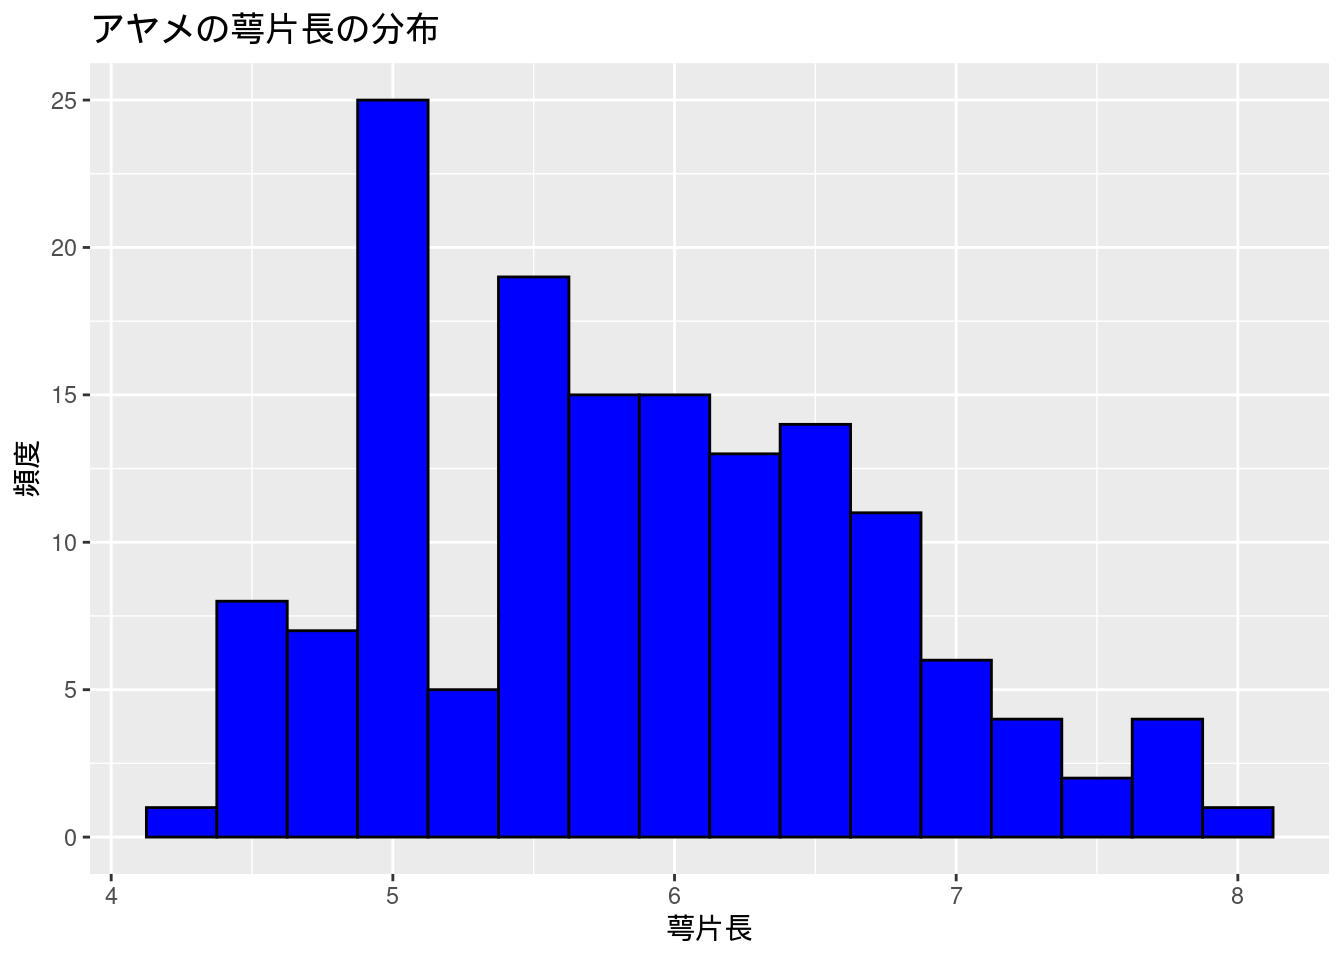
\includegraphics{_main_files/figure-latex/unnamed-chunk-41-1.pdf}

ここでは,IPAexGothicフォントを指定している。もちろん,IPAexGothicフォントがパソコンにインストールされている必要がある。IPAフォントのダウンロードやインストール方法の解説は,\href{https://moji.or.jp/ipafont/}{文字情報技術促進協議会のホームページ}を見てほしい。

theme\_gray()の部分を変更すれば,グラフの見た目を変えることができる。たとえば,theme\_bw()に変えれば,背景が白になるので,印刷する場合に見やすい。

\hypertarget{ux7bb1ux3072ux3052ux56f3}{%
\section{箱ひげ図}\label{ux7bb1ux3072ux3052ux56f3}}

一変数の分布だけに関心があるときにはヒストグラムが有用だが,複数の変数の分布を比較したいときには箱ひげ図が便利である。

まず,アヤメの萼片長の箱ひげ図を描いてみよう。

\begin{Shaded}
\begin{Highlighting}[]
\NormalTok{bp }\OtherTok{\textless{}{-}}\NormalTok{ iris }\SpecialCharTok{\%\textgreater{}\%} 
  \FunctionTok{ggplot}\NormalTok{(}\FunctionTok{aes}\NormalTok{(}\AttributeTok{y=}\NormalTok{Sepal.Length))}\SpecialCharTok{+}
  \FunctionTok{geom\_boxplot}\NormalTok{()}

\FunctionTok{plot}\NormalTok{(bp)}
\end{Highlighting}
\end{Shaded}

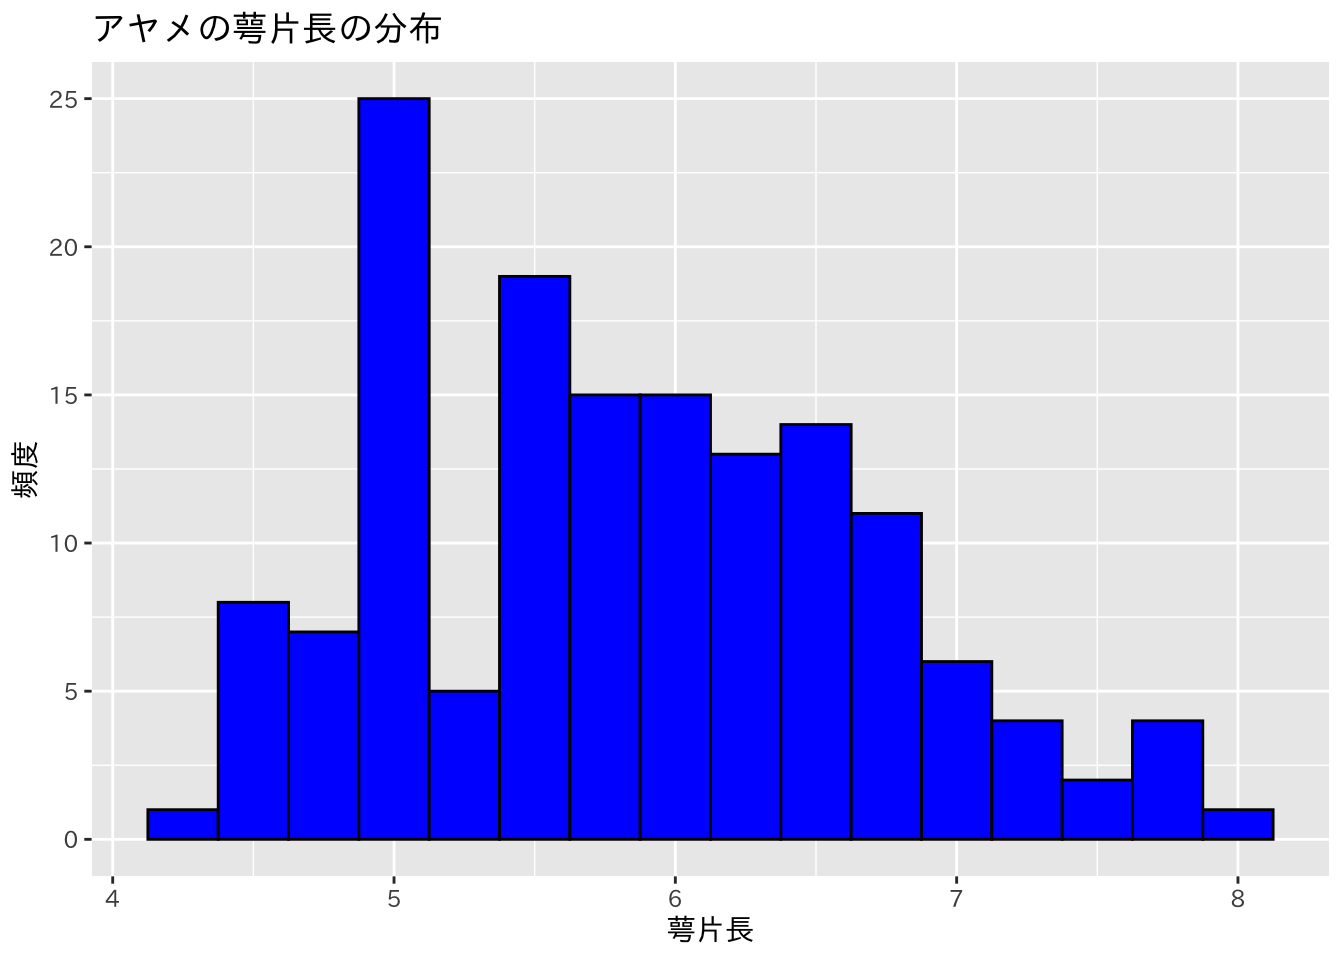
\includegraphics{_main_files/figure-latex/unnamed-chunk-42-1.pdf}

箱ひげ図の場合には,aes()でy軸に変数を指定してやるだけで良い。ここで,yではなくxを指定すれば,横向きの箱ひげ図を描くことができる。

次に,アヤメの種類ごとに箱ひげ図を描いて,萼片長の分布を比較しよう。

\begin{Shaded}
\begin{Highlighting}[]
\NormalTok{bp }\OtherTok{\textless{}{-}}\NormalTok{ iris }\SpecialCharTok{\%\textgreater{}\%} 
  \FunctionTok{ggplot}\NormalTok{(}\FunctionTok{aes}\NormalTok{(}\AttributeTok{y=}\NormalTok{Sepal.Length, }\AttributeTok{fill=}\NormalTok{Species))}\SpecialCharTok{+}
  \FunctionTok{geom\_boxplot}\NormalTok{()}

\FunctionTok{plot}\NormalTok{(bp)}
\end{Highlighting}
\end{Shaded}

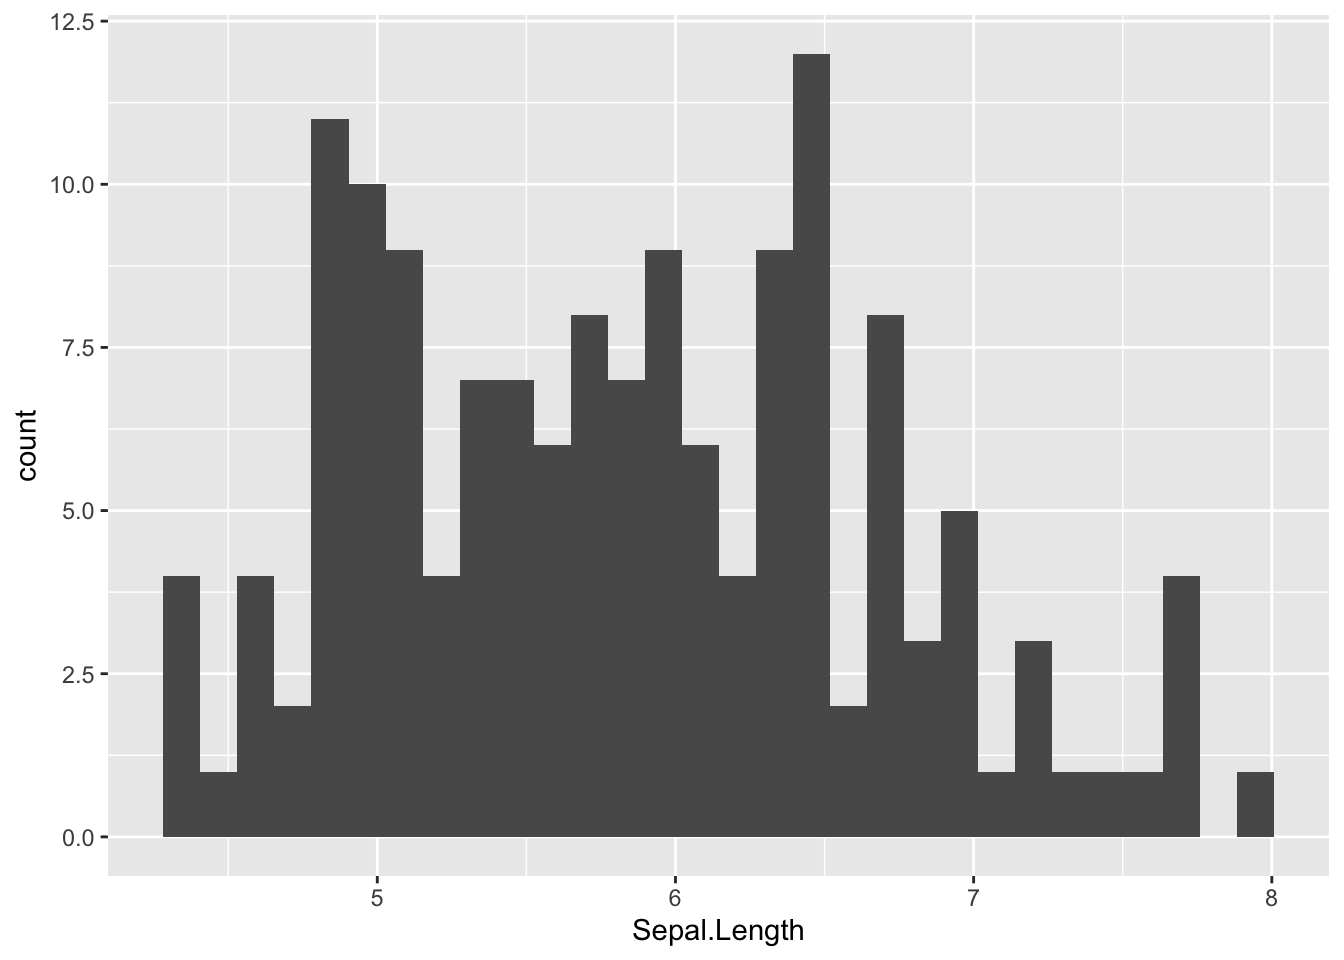
\includegraphics{_main_files/figure-latex/unnamed-chunk-43-1.pdf}

ggplot関数では,aes()にfillでファクター型変数を指定すれば,指定された変数のレベルごとに塗り色を分けてグラフを描くことができる。ここでは,Speciesを指定して,アヤメの種類ごとに塗り分けてグラフを描いている。

\hypertarget{ux6563ux5e03ux56f3}{%
\section{散布図}\label{ux6563ux5e03ux56f3}}

次に,変数の間の関係を分析するために,散布図を作成してみよう。ここでは,アヤメの萼片の長さを横軸に,萼片の幅を縦軸にとって,この二変数の関係を表す散布図を作成する。

\begin{Shaded}
\begin{Highlighting}[]
\NormalTok{scatter }\OtherTok{\textless{}{-}}\NormalTok{ iris }\SpecialCharTok{\%\textgreater{}\%} 
  \FunctionTok{ggplot}\NormalTok{(}\FunctionTok{aes}\NormalTok{(}\AttributeTok{x=}\NormalTok{Sepal.Length, }\AttributeTok{y=}\NormalTok{Sepal.Width))}\SpecialCharTok{+}
  \FunctionTok{geom\_point}\NormalTok{()}

\FunctionTok{plot}\NormalTok{(scatter)}
\end{Highlighting}
\end{Shaded}

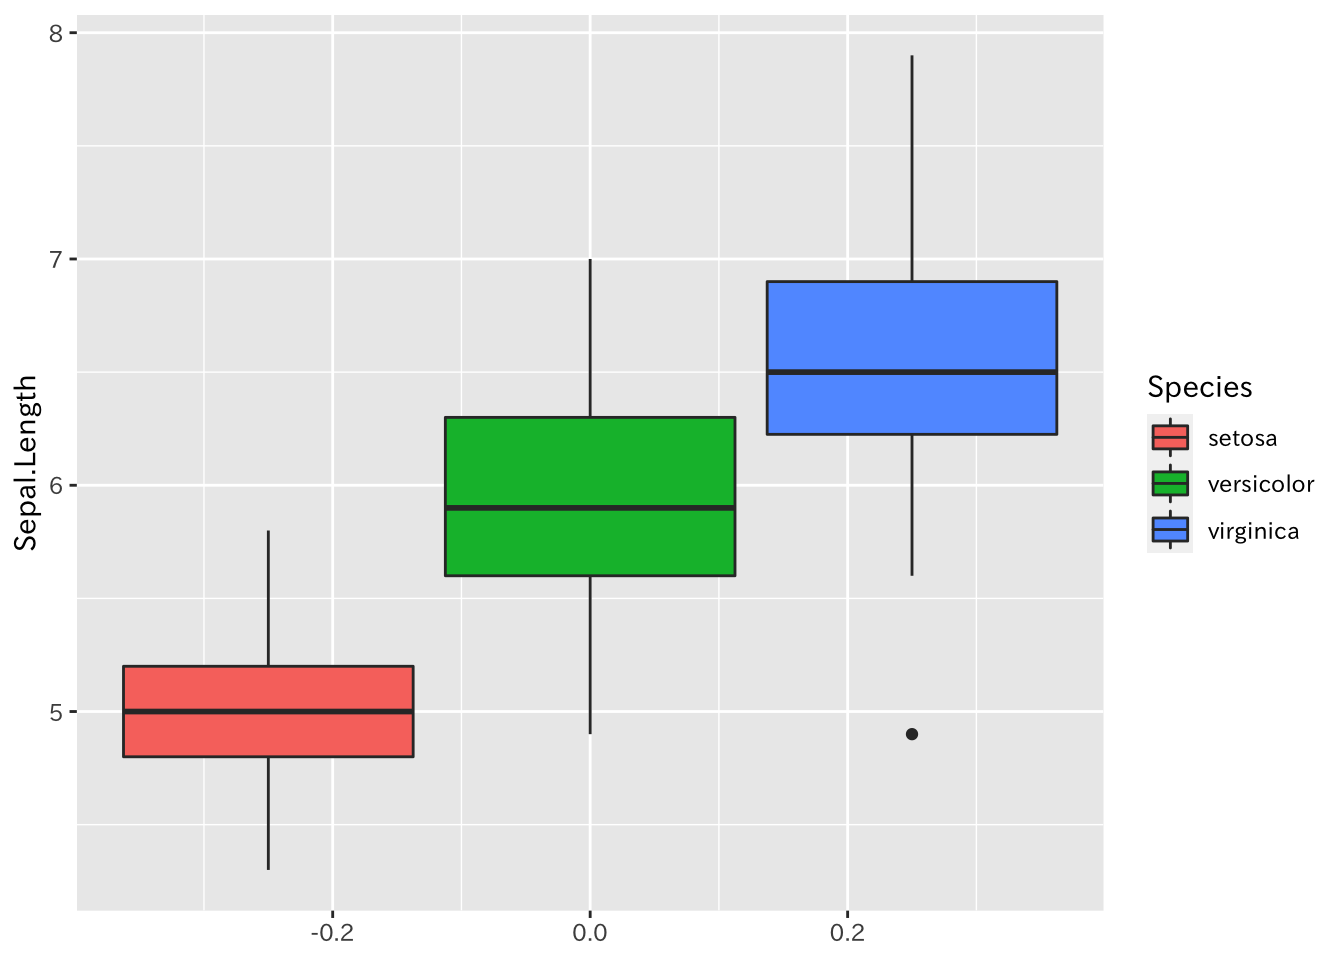
\includegraphics{_main_files/figure-latex/unnamed-chunk-44-1.pdf}

散布図の場合は,aes()でx軸の変数とy軸の変数を指定する。あとは,geom\_point()を足してやれば,単純な散布図を描くことができる。

散布図も,アヤメの種類ごとに色分けして描くことができる。色分けを行うには,aes()のcolorでファクター型変数を指定すれば良い。この場合は,Speciesによって点の色を変えるので,以下のように書く。

\begin{Shaded}
\begin{Highlighting}[]
\NormalTok{scatter }\OtherTok{\textless{}{-}}\NormalTok{ iris }\SpecialCharTok{\%\textgreater{}\%} 
  \FunctionTok{ggplot}\NormalTok{(}\FunctionTok{aes}\NormalTok{(}\AttributeTok{x=}\NormalTok{Sepal.Length, }\AttributeTok{y=}\NormalTok{Sepal.Width, }\AttributeTok{color=}\NormalTok{Species))}\SpecialCharTok{+}
  \FunctionTok{geom\_point}\NormalTok{()}\SpecialCharTok{+}
  \FunctionTok{labs}\NormalTok{(}\AttributeTok{x=}\StringTok{"萼片長"}\NormalTok{,}\AttributeTok{y=}\StringTok{"萼片幅"}\NormalTok{, }\AttributeTok{title=}\StringTok{"萼片の長さと幅の関係"}\NormalTok{)}

\FunctionTok{plot}\NormalTok{(scatter)}
\end{Highlighting}
\end{Shaded}

\begin{verbatim}
## Warning in grid.Call(C_textBounds, as.graphicsAnnot(x$label), x$x, x$y, :
## 'mbcsToSbcs' 中の '萼片幅' で変換に失敗: <e8> をドットで置き換えました
\end{verbatim}

\begin{verbatim}
## Warning in grid.Call(C_textBounds, as.graphicsAnnot(x$label), x$x, x$y, :
## 'mbcsToSbcs' 中の '萼片幅' で変換に失敗: <90> をドットで置き換えました
\end{verbatim}

\begin{verbatim}
## Warning in grid.Call(C_textBounds, as.graphicsAnnot(x$label), x$x, x$y, :
## 'mbcsToSbcs' 中の '萼片幅' で変換に失敗: <bc> をドットで置き換えました
\end{verbatim}

\begin{verbatim}
## Warning in grid.Call(C_textBounds, as.graphicsAnnot(x$label), x$x, x$y, :
## 'mbcsToSbcs' 中の '萼片幅' で変換に失敗: <e7> をドットで置き換えました
\end{verbatim}

\begin{verbatim}
## Warning in grid.Call(C_textBounds, as.graphicsAnnot(x$label), x$x, x$y, :
## 'mbcsToSbcs' 中の '萼片幅' で変換に失敗: <89> をドットで置き換えました
\end{verbatim}

\begin{verbatim}
## Warning in grid.Call(C_textBounds, as.graphicsAnnot(x$label), x$x, x$y, :
## 'mbcsToSbcs' 中の '萼片幅' で変換に失敗: <87> をドットで置き換えました
\end{verbatim}

\begin{verbatim}
## Warning in grid.Call(C_textBounds, as.graphicsAnnot(x$label), x$x, x$y, :
## 'mbcsToSbcs' 中の '萼片幅' で変換に失敗: <e5> をドットで置き換えました
\end{verbatim}

\begin{verbatim}
## Warning in grid.Call(C_textBounds, as.graphicsAnnot(x$label), x$x, x$y, :
## 'mbcsToSbcs' 中の '萼片幅' で変換に失敗: <b9> をドットで置き換えました
\end{verbatim}

\begin{verbatim}
## Warning in grid.Call(C_textBounds, as.graphicsAnnot(x$label), x$x, x$y, :
## 'mbcsToSbcs' 中の '萼片幅' で変換に失敗: <85> をドットで置き換えました
\end{verbatim}

\begin{verbatim}
## Warning in grid.Call(C_textBounds, as.graphicsAnnot(x$label), x$x, x$y, :
## 'mbcsToSbcs' 中の '萼片幅' で変換に失敗: <e8> をドットで置き換えました
\end{verbatim}

\begin{verbatim}
## Warning in grid.Call(C_textBounds, as.graphicsAnnot(x$label), x$x, x$y, :
## 'mbcsToSbcs' 中の '萼片幅' で変換に失敗: <90> をドットで置き換えました
\end{verbatim}

\begin{verbatim}
## Warning in grid.Call(C_textBounds, as.graphicsAnnot(x$label), x$x, x$y, :
## 'mbcsToSbcs' 中の '萼片幅' で変換に失敗: <bc> をドットで置き換えました
\end{verbatim}

\begin{verbatim}
## Warning in grid.Call(C_textBounds, as.graphicsAnnot(x$label), x$x, x$y, :
## 'mbcsToSbcs' 中の '萼片幅' で変換に失敗: <e7> をドットで置き換えました
\end{verbatim}

\begin{verbatim}
## Warning in grid.Call(C_textBounds, as.graphicsAnnot(x$label), x$x, x$y, :
## 'mbcsToSbcs' 中の '萼片幅' で変換に失敗: <89> をドットで置き換えました
\end{verbatim}

\begin{verbatim}
## Warning in grid.Call(C_textBounds, as.graphicsAnnot(x$label), x$x, x$y, :
## 'mbcsToSbcs' 中の '萼片幅' で変換に失敗: <87> をドットで置き換えました
\end{verbatim}

\begin{verbatim}
## Warning in grid.Call(C_textBounds, as.graphicsAnnot(x$label), x$x, x$y, :
## 'mbcsToSbcs' 中の '萼片幅' で変換に失敗: <e5> をドットで置き換えました
\end{verbatim}

\begin{verbatim}
## Warning in grid.Call(C_textBounds, as.graphicsAnnot(x$label), x$x, x$y, :
## 'mbcsToSbcs' 中の '萼片幅' で変換に失敗: <b9> をドットで置き換えました
\end{verbatim}

\begin{verbatim}
## Warning in grid.Call(C_textBounds, as.graphicsAnnot(x$label), x$x, x$y, :
## 'mbcsToSbcs' 中の '萼片幅' で変換に失敗: <85> をドットで置き換えました
\end{verbatim}

\begin{verbatim}
## Warning in grid.Call(C_textBounds, as.graphicsAnnot(x$label), x$x, x$y, :
## 'mbcsToSbcs' 中の '萼片の長さと幅の関係' で変換に失敗: <e8> をドットで置き換えま
## した
\end{verbatim}

\begin{verbatim}
## Warning in grid.Call(C_textBounds, as.graphicsAnnot(x$label), x$x, x$y, :
## 'mbcsToSbcs' 中の '萼片の長さと幅の関係' で変換に失敗: <90> をドットで置き換えま
## した
\end{verbatim}

\begin{verbatim}
## Warning in grid.Call(C_textBounds, as.graphicsAnnot(x$label), x$x, x$y, :
## 'mbcsToSbcs' 中の '萼片の長さと幅の関係' で変換に失敗: <bc> をドットで置き換えま
## した
\end{verbatim}

\begin{verbatim}
## Warning in grid.Call(C_textBounds, as.graphicsAnnot(x$label), x$x, x$y, :
## 'mbcsToSbcs' 中の '萼片の長さと幅の関係' で変換に失敗: <e7> をドットで置き換えま
## した
\end{verbatim}

\begin{verbatim}
## Warning in grid.Call(C_textBounds, as.graphicsAnnot(x$label), x$x, x$y, :
## 'mbcsToSbcs' 中の '萼片の長さと幅の関係' で変換に失敗: <89> をドットで置き換えま
## した
\end{verbatim}

\begin{verbatim}
## Warning in grid.Call(C_textBounds, as.graphicsAnnot(x$label), x$x, x$y, :
## 'mbcsToSbcs' 中の '萼片の長さと幅の関係' で変換に失敗: <87> をドットで置き換えま
## した
\end{verbatim}

\begin{verbatim}
## Warning in grid.Call(C_textBounds, as.graphicsAnnot(x$label), x$x, x$y, :
## 'mbcsToSbcs' 中の '萼片の長さと幅の関係' で変換に失敗: <e3> をドットで置き換えま
## した
\end{verbatim}

\begin{verbatim}
## Warning in grid.Call(C_textBounds, as.graphicsAnnot(x$label), x$x, x$y, :
## 'mbcsToSbcs' 中の '萼片の長さと幅の関係' で変換に失敗: <81> をドットで置き換えま
## した
\end{verbatim}

\begin{verbatim}
## Warning in grid.Call(C_textBounds, as.graphicsAnnot(x$label), x$x, x$y, :
## 'mbcsToSbcs' 中の '萼片の長さと幅の関係' で変換に失敗: <ae> をドットで置き換えま
## した
\end{verbatim}

\begin{verbatim}
## Warning in grid.Call(C_textBounds, as.graphicsAnnot(x$label), x$x, x$y, :
## 'mbcsToSbcs' 中の '萼片の長さと幅の関係' で変換に失敗: <e9> をドットで置き換えま
## した
\end{verbatim}

\begin{verbatim}
## Warning in grid.Call(C_textBounds, as.graphicsAnnot(x$label), x$x, x$y, :
## 'mbcsToSbcs' 中の '萼片の長さと幅の関係' で変換に失敗: <95> をドットで置き換えま
## した
\end{verbatim}

\begin{verbatim}
## Warning in grid.Call(C_textBounds, as.graphicsAnnot(x$label), x$x, x$y, :
## 'mbcsToSbcs' 中の '萼片の長さと幅の関係' で変換に失敗: <b7> をドットで置き換えま
## した
\end{verbatim}

\begin{verbatim}
## Warning in grid.Call(C_textBounds, as.graphicsAnnot(x$label), x$x, x$y, :
## 'mbcsToSbcs' 中の '萼片の長さと幅の関係' で変換に失敗: <e3> をドットで置き換えま
## した
\end{verbatim}

\begin{verbatim}
## Warning in grid.Call(C_textBounds, as.graphicsAnnot(x$label), x$x, x$y, :
## 'mbcsToSbcs' 中の '萼片の長さと幅の関係' で変換に失敗: <81> をドットで置き換えま
## した
\end{verbatim}

\begin{verbatim}
## Warning in grid.Call(C_textBounds, as.graphicsAnnot(x$label), x$x, x$y, :
## 'mbcsToSbcs' 中の '萼片の長さと幅の関係' で変換に失敗: <95> をドットで置き換えま
## した
\end{verbatim}

\begin{verbatim}
## Warning in grid.Call(C_textBounds, as.graphicsAnnot(x$label), x$x, x$y, :
## 'mbcsToSbcs' 中の '萼片の長さと幅の関係' で変換に失敗: <e3> をドットで置き換えま
## した
\end{verbatim}

\begin{verbatim}
## Warning in grid.Call(C_textBounds, as.graphicsAnnot(x$label), x$x, x$y, :
## 'mbcsToSbcs' 中の '萼片の長さと幅の関係' で変換に失敗: <81> をドットで置き換えま
## した
\end{verbatim}

\begin{verbatim}
## Warning in grid.Call(C_textBounds, as.graphicsAnnot(x$label), x$x, x$y, :
## 'mbcsToSbcs' 中の '萼片の長さと幅の関係' で変換に失敗: <a8> をドットで置き換えま
## した
\end{verbatim}

\begin{verbatim}
## Warning in grid.Call(C_textBounds, as.graphicsAnnot(x$label), x$x, x$y, :
## 'mbcsToSbcs' 中の '萼片の長さと幅の関係' で変換に失敗: <e5> をドットで置き換えま
## した
\end{verbatim}

\begin{verbatim}
## Warning in grid.Call(C_textBounds, as.graphicsAnnot(x$label), x$x, x$y, :
## 'mbcsToSbcs' 中の '萼片の長さと幅の関係' で変換に失敗: <b9> をドットで置き換えま
## した
\end{verbatim}

\begin{verbatim}
## Warning in grid.Call(C_textBounds, as.graphicsAnnot(x$label), x$x, x$y, :
## 'mbcsToSbcs' 中の '萼片の長さと幅の関係' で変換に失敗: <85> をドットで置き換えま
## した
\end{verbatim}

\begin{verbatim}
## Warning in grid.Call(C_textBounds, as.graphicsAnnot(x$label), x$x, x$y, :
## 'mbcsToSbcs' 中の '萼片の長さと幅の関係' で変換に失敗: <e3> をドットで置き換えま
## した
\end{verbatim}

\begin{verbatim}
## Warning in grid.Call(C_textBounds, as.graphicsAnnot(x$label), x$x, x$y, :
## 'mbcsToSbcs' 中の '萼片の長さと幅の関係' で変換に失敗: <81> をドットで置き換えま
## した
\end{verbatim}

\begin{verbatim}
## Warning in grid.Call(C_textBounds, as.graphicsAnnot(x$label), x$x, x$y, :
## 'mbcsToSbcs' 中の '萼片の長さと幅の関係' で変換に失敗: <ae> をドットで置き換えま
## した
\end{verbatim}

\begin{verbatim}
## Warning in grid.Call(C_textBounds, as.graphicsAnnot(x$label), x$x, x$y, :
## 'mbcsToSbcs' 中の '萼片の長さと幅の関係' で変換に失敗: <e9> をドットで置き換えま
## した
\end{verbatim}

\begin{verbatim}
## Warning in grid.Call(C_textBounds, as.graphicsAnnot(x$label), x$x, x$y, :
## 'mbcsToSbcs' 中の '萼片の長さと幅の関係' で変換に失敗: <96> をドットで置き換えま
## した
\end{verbatim}

\begin{verbatim}
## Warning in grid.Call(C_textBounds, as.graphicsAnnot(x$label), x$x, x$y, :
## 'mbcsToSbcs' 中の '萼片の長さと幅の関係' で変換に失敗: <a2> をドットで置き換えま
## した
\end{verbatim}

\begin{verbatim}
## Warning in grid.Call(C_textBounds, as.graphicsAnnot(x$label), x$x, x$y, :
## 'mbcsToSbcs' 中の '萼片の長さと幅の関係' で変換に失敗: <e4> をドットで置き換えま
## した
\end{verbatim}

\begin{verbatim}
## Warning in grid.Call(C_textBounds, as.graphicsAnnot(x$label), x$x, x$y, :
## 'mbcsToSbcs' 中の '萼片の長さと幅の関係' で変換に失敗: <bf> をドットで置き換えま
## した
\end{verbatim}

\begin{verbatim}
## Warning in grid.Call(C_textBounds, as.graphicsAnnot(x$label), x$x, x$y, :
## 'mbcsToSbcs' 中の '萼片の長さと幅の関係' で変換に失敗: <82> をドットで置き換えま
## した
\end{verbatim}

\begin{verbatim}
## Warning in grid.Call(C_textBounds, as.graphicsAnnot(x$label), x$x, x$y, :
## 'mbcsToSbcs' 中の '萼片の長さと幅の関係' で変換に失敗: <e8> をドットで置き換えま
## した
\end{verbatim}

\begin{verbatim}
## Warning in grid.Call(C_textBounds, as.graphicsAnnot(x$label), x$x, x$y, :
## 'mbcsToSbcs' 中の '萼片の長さと幅の関係' で変換に失敗: <90> をドットで置き換えま
## した
\end{verbatim}

\begin{verbatim}
## Warning in grid.Call(C_textBounds, as.graphicsAnnot(x$label), x$x, x$y, :
## 'mbcsToSbcs' 中の '萼片の長さと幅の関係' で変換に失敗: <bc> をドットで置き換えま
## した
\end{verbatim}

\begin{verbatim}
## Warning in grid.Call(C_textBounds, as.graphicsAnnot(x$label), x$x, x$y, :
## 'mbcsToSbcs' 中の '萼片の長さと幅の関係' で変換に失敗: <e7> をドットで置き換えま
## した
\end{verbatim}

\begin{verbatim}
## Warning in grid.Call(C_textBounds, as.graphicsAnnot(x$label), x$x, x$y, :
## 'mbcsToSbcs' 中の '萼片の長さと幅の関係' で変換に失敗: <89> をドットで置き換えま
## した
\end{verbatim}

\begin{verbatim}
## Warning in grid.Call(C_textBounds, as.graphicsAnnot(x$label), x$x, x$y, :
## 'mbcsToSbcs' 中の '萼片の長さと幅の関係' で変換に失敗: <87> をドットで置き換えま
## した
\end{verbatim}

\begin{verbatim}
## Warning in grid.Call(C_textBounds, as.graphicsAnnot(x$label), x$x, x$y, :
## 'mbcsToSbcs' 中の '萼片の長さと幅の関係' で変換に失敗: <e3> をドットで置き換えま
## した
\end{verbatim}

\begin{verbatim}
## Warning in grid.Call(C_textBounds, as.graphicsAnnot(x$label), x$x, x$y, :
## 'mbcsToSbcs' 中の '萼片の長さと幅の関係' で変換に失敗: <81> をドットで置き換えま
## した
\end{verbatim}

\begin{verbatim}
## Warning in grid.Call(C_textBounds, as.graphicsAnnot(x$label), x$x, x$y, :
## 'mbcsToSbcs' 中の '萼片の長さと幅の関係' で変換に失敗: <ae> をドットで置き換えま
## した
\end{verbatim}

\begin{verbatim}
## Warning in grid.Call(C_textBounds, as.graphicsAnnot(x$label), x$x, x$y, :
## 'mbcsToSbcs' 中の '萼片の長さと幅の関係' で変換に失敗: <e9> をドットで置き換えま
## した
\end{verbatim}

\begin{verbatim}
## Warning in grid.Call(C_textBounds, as.graphicsAnnot(x$label), x$x, x$y, :
## 'mbcsToSbcs' 中の '萼片の長さと幅の関係' で変換に失敗: <95> をドットで置き換えま
## した
\end{verbatim}

\begin{verbatim}
## Warning in grid.Call(C_textBounds, as.graphicsAnnot(x$label), x$x, x$y, :
## 'mbcsToSbcs' 中の '萼片の長さと幅の関係' で変換に失敗: <b7> をドットで置き換えま
## した
\end{verbatim}

\begin{verbatim}
## Warning in grid.Call(C_textBounds, as.graphicsAnnot(x$label), x$x, x$y, :
## 'mbcsToSbcs' 中の '萼片の長さと幅の関係' で変換に失敗: <e3> をドットで置き換えま
## した
\end{verbatim}

\begin{verbatim}
## Warning in grid.Call(C_textBounds, as.graphicsAnnot(x$label), x$x, x$y, :
## 'mbcsToSbcs' 中の '萼片の長さと幅の関係' で変換に失敗: <81> をドットで置き換えま
## した
\end{verbatim}

\begin{verbatim}
## Warning in grid.Call(C_textBounds, as.graphicsAnnot(x$label), x$x, x$y, :
## 'mbcsToSbcs' 中の '萼片の長さと幅の関係' で変換に失敗: <95> をドットで置き換えま
## した
\end{verbatim}

\begin{verbatim}
## Warning in grid.Call(C_textBounds, as.graphicsAnnot(x$label), x$x, x$y, :
## 'mbcsToSbcs' 中の '萼片の長さと幅の関係' で変換に失敗: <e3> をドットで置き換えま
## した
\end{verbatim}

\begin{verbatim}
## Warning in grid.Call(C_textBounds, as.graphicsAnnot(x$label), x$x, x$y, :
## 'mbcsToSbcs' 中の '萼片の長さと幅の関係' で変換に失敗: <81> をドットで置き換えま
## した
\end{verbatim}

\begin{verbatim}
## Warning in grid.Call(C_textBounds, as.graphicsAnnot(x$label), x$x, x$y, :
## 'mbcsToSbcs' 中の '萼片の長さと幅の関係' で変換に失敗: <a8> をドットで置き換えま
## した
\end{verbatim}

\begin{verbatim}
## Warning in grid.Call(C_textBounds, as.graphicsAnnot(x$label), x$x, x$y, :
## 'mbcsToSbcs' 中の '萼片の長さと幅の関係' で変換に失敗: <e5> をドットで置き換えま
## した
\end{verbatim}

\begin{verbatim}
## Warning in grid.Call(C_textBounds, as.graphicsAnnot(x$label), x$x, x$y, :
## 'mbcsToSbcs' 中の '萼片の長さと幅の関係' で変換に失敗: <b9> をドットで置き換えま
## した
\end{verbatim}

\begin{verbatim}
## Warning in grid.Call(C_textBounds, as.graphicsAnnot(x$label), x$x, x$y, :
## 'mbcsToSbcs' 中の '萼片の長さと幅の関係' で変換に失敗: <85> をドットで置き換えま
## した
\end{verbatim}

\begin{verbatim}
## Warning in grid.Call(C_textBounds, as.graphicsAnnot(x$label), x$x, x$y, :
## 'mbcsToSbcs' 中の '萼片の長さと幅の関係' で変換に失敗: <e3> をドットで置き換えま
## した
\end{verbatim}

\begin{verbatim}
## Warning in grid.Call(C_textBounds, as.graphicsAnnot(x$label), x$x, x$y, :
## 'mbcsToSbcs' 中の '萼片の長さと幅の関係' で変換に失敗: <81> をドットで置き換えま
## した
\end{verbatim}

\begin{verbatim}
## Warning in grid.Call(C_textBounds, as.graphicsAnnot(x$label), x$x, x$y, :
## 'mbcsToSbcs' 中の '萼片の長さと幅の関係' で変換に失敗: <ae> をドットで置き換えま
## した
\end{verbatim}

\begin{verbatim}
## Warning in grid.Call(C_textBounds, as.graphicsAnnot(x$label), x$x, x$y, :
## 'mbcsToSbcs' 中の '萼片の長さと幅の関係' で変換に失敗: <e9> をドットで置き換えま
## した
\end{verbatim}

\begin{verbatim}
## Warning in grid.Call(C_textBounds, as.graphicsAnnot(x$label), x$x, x$y, :
## 'mbcsToSbcs' 中の '萼片の長さと幅の関係' で変換に失敗: <96> をドットで置き換えま
## した
\end{verbatim}

\begin{verbatim}
## Warning in grid.Call(C_textBounds, as.graphicsAnnot(x$label), x$x, x$y, :
## 'mbcsToSbcs' 中の '萼片の長さと幅の関係' で変換に失敗: <a2> をドットで置き換えま
## した
\end{verbatim}

\begin{verbatim}
## Warning in grid.Call(C_textBounds, as.graphicsAnnot(x$label), x$x, x$y, :
## 'mbcsToSbcs' 中の '萼片の長さと幅の関係' で変換に失敗: <e4> をドットで置き換えま
## した
\end{verbatim}

\begin{verbatim}
## Warning in grid.Call(C_textBounds, as.graphicsAnnot(x$label), x$x, x$y, :
## 'mbcsToSbcs' 中の '萼片の長さと幅の関係' で変換に失敗: <bf> をドットで置き換えま
## した
\end{verbatim}

\begin{verbatim}
## Warning in grid.Call(C_textBounds, as.graphicsAnnot(x$label), x$x, x$y, :
## 'mbcsToSbcs' 中の '萼片の長さと幅の関係' で変換に失敗: <82> をドットで置き換えま
## した
\end{verbatim}

\begin{verbatim}
## Warning in grid.Call(C_textBounds, as.graphicsAnnot(x$label), x$x, x$y, :
## 'mbcsToSbcs' 中の '萼片長' で変換に失敗: <e8> をドットで置き換えました
\end{verbatim}

\begin{verbatim}
## Warning in grid.Call(C_textBounds, as.graphicsAnnot(x$label), x$x, x$y, :
## 'mbcsToSbcs' 中の '萼片長' で変換に失敗: <90> をドットで置き換えました
\end{verbatim}

\begin{verbatim}
## Warning in grid.Call(C_textBounds, as.graphicsAnnot(x$label), x$x, x$y, :
## 'mbcsToSbcs' 中の '萼片長' で変換に失敗: <bc> をドットで置き換えました
\end{verbatim}

\begin{verbatim}
## Warning in grid.Call(C_textBounds, as.graphicsAnnot(x$label), x$x, x$y, :
## 'mbcsToSbcs' 中の '萼片長' で変換に失敗: <e7> をドットで置き換えました
\end{verbatim}

\begin{verbatim}
## Warning in grid.Call(C_textBounds, as.graphicsAnnot(x$label), x$x, x$y, :
## 'mbcsToSbcs' 中の '萼片長' で変換に失敗: <89> をドットで置き換えました
\end{verbatim}

\begin{verbatim}
## Warning in grid.Call(C_textBounds, as.graphicsAnnot(x$label), x$x, x$y, :
## 'mbcsToSbcs' 中の '萼片長' で変換に失敗: <87> をドットで置き換えました
\end{verbatim}

\begin{verbatim}
## Warning in grid.Call(C_textBounds, as.graphicsAnnot(x$label), x$x, x$y, :
## 'mbcsToSbcs' 中の '萼片長' で変換に失敗: <e9> をドットで置き換えました
\end{verbatim}

\begin{verbatim}
## Warning in grid.Call(C_textBounds, as.graphicsAnnot(x$label), x$x, x$y, :
## 'mbcsToSbcs' 中の '萼片長' で変換に失敗: <95> をドットで置き換えました
\end{verbatim}

\begin{verbatim}
## Warning in grid.Call(C_textBounds, as.graphicsAnnot(x$label), x$x, x$y, :
## 'mbcsToSbcs' 中の '萼片長' で変換に失敗: <b7> をドットで置き換えました
\end{verbatim}

\begin{verbatim}
## Warning in grid.Call(C_textBounds, as.graphicsAnnot(x$label), x$x, x$y, :
## 'mbcsToSbcs' 中の '萼片長' で変換に失敗: <e8> をドットで置き換えました
\end{verbatim}

\begin{verbatim}
## Warning in grid.Call(C_textBounds, as.graphicsAnnot(x$label), x$x, x$y, :
## 'mbcsToSbcs' 中の '萼片長' で変換に失敗: <90> をドットで置き換えました
\end{verbatim}

\begin{verbatim}
## Warning in grid.Call(C_textBounds, as.graphicsAnnot(x$label), x$x, x$y, :
## 'mbcsToSbcs' 中の '萼片長' で変換に失敗: <bc> をドットで置き換えました
\end{verbatim}

\begin{verbatim}
## Warning in grid.Call(C_textBounds, as.graphicsAnnot(x$label), x$x, x$y, :
## 'mbcsToSbcs' 中の '萼片長' で変換に失敗: <e7> をドットで置き換えました
\end{verbatim}

\begin{verbatim}
## Warning in grid.Call(C_textBounds, as.graphicsAnnot(x$label), x$x, x$y, :
## 'mbcsToSbcs' 中の '萼片長' で変換に失敗: <89> をドットで置き換えました
\end{verbatim}

\begin{verbatim}
## Warning in grid.Call(C_textBounds, as.graphicsAnnot(x$label), x$x, x$y, :
## 'mbcsToSbcs' 中の '萼片長' で変換に失敗: <87> をドットで置き換えました
\end{verbatim}

\begin{verbatim}
## Warning in grid.Call(C_textBounds, as.graphicsAnnot(x$label), x$x, x$y, :
## 'mbcsToSbcs' 中の '萼片長' で変換に失敗: <e9> をドットで置き換えました
\end{verbatim}

\begin{verbatim}
## Warning in grid.Call(C_textBounds, as.graphicsAnnot(x$label), x$x, x$y, :
## 'mbcsToSbcs' 中の '萼片長' で変換に失敗: <95> をドットで置き換えました
\end{verbatim}

\begin{verbatim}
## Warning in grid.Call(C_textBounds, as.graphicsAnnot(x$label), x$x, x$y, :
## 'mbcsToSbcs' 中の '萼片長' で変換に失敗: <b7> をドットで置き換えました
\end{verbatim}

\begin{verbatim}
## Warning in grid.Call(C_textBounds, as.graphicsAnnot(x$label), x$x, x$y, :
## 'mbcsToSbcs' 中の '萼片幅' で変換に失敗: <e8> をドットで置き換えました
\end{verbatim}

\begin{verbatim}
## Warning in grid.Call(C_textBounds, as.graphicsAnnot(x$label), x$x, x$y, :
## 'mbcsToSbcs' 中の '萼片幅' で変換に失敗: <90> をドットで置き換えました
\end{verbatim}

\begin{verbatim}
## Warning in grid.Call(C_textBounds, as.graphicsAnnot(x$label), x$x, x$y, :
## 'mbcsToSbcs' 中の '萼片幅' で変換に失敗: <bc> をドットで置き換えました
\end{verbatim}

\begin{verbatim}
## Warning in grid.Call(C_textBounds, as.graphicsAnnot(x$label), x$x, x$y, :
## 'mbcsToSbcs' 中の '萼片幅' で変換に失敗: <e7> をドットで置き換えました
\end{verbatim}

\begin{verbatim}
## Warning in grid.Call(C_textBounds, as.graphicsAnnot(x$label), x$x, x$y, :
## 'mbcsToSbcs' 中の '萼片幅' で変換に失敗: <89> をドットで置き換えました
\end{verbatim}

\begin{verbatim}
## Warning in grid.Call(C_textBounds, as.graphicsAnnot(x$label), x$x, x$y, :
## 'mbcsToSbcs' 中の '萼片幅' で変換に失敗: <87> をドットで置き換えました
\end{verbatim}

\begin{verbatim}
## Warning in grid.Call(C_textBounds, as.graphicsAnnot(x$label), x$x, x$y, :
## 'mbcsToSbcs' 中の '萼片幅' で変換に失敗: <e5> をドットで置き換えました
\end{verbatim}

\begin{verbatim}
## Warning in grid.Call(C_textBounds, as.graphicsAnnot(x$label), x$x, x$y, :
## 'mbcsToSbcs' 中の '萼片幅' で変換に失敗: <b9> をドットで置き換えました
\end{verbatim}

\begin{verbatim}
## Warning in grid.Call(C_textBounds, as.graphicsAnnot(x$label), x$x, x$y, :
## 'mbcsToSbcs' 中の '萼片幅' で変換に失敗: <85> をドットで置き換えました
\end{verbatim}

\begin{verbatim}
## Warning in grid.Call(C_textBounds, as.graphicsAnnot(x$label), x$x, x$y, :
## 'mbcsToSbcs' 中の '萼片幅' で変換に失敗: <e8> をドットで置き換えました
\end{verbatim}

\begin{verbatim}
## Warning in grid.Call(C_textBounds, as.graphicsAnnot(x$label), x$x, x$y, :
## 'mbcsToSbcs' 中の '萼片幅' で変換に失敗: <90> をドットで置き換えました
\end{verbatim}

\begin{verbatim}
## Warning in grid.Call(C_textBounds, as.graphicsAnnot(x$label), x$x, x$y, :
## 'mbcsToSbcs' 中の '萼片幅' で変換に失敗: <bc> をドットで置き換えました
\end{verbatim}

\begin{verbatim}
## Warning in grid.Call(C_textBounds, as.graphicsAnnot(x$label), x$x, x$y, :
## 'mbcsToSbcs' 中の '萼片幅' で変換に失敗: <e7> をドットで置き換えました
\end{verbatim}

\begin{verbatim}
## Warning in grid.Call(C_textBounds, as.graphicsAnnot(x$label), x$x, x$y, :
## 'mbcsToSbcs' 中の '萼片幅' で変換に失敗: <89> をドットで置き換えました
\end{verbatim}

\begin{verbatim}
## Warning in grid.Call(C_textBounds, as.graphicsAnnot(x$label), x$x, x$y, :
## 'mbcsToSbcs' 中の '萼片幅' で変換に失敗: <87> をドットで置き換えました
\end{verbatim}

\begin{verbatim}
## Warning in grid.Call(C_textBounds, as.graphicsAnnot(x$label), x$x, x$y, :
## 'mbcsToSbcs' 中の '萼片幅' で変換に失敗: <e5> をドットで置き換えました
\end{verbatim}

\begin{verbatim}
## Warning in grid.Call(C_textBounds, as.graphicsAnnot(x$label), x$x, x$y, :
## 'mbcsToSbcs' 中の '萼片幅' で変換に失敗: <b9> をドットで置き換えました
\end{verbatim}

\begin{verbatim}
## Warning in grid.Call(C_textBounds, as.graphicsAnnot(x$label), x$x, x$y, :
## 'mbcsToSbcs' 中の '萼片幅' で変換に失敗: <85> をドットで置き換えました
\end{verbatim}

\begin{verbatim}
## Warning in grid.Call(C_textBounds, as.graphicsAnnot(x$label), x$x, x$y, :
## 'mbcsToSbcs' 中の '萼片幅' で変換に失敗: <e8> をドットで置き換えました
\end{verbatim}

\begin{verbatim}
## Warning in grid.Call(C_textBounds, as.graphicsAnnot(x$label), x$x, x$y, :
## 'mbcsToSbcs' 中の '萼片幅' で変換に失敗: <90> をドットで置き換えました
\end{verbatim}

\begin{verbatim}
## Warning in grid.Call(C_textBounds, as.graphicsAnnot(x$label), x$x, x$y, :
## 'mbcsToSbcs' 中の '萼片幅' で変換に失敗: <bc> をドットで置き換えました
\end{verbatim}

\begin{verbatim}
## Warning in grid.Call(C_textBounds, as.graphicsAnnot(x$label), x$x, x$y, :
## 'mbcsToSbcs' 中の '萼片幅' で変換に失敗: <e7> をドットで置き換えました
\end{verbatim}

\begin{verbatim}
## Warning in grid.Call(C_textBounds, as.graphicsAnnot(x$label), x$x, x$y, :
## 'mbcsToSbcs' 中の '萼片幅' で変換に失敗: <89> をドットで置き換えました
\end{verbatim}

\begin{verbatim}
## Warning in grid.Call(C_textBounds, as.graphicsAnnot(x$label), x$x, x$y, :
## 'mbcsToSbcs' 中の '萼片幅' で変換に失敗: <87> をドットで置き換えました
\end{verbatim}

\begin{verbatim}
## Warning in grid.Call(C_textBounds, as.graphicsAnnot(x$label), x$x, x$y, :
## 'mbcsToSbcs' 中の '萼片幅' で変換に失敗: <e5> をドットで置き換えました
\end{verbatim}

\begin{verbatim}
## Warning in grid.Call(C_textBounds, as.graphicsAnnot(x$label), x$x, x$y, :
## 'mbcsToSbcs' 中の '萼片幅' で変換に失敗: <b9> をドットで置き換えました
\end{verbatim}

\begin{verbatim}
## Warning in grid.Call(C_textBounds, as.graphicsAnnot(x$label), x$x, x$y, :
## 'mbcsToSbcs' 中の '萼片幅' で変換に失敗: <85> をドットで置き換えました
\end{verbatim}

\begin{verbatim}
## Warning in grid.Call(C_textBounds, as.graphicsAnnot(x$label), x$x, x$y, :
## 'mbcsToSbcs' 中の '萼片の長さと幅の関係' で変換に失敗: <e8> をドットで置き換えま
## した
\end{verbatim}

\begin{verbatim}
## Warning in grid.Call(C_textBounds, as.graphicsAnnot(x$label), x$x, x$y, :
## 'mbcsToSbcs' 中の '萼片の長さと幅の関係' で変換に失敗: <90> をドットで置き換えま
## した
\end{verbatim}

\begin{verbatim}
## Warning in grid.Call(C_textBounds, as.graphicsAnnot(x$label), x$x, x$y, :
## 'mbcsToSbcs' 中の '萼片の長さと幅の関係' で変換に失敗: <bc> をドットで置き換えま
## した
\end{verbatim}

\begin{verbatim}
## Warning in grid.Call(C_textBounds, as.graphicsAnnot(x$label), x$x, x$y, :
## 'mbcsToSbcs' 中の '萼片の長さと幅の関係' で変換に失敗: <e7> をドットで置き換えま
## した
\end{verbatim}

\begin{verbatim}
## Warning in grid.Call(C_textBounds, as.graphicsAnnot(x$label), x$x, x$y, :
## 'mbcsToSbcs' 中の '萼片の長さと幅の関係' で変換に失敗: <89> をドットで置き換えま
## した
\end{verbatim}

\begin{verbatim}
## Warning in grid.Call(C_textBounds, as.graphicsAnnot(x$label), x$x, x$y, :
## 'mbcsToSbcs' 中の '萼片の長さと幅の関係' で変換に失敗: <87> をドットで置き換えま
## した
\end{verbatim}

\begin{verbatim}
## Warning in grid.Call(C_textBounds, as.graphicsAnnot(x$label), x$x, x$y, :
## 'mbcsToSbcs' 中の '萼片の長さと幅の関係' で変換に失敗: <e3> をドットで置き換えま
## した
\end{verbatim}

\begin{verbatim}
## Warning in grid.Call(C_textBounds, as.graphicsAnnot(x$label), x$x, x$y, :
## 'mbcsToSbcs' 中の '萼片の長さと幅の関係' で変換に失敗: <81> をドットで置き換えま
## した
\end{verbatim}

\begin{verbatim}
## Warning in grid.Call(C_textBounds, as.graphicsAnnot(x$label), x$x, x$y, :
## 'mbcsToSbcs' 中の '萼片の長さと幅の関係' で変換に失敗: <ae> をドットで置き換えま
## した
\end{verbatim}

\begin{verbatim}
## Warning in grid.Call(C_textBounds, as.graphicsAnnot(x$label), x$x, x$y, :
## 'mbcsToSbcs' 中の '萼片の長さと幅の関係' で変換に失敗: <e9> をドットで置き換えま
## した
\end{verbatim}

\begin{verbatim}
## Warning in grid.Call(C_textBounds, as.graphicsAnnot(x$label), x$x, x$y, :
## 'mbcsToSbcs' 中の '萼片の長さと幅の関係' で変換に失敗: <95> をドットで置き換えま
## した
\end{verbatim}

\begin{verbatim}
## Warning in grid.Call(C_textBounds, as.graphicsAnnot(x$label), x$x, x$y, :
## 'mbcsToSbcs' 中の '萼片の長さと幅の関係' で変換に失敗: <b7> をドットで置き換えま
## した
\end{verbatim}

\begin{verbatim}
## Warning in grid.Call(C_textBounds, as.graphicsAnnot(x$label), x$x, x$y, :
## 'mbcsToSbcs' 中の '萼片の長さと幅の関係' で変換に失敗: <e3> をドットで置き換えま
## した
\end{verbatim}

\begin{verbatim}
## Warning in grid.Call(C_textBounds, as.graphicsAnnot(x$label), x$x, x$y, :
## 'mbcsToSbcs' 中の '萼片の長さと幅の関係' で変換に失敗: <81> をドットで置き換えま
## した
\end{verbatim}

\begin{verbatim}
## Warning in grid.Call(C_textBounds, as.graphicsAnnot(x$label), x$x, x$y, :
## 'mbcsToSbcs' 中の '萼片の長さと幅の関係' で変換に失敗: <95> をドットで置き換えま
## した
\end{verbatim}

\begin{verbatim}
## Warning in grid.Call(C_textBounds, as.graphicsAnnot(x$label), x$x, x$y, :
## 'mbcsToSbcs' 中の '萼片の長さと幅の関係' で変換に失敗: <e3> をドットで置き換えま
## した
\end{verbatim}

\begin{verbatim}
## Warning in grid.Call(C_textBounds, as.graphicsAnnot(x$label), x$x, x$y, :
## 'mbcsToSbcs' 中の '萼片の長さと幅の関係' で変換に失敗: <81> をドットで置き換えま
## した
\end{verbatim}

\begin{verbatim}
## Warning in grid.Call(C_textBounds, as.graphicsAnnot(x$label), x$x, x$y, :
## 'mbcsToSbcs' 中の '萼片の長さと幅の関係' で変換に失敗: <a8> をドットで置き換えま
## した
\end{verbatim}

\begin{verbatim}
## Warning in grid.Call(C_textBounds, as.graphicsAnnot(x$label), x$x, x$y, :
## 'mbcsToSbcs' 中の '萼片の長さと幅の関係' で変換に失敗: <e5> をドットで置き換えま
## した
\end{verbatim}

\begin{verbatim}
## Warning in grid.Call(C_textBounds, as.graphicsAnnot(x$label), x$x, x$y, :
## 'mbcsToSbcs' 中の '萼片の長さと幅の関係' で変換に失敗: <b9> をドットで置き換えま
## した
\end{verbatim}

\begin{verbatim}
## Warning in grid.Call(C_textBounds, as.graphicsAnnot(x$label), x$x, x$y, :
## 'mbcsToSbcs' 中の '萼片の長さと幅の関係' で変換に失敗: <85> をドットで置き換えま
## した
\end{verbatim}

\begin{verbatim}
## Warning in grid.Call(C_textBounds, as.graphicsAnnot(x$label), x$x, x$y, :
## 'mbcsToSbcs' 中の '萼片の長さと幅の関係' で変換に失敗: <e3> をドットで置き換えま
## した
\end{verbatim}

\begin{verbatim}
## Warning in grid.Call(C_textBounds, as.graphicsAnnot(x$label), x$x, x$y, :
## 'mbcsToSbcs' 中の '萼片の長さと幅の関係' で変換に失敗: <81> をドットで置き換えま
## した
\end{verbatim}

\begin{verbatim}
## Warning in grid.Call(C_textBounds, as.graphicsAnnot(x$label), x$x, x$y, :
## 'mbcsToSbcs' 中の '萼片の長さと幅の関係' で変換に失敗: <ae> をドットで置き換えま
## した
\end{verbatim}

\begin{verbatim}
## Warning in grid.Call(C_textBounds, as.graphicsAnnot(x$label), x$x, x$y, :
## 'mbcsToSbcs' 中の '萼片の長さと幅の関係' で変換に失敗: <e9> をドットで置き換えま
## した
\end{verbatim}

\begin{verbatim}
## Warning in grid.Call(C_textBounds, as.graphicsAnnot(x$label), x$x, x$y, :
## 'mbcsToSbcs' 中の '萼片の長さと幅の関係' で変換に失敗: <96> をドットで置き換えま
## した
\end{verbatim}

\begin{verbatim}
## Warning in grid.Call(C_textBounds, as.graphicsAnnot(x$label), x$x, x$y, :
## 'mbcsToSbcs' 中の '萼片の長さと幅の関係' で変換に失敗: <a2> をドットで置き換えま
## した
\end{verbatim}

\begin{verbatim}
## Warning in grid.Call(C_textBounds, as.graphicsAnnot(x$label), x$x, x$y, :
## 'mbcsToSbcs' 中の '萼片の長さと幅の関係' で変換に失敗: <e4> をドットで置き換えま
## した
\end{verbatim}

\begin{verbatim}
## Warning in grid.Call(C_textBounds, as.graphicsAnnot(x$label), x$x, x$y, :
## 'mbcsToSbcs' 中の '萼片の長さと幅の関係' で変換に失敗: <bf> をドットで置き換えま
## した
\end{verbatim}

\begin{verbatim}
## Warning in grid.Call(C_textBounds, as.graphicsAnnot(x$label), x$x, x$y, :
## 'mbcsToSbcs' 中の '萼片の長さと幅の関係' で変換に失敗: <82> をドットで置き換えま
## した
\end{verbatim}

\begin{verbatim}
## Warning in grid.Call(C_textBounds, as.graphicsAnnot(x$label), x$x, x$y, :
## 'mbcsToSbcs' 中の '萼片の長さと幅の関係' で変換に失敗: <e8> をドットで置き換えま
## した
\end{verbatim}

\begin{verbatim}
## Warning in grid.Call(C_textBounds, as.graphicsAnnot(x$label), x$x, x$y, :
## 'mbcsToSbcs' 中の '萼片の長さと幅の関係' で変換に失敗: <90> をドットで置き換えま
## した
\end{verbatim}

\begin{verbatim}
## Warning in grid.Call(C_textBounds, as.graphicsAnnot(x$label), x$x, x$y, :
## 'mbcsToSbcs' 中の '萼片の長さと幅の関係' で変換に失敗: <bc> をドットで置き換えま
## した
\end{verbatim}

\begin{verbatim}
## Warning in grid.Call(C_textBounds, as.graphicsAnnot(x$label), x$x, x$y, :
## 'mbcsToSbcs' 中の '萼片の長さと幅の関係' で変換に失敗: <e7> をドットで置き換えま
## した
\end{verbatim}

\begin{verbatim}
## Warning in grid.Call(C_textBounds, as.graphicsAnnot(x$label), x$x, x$y, :
## 'mbcsToSbcs' 中の '萼片の長さと幅の関係' で変換に失敗: <89> をドットで置き換えま
## した
\end{verbatim}

\begin{verbatim}
## Warning in grid.Call(C_textBounds, as.graphicsAnnot(x$label), x$x, x$y, :
## 'mbcsToSbcs' 中の '萼片の長さと幅の関係' で変換に失敗: <87> をドットで置き換えま
## した
\end{verbatim}

\begin{verbatim}
## Warning in grid.Call(C_textBounds, as.graphicsAnnot(x$label), x$x, x$y, :
## 'mbcsToSbcs' 中の '萼片の長さと幅の関係' で変換に失敗: <e3> をドットで置き換えま
## した
\end{verbatim}

\begin{verbatim}
## Warning in grid.Call(C_textBounds, as.graphicsAnnot(x$label), x$x, x$y, :
## 'mbcsToSbcs' 中の '萼片の長さと幅の関係' で変換に失敗: <81> をドットで置き換えま
## した
\end{verbatim}

\begin{verbatim}
## Warning in grid.Call(C_textBounds, as.graphicsAnnot(x$label), x$x, x$y, :
## 'mbcsToSbcs' 中の '萼片の長さと幅の関係' で変換に失敗: <ae> をドットで置き換えま
## した
\end{verbatim}

\begin{verbatim}
## Warning in grid.Call(C_textBounds, as.graphicsAnnot(x$label), x$x, x$y, :
## 'mbcsToSbcs' 中の '萼片の長さと幅の関係' で変換に失敗: <e9> をドットで置き換えま
## した
\end{verbatim}

\begin{verbatim}
## Warning in grid.Call(C_textBounds, as.graphicsAnnot(x$label), x$x, x$y, :
## 'mbcsToSbcs' 中の '萼片の長さと幅の関係' で変換に失敗: <95> をドットで置き換えま
## した
\end{verbatim}

\begin{verbatim}
## Warning in grid.Call(C_textBounds, as.graphicsAnnot(x$label), x$x, x$y, :
## 'mbcsToSbcs' 中の '萼片の長さと幅の関係' で変換に失敗: <b7> をドットで置き換えま
## した
\end{verbatim}

\begin{verbatim}
## Warning in grid.Call(C_textBounds, as.graphicsAnnot(x$label), x$x, x$y, :
## 'mbcsToSbcs' 中の '萼片の長さと幅の関係' で変換に失敗: <e3> をドットで置き換えま
## した
\end{verbatim}

\begin{verbatim}
## Warning in grid.Call(C_textBounds, as.graphicsAnnot(x$label), x$x, x$y, :
## 'mbcsToSbcs' 中の '萼片の長さと幅の関係' で変換に失敗: <81> をドットで置き換えま
## した
\end{verbatim}

\begin{verbatim}
## Warning in grid.Call(C_textBounds, as.graphicsAnnot(x$label), x$x, x$y, :
## 'mbcsToSbcs' 中の '萼片の長さと幅の関係' で変換に失敗: <95> をドットで置き換えま
## した
\end{verbatim}

\begin{verbatim}
## Warning in grid.Call(C_textBounds, as.graphicsAnnot(x$label), x$x, x$y, :
## 'mbcsToSbcs' 中の '萼片の長さと幅の関係' で変換に失敗: <e3> をドットで置き換えま
## した
\end{verbatim}

\begin{verbatim}
## Warning in grid.Call(C_textBounds, as.graphicsAnnot(x$label), x$x, x$y, :
## 'mbcsToSbcs' 中の '萼片の長さと幅の関係' で変換に失敗: <81> をドットで置き換えま
## した
\end{verbatim}

\begin{verbatim}
## Warning in grid.Call(C_textBounds, as.graphicsAnnot(x$label), x$x, x$y, :
## 'mbcsToSbcs' 中の '萼片の長さと幅の関係' で変換に失敗: <a8> をドットで置き換えま
## した
\end{verbatim}

\begin{verbatim}
## Warning in grid.Call(C_textBounds, as.graphicsAnnot(x$label), x$x, x$y, :
## 'mbcsToSbcs' 中の '萼片の長さと幅の関係' で変換に失敗: <e5> をドットで置き換えま
## した
\end{verbatim}

\begin{verbatim}
## Warning in grid.Call(C_textBounds, as.graphicsAnnot(x$label), x$x, x$y, :
## 'mbcsToSbcs' 中の '萼片の長さと幅の関係' で変換に失敗: <b9> をドットで置き換えま
## した
\end{verbatim}

\begin{verbatim}
## Warning in grid.Call(C_textBounds, as.graphicsAnnot(x$label), x$x, x$y, :
## 'mbcsToSbcs' 中の '萼片の長さと幅の関係' で変換に失敗: <85> をドットで置き換えま
## した
\end{verbatim}

\begin{verbatim}
## Warning in grid.Call(C_textBounds, as.graphicsAnnot(x$label), x$x, x$y, :
## 'mbcsToSbcs' 中の '萼片の長さと幅の関係' で変換に失敗: <e3> をドットで置き換えま
## した
\end{verbatim}

\begin{verbatim}
## Warning in grid.Call(C_textBounds, as.graphicsAnnot(x$label), x$x, x$y, :
## 'mbcsToSbcs' 中の '萼片の長さと幅の関係' で変換に失敗: <81> をドットで置き換えま
## した
\end{verbatim}

\begin{verbatim}
## Warning in grid.Call(C_textBounds, as.graphicsAnnot(x$label), x$x, x$y, :
## 'mbcsToSbcs' 中の '萼片の長さと幅の関係' で変換に失敗: <ae> をドットで置き換えま
## した
\end{verbatim}

\begin{verbatim}
## Warning in grid.Call(C_textBounds, as.graphicsAnnot(x$label), x$x, x$y, :
## 'mbcsToSbcs' 中の '萼片の長さと幅の関係' で変換に失敗: <e9> をドットで置き換えま
## した
\end{verbatim}

\begin{verbatim}
## Warning in grid.Call(C_textBounds, as.graphicsAnnot(x$label), x$x, x$y, :
## 'mbcsToSbcs' 中の '萼片の長さと幅の関係' で変換に失敗: <96> をドットで置き換えま
## した
\end{verbatim}

\begin{verbatim}
## Warning in grid.Call(C_textBounds, as.graphicsAnnot(x$label), x$x, x$y, :
## 'mbcsToSbcs' 中の '萼片の長さと幅の関係' で変換に失敗: <a2> をドットで置き換えま
## した
\end{verbatim}

\begin{verbatim}
## Warning in grid.Call(C_textBounds, as.graphicsAnnot(x$label), x$x, x$y, :
## 'mbcsToSbcs' 中の '萼片の長さと幅の関係' で変換に失敗: <e4> をドットで置き換えま
## した
\end{verbatim}

\begin{verbatim}
## Warning in grid.Call(C_textBounds, as.graphicsAnnot(x$label), x$x, x$y, :
## 'mbcsToSbcs' 中の '萼片の長さと幅の関係' で変換に失敗: <bf> をドットで置き換えま
## した
\end{verbatim}

\begin{verbatim}
## Warning in grid.Call(C_textBounds, as.graphicsAnnot(x$label), x$x, x$y, :
## 'mbcsToSbcs' 中の '萼片の長さと幅の関係' で変換に失敗: <82> をドットで置き換えま
## した
\end{verbatim}

\begin{verbatim}
## Warning in grid.Call(C_textBounds, as.graphicsAnnot(x$label), x$x, x$y, :
## 'mbcsToSbcs' 中の '萼片の長さと幅の関係' で変換に失敗: <e8> をドットで置き換えま
## した
\end{verbatim}

\begin{verbatim}
## Warning in grid.Call(C_textBounds, as.graphicsAnnot(x$label), x$x, x$y, :
## 'mbcsToSbcs' 中の '萼片の長さと幅の関係' で変換に失敗: <90> をドットで置き換えま
## した
\end{verbatim}

\begin{verbatim}
## Warning in grid.Call(C_textBounds, as.graphicsAnnot(x$label), x$x, x$y, :
## 'mbcsToSbcs' 中の '萼片の長さと幅の関係' で変換に失敗: <bc> をドットで置き換えま
## した
\end{verbatim}

\begin{verbatim}
## Warning in grid.Call(C_textBounds, as.graphicsAnnot(x$label), x$x, x$y, :
## 'mbcsToSbcs' 中の '萼片の長さと幅の関係' で変換に失敗: <e7> をドットで置き換えま
## した
\end{verbatim}

\begin{verbatim}
## Warning in grid.Call(C_textBounds, as.graphicsAnnot(x$label), x$x, x$y, :
## 'mbcsToSbcs' 中の '萼片の長さと幅の関係' で変換に失敗: <89> をドットで置き換えま
## した
\end{verbatim}

\begin{verbatim}
## Warning in grid.Call(C_textBounds, as.graphicsAnnot(x$label), x$x, x$y, :
## 'mbcsToSbcs' 中の '萼片の長さと幅の関係' で変換に失敗: <87> をドットで置き換えま
## した
\end{verbatim}

\begin{verbatim}
## Warning in grid.Call(C_textBounds, as.graphicsAnnot(x$label), x$x, x$y, :
## 'mbcsToSbcs' 中の '萼片の長さと幅の関係' で変換に失敗: <e3> をドットで置き換えま
## した
\end{verbatim}

\begin{verbatim}
## Warning in grid.Call(C_textBounds, as.graphicsAnnot(x$label), x$x, x$y, :
## 'mbcsToSbcs' 中の '萼片の長さと幅の関係' で変換に失敗: <81> をドットで置き換えま
## した
\end{verbatim}

\begin{verbatim}
## Warning in grid.Call(C_textBounds, as.graphicsAnnot(x$label), x$x, x$y, :
## 'mbcsToSbcs' 中の '萼片の長さと幅の関係' で変換に失敗: <ae> をドットで置き換えま
## した
\end{verbatim}

\begin{verbatim}
## Warning in grid.Call(C_textBounds, as.graphicsAnnot(x$label), x$x, x$y, :
## 'mbcsToSbcs' 中の '萼片の長さと幅の関係' で変換に失敗: <e9> をドットで置き換えま
## した
\end{verbatim}

\begin{verbatim}
## Warning in grid.Call(C_textBounds, as.graphicsAnnot(x$label), x$x, x$y, :
## 'mbcsToSbcs' 中の '萼片の長さと幅の関係' で変換に失敗: <95> をドットで置き換えま
## した
\end{verbatim}

\begin{verbatim}
## Warning in grid.Call(C_textBounds, as.graphicsAnnot(x$label), x$x, x$y, :
## 'mbcsToSbcs' 中の '萼片の長さと幅の関係' で変換に失敗: <b7> をドットで置き換えま
## した
\end{verbatim}

\begin{verbatim}
## Warning in grid.Call(C_textBounds, as.graphicsAnnot(x$label), x$x, x$y, :
## 'mbcsToSbcs' 中の '萼片の長さと幅の関係' で変換に失敗: <e3> をドットで置き換えま
## した
\end{verbatim}

\begin{verbatim}
## Warning in grid.Call(C_textBounds, as.graphicsAnnot(x$label), x$x, x$y, :
## 'mbcsToSbcs' 中の '萼片の長さと幅の関係' で変換に失敗: <81> をドットで置き換えま
## した
\end{verbatim}

\begin{verbatim}
## Warning in grid.Call(C_textBounds, as.graphicsAnnot(x$label), x$x, x$y, :
## 'mbcsToSbcs' 中の '萼片の長さと幅の関係' で変換に失敗: <95> をドットで置き換えま
## した
\end{verbatim}

\begin{verbatim}
## Warning in grid.Call(C_textBounds, as.graphicsAnnot(x$label), x$x, x$y, :
## 'mbcsToSbcs' 中の '萼片の長さと幅の関係' で変換に失敗: <e3> をドットで置き換えま
## した
\end{verbatim}

\begin{verbatim}
## Warning in grid.Call(C_textBounds, as.graphicsAnnot(x$label), x$x, x$y, :
## 'mbcsToSbcs' 中の '萼片の長さと幅の関係' で変換に失敗: <81> をドットで置き換えま
## した
\end{verbatim}

\begin{verbatim}
## Warning in grid.Call(C_textBounds, as.graphicsAnnot(x$label), x$x, x$y, :
## 'mbcsToSbcs' 中の '萼片の長さと幅の関係' で変換に失敗: <a8> をドットで置き換えま
## した
\end{verbatim}

\begin{verbatim}
## Warning in grid.Call(C_textBounds, as.graphicsAnnot(x$label), x$x, x$y, :
## 'mbcsToSbcs' 中の '萼片の長さと幅の関係' で変換に失敗: <e5> をドットで置き換えま
## した
\end{verbatim}

\begin{verbatim}
## Warning in grid.Call(C_textBounds, as.graphicsAnnot(x$label), x$x, x$y, :
## 'mbcsToSbcs' 中の '萼片の長さと幅の関係' で変換に失敗: <b9> をドットで置き換えま
## した
\end{verbatim}

\begin{verbatim}
## Warning in grid.Call(C_textBounds, as.graphicsAnnot(x$label), x$x, x$y, :
## 'mbcsToSbcs' 中の '萼片の長さと幅の関係' で変換に失敗: <85> をドットで置き換えま
## した
\end{verbatim}

\begin{verbatim}
## Warning in grid.Call(C_textBounds, as.graphicsAnnot(x$label), x$x, x$y, :
## 'mbcsToSbcs' 中の '萼片の長さと幅の関係' で変換に失敗: <e3> をドットで置き換えま
## した
\end{verbatim}

\begin{verbatim}
## Warning in grid.Call(C_textBounds, as.graphicsAnnot(x$label), x$x, x$y, :
## 'mbcsToSbcs' 中の '萼片の長さと幅の関係' で変換に失敗: <81> をドットで置き換えま
## した
\end{verbatim}

\begin{verbatim}
## Warning in grid.Call(C_textBounds, as.graphicsAnnot(x$label), x$x, x$y, :
## 'mbcsToSbcs' 中の '萼片の長さと幅の関係' で変換に失敗: <ae> をドットで置き換えま
## した
\end{verbatim}

\begin{verbatim}
## Warning in grid.Call(C_textBounds, as.graphicsAnnot(x$label), x$x, x$y, :
## 'mbcsToSbcs' 中の '萼片の長さと幅の関係' で変換に失敗: <e9> をドットで置き換えま
## した
\end{verbatim}

\begin{verbatim}
## Warning in grid.Call(C_textBounds, as.graphicsAnnot(x$label), x$x, x$y, :
## 'mbcsToSbcs' 中の '萼片の長さと幅の関係' で変換に失敗: <96> をドットで置き換えま
## した
\end{verbatim}

\begin{verbatim}
## Warning in grid.Call(C_textBounds, as.graphicsAnnot(x$label), x$x, x$y, :
## 'mbcsToSbcs' 中の '萼片の長さと幅の関係' で変換に失敗: <a2> をドットで置き換えま
## した
\end{verbatim}

\begin{verbatim}
## Warning in grid.Call(C_textBounds, as.graphicsAnnot(x$label), x$x, x$y, :
## 'mbcsToSbcs' 中の '萼片の長さと幅の関係' で変換に失敗: <e4> をドットで置き換えま
## した
\end{verbatim}

\begin{verbatim}
## Warning in grid.Call(C_textBounds, as.graphicsAnnot(x$label), x$x, x$y, :
## 'mbcsToSbcs' 中の '萼片の長さと幅の関係' で変換に失敗: <bf> をドットで置き換えま
## した
\end{verbatim}

\begin{verbatim}
## Warning in grid.Call(C_textBounds, as.graphicsAnnot(x$label), x$x, x$y, :
## 'mbcsToSbcs' 中の '萼片の長さと幅の関係' で変換に失敗: <82> をドットで置き換えま
## した
\end{verbatim}

\begin{verbatim}
## Warning in grid.Call(C_textBounds, as.graphicsAnnot(x$label), x$x, x$y, :
## 'mbcsToSbcs' 中の '萼片長' で変換に失敗: <e8> をドットで置き換えました
\end{verbatim}

\begin{verbatim}
## Warning in grid.Call(C_textBounds, as.graphicsAnnot(x$label), x$x, x$y, :
## 'mbcsToSbcs' 中の '萼片長' で変換に失敗: <90> をドットで置き換えました
\end{verbatim}

\begin{verbatim}
## Warning in grid.Call(C_textBounds, as.graphicsAnnot(x$label), x$x, x$y, :
## 'mbcsToSbcs' 中の '萼片長' で変換に失敗: <bc> をドットで置き換えました
\end{verbatim}

\begin{verbatim}
## Warning in grid.Call(C_textBounds, as.graphicsAnnot(x$label), x$x, x$y, :
## 'mbcsToSbcs' 中の '萼片長' で変換に失敗: <e7> をドットで置き換えました
\end{verbatim}

\begin{verbatim}
## Warning in grid.Call(C_textBounds, as.graphicsAnnot(x$label), x$x, x$y, :
## 'mbcsToSbcs' 中の '萼片長' で変換に失敗: <89> をドットで置き換えました
\end{verbatim}

\begin{verbatim}
## Warning in grid.Call(C_textBounds, as.graphicsAnnot(x$label), x$x, x$y, :
## 'mbcsToSbcs' 中の '萼片長' で変換に失敗: <87> をドットで置き換えました
\end{verbatim}

\begin{verbatim}
## Warning in grid.Call(C_textBounds, as.graphicsAnnot(x$label), x$x, x$y, :
## 'mbcsToSbcs' 中の '萼片長' で変換に失敗: <e9> をドットで置き換えました
\end{verbatim}

\begin{verbatim}
## Warning in grid.Call(C_textBounds, as.graphicsAnnot(x$label), x$x, x$y, :
## 'mbcsToSbcs' 中の '萼片長' で変換に失敗: <95> をドットで置き換えました
\end{verbatim}

\begin{verbatim}
## Warning in grid.Call(C_textBounds, as.graphicsAnnot(x$label), x$x, x$y, :
## 'mbcsToSbcs' 中の '萼片長' で変換に失敗: <b7> をドットで置き換えました
\end{verbatim}

\begin{verbatim}
## Warning in grid.Call(C_textBounds, as.graphicsAnnot(x$label), x$x, x$y, :
## 'mbcsToSbcs' 中の '萼片長' で変換に失敗: <e8> をドットで置き換えました
\end{verbatim}

\begin{verbatim}
## Warning in grid.Call(C_textBounds, as.graphicsAnnot(x$label), x$x, x$y, :
## 'mbcsToSbcs' 中の '萼片長' で変換に失敗: <90> をドットで置き換えました
\end{verbatim}

\begin{verbatim}
## Warning in grid.Call(C_textBounds, as.graphicsAnnot(x$label), x$x, x$y, :
## 'mbcsToSbcs' 中の '萼片長' で変換に失敗: <bc> をドットで置き換えました
\end{verbatim}

\begin{verbatim}
## Warning in grid.Call(C_textBounds, as.graphicsAnnot(x$label), x$x, x$y, :
## 'mbcsToSbcs' 中の '萼片長' で変換に失敗: <e7> をドットで置き換えました
\end{verbatim}

\begin{verbatim}
## Warning in grid.Call(C_textBounds, as.graphicsAnnot(x$label), x$x, x$y, :
## 'mbcsToSbcs' 中の '萼片長' で変換に失敗: <89> をドットで置き換えました
\end{verbatim}

\begin{verbatim}
## Warning in grid.Call(C_textBounds, as.graphicsAnnot(x$label), x$x, x$y, :
## 'mbcsToSbcs' 中の '萼片長' で変換に失敗: <87> をドットで置き換えました
\end{verbatim}

\begin{verbatim}
## Warning in grid.Call(C_textBounds, as.graphicsAnnot(x$label), x$x, x$y, :
## 'mbcsToSbcs' 中の '萼片長' で変換に失敗: <e9> をドットで置き換えました
\end{verbatim}

\begin{verbatim}
## Warning in grid.Call(C_textBounds, as.graphicsAnnot(x$label), x$x, x$y, :
## 'mbcsToSbcs' 中の '萼片長' で変換に失敗: <95> をドットで置き換えました
\end{verbatim}

\begin{verbatim}
## Warning in grid.Call(C_textBounds, as.graphicsAnnot(x$label), x$x, x$y, :
## 'mbcsToSbcs' 中の '萼片長' で変換に失敗: <b7> をドットで置き換えました
\end{verbatim}

\begin{verbatim}
## Warning in grid.Call(C_textBounds, as.graphicsAnnot(x$label), x$x, x$y, :
## 'mbcsToSbcs' 中の '萼片長' で変換に失敗: <e8> をドットで置き換えました
\end{verbatim}

\begin{verbatim}
## Warning in grid.Call(C_textBounds, as.graphicsAnnot(x$label), x$x, x$y, :
## 'mbcsToSbcs' 中の '萼片長' で変換に失敗: <90> をドットで置き換えました
\end{verbatim}

\begin{verbatim}
## Warning in grid.Call(C_textBounds, as.graphicsAnnot(x$label), x$x, x$y, :
## 'mbcsToSbcs' 中の '萼片長' で変換に失敗: <bc> をドットで置き換えました
\end{verbatim}

\begin{verbatim}
## Warning in grid.Call(C_textBounds, as.graphicsAnnot(x$label), x$x, x$y, :
## 'mbcsToSbcs' 中の '萼片長' で変換に失敗: <e7> をドットで置き換えました
\end{verbatim}

\begin{verbatim}
## Warning in grid.Call(C_textBounds, as.graphicsAnnot(x$label), x$x, x$y, :
## 'mbcsToSbcs' 中の '萼片長' で変換に失敗: <89> をドットで置き換えました
\end{verbatim}

\begin{verbatim}
## Warning in grid.Call(C_textBounds, as.graphicsAnnot(x$label), x$x, x$y, :
## 'mbcsToSbcs' 中の '萼片長' で変換に失敗: <87> をドットで置き換えました
\end{verbatim}

\begin{verbatim}
## Warning in grid.Call(C_textBounds, as.graphicsAnnot(x$label), x$x, x$y, :
## 'mbcsToSbcs' 中の '萼片長' で変換に失敗: <e9> をドットで置き換えました
\end{verbatim}

\begin{verbatim}
## Warning in grid.Call(C_textBounds, as.graphicsAnnot(x$label), x$x, x$y, :
## 'mbcsToSbcs' 中の '萼片長' で変換に失敗: <95> をドットで置き換えました
\end{verbatim}

\begin{verbatim}
## Warning in grid.Call(C_textBounds, as.graphicsAnnot(x$label), x$x, x$y, :
## 'mbcsToSbcs' 中の '萼片長' で変換に失敗: <b7> をドットで置き換えました
\end{verbatim}

\begin{verbatim}
## Warning in grid.Call(C_textBounds, as.graphicsAnnot(x$label), x$x, x$y, :
## 'mbcsToSbcs' 中の '萼片長' で変換に失敗: <e8> をドットで置き換えました
\end{verbatim}

\begin{verbatim}
## Warning in grid.Call(C_textBounds, as.graphicsAnnot(x$label), x$x, x$y, :
## 'mbcsToSbcs' 中の '萼片長' で変換に失敗: <90> をドットで置き換えました
\end{verbatim}

\begin{verbatim}
## Warning in grid.Call(C_textBounds, as.graphicsAnnot(x$label), x$x, x$y, :
## 'mbcsToSbcs' 中の '萼片長' で変換に失敗: <bc> をドットで置き換えました
\end{verbatim}

\begin{verbatim}
## Warning in grid.Call(C_textBounds, as.graphicsAnnot(x$label), x$x, x$y, :
## 'mbcsToSbcs' 中の '萼片長' で変換に失敗: <e7> をドットで置き換えました
\end{verbatim}

\begin{verbatim}
## Warning in grid.Call(C_textBounds, as.graphicsAnnot(x$label), x$x, x$y, :
## 'mbcsToSbcs' 中の '萼片長' で変換に失敗: <89> をドットで置き換えました
\end{verbatim}

\begin{verbatim}
## Warning in grid.Call(C_textBounds, as.graphicsAnnot(x$label), x$x, x$y, :
## 'mbcsToSbcs' 中の '萼片長' で変換に失敗: <87> をドットで置き換えました
\end{verbatim}

\begin{verbatim}
## Warning in grid.Call(C_textBounds, as.graphicsAnnot(x$label), x$x, x$y, :
## 'mbcsToSbcs' 中の '萼片長' で変換に失敗: <e9> をドットで置き換えました
\end{verbatim}

\begin{verbatim}
## Warning in grid.Call(C_textBounds, as.graphicsAnnot(x$label), x$x, x$y, :
## 'mbcsToSbcs' 中の '萼片長' で変換に失敗: <95> をドットで置き換えました
\end{verbatim}

\begin{verbatim}
## Warning in grid.Call(C_textBounds, as.graphicsAnnot(x$label), x$x, x$y, :
## 'mbcsToSbcs' 中の '萼片長' で変換に失敗: <b7> をドットで置き換えました
\end{verbatim}

\begin{verbatim}
## Warning in grid.Call(C_textBounds, as.graphicsAnnot(x$label), x$x, x$y, :
## 'mbcsToSbcs' 中の '萼片長' で変換に失敗: <e8> をドットで置き換えました
\end{verbatim}

\begin{verbatim}
## Warning in grid.Call(C_textBounds, as.graphicsAnnot(x$label), x$x, x$y, :
## 'mbcsToSbcs' 中の '萼片長' で変換に失敗: <90> をドットで置き換えました
\end{verbatim}

\begin{verbatim}
## Warning in grid.Call(C_textBounds, as.graphicsAnnot(x$label), x$x, x$y, :
## 'mbcsToSbcs' 中の '萼片長' で変換に失敗: <bc> をドットで置き換えました
\end{verbatim}

\begin{verbatim}
## Warning in grid.Call(C_textBounds, as.graphicsAnnot(x$label), x$x, x$y, :
## 'mbcsToSbcs' 中の '萼片長' で変換に失敗: <e7> をドットで置き換えました
\end{verbatim}

\begin{verbatim}
## Warning in grid.Call(C_textBounds, as.graphicsAnnot(x$label), x$x, x$y, :
## 'mbcsToSbcs' 中の '萼片長' で変換に失敗: <89> をドットで置き換えました
\end{verbatim}

\begin{verbatim}
## Warning in grid.Call(C_textBounds, as.graphicsAnnot(x$label), x$x, x$y, :
## 'mbcsToSbcs' 中の '萼片長' で変換に失敗: <87> をドットで置き換えました
\end{verbatim}

\begin{verbatim}
## Warning in grid.Call(C_textBounds, as.graphicsAnnot(x$label), x$x, x$y, :
## 'mbcsToSbcs' 中の '萼片長' で変換に失敗: <e9> をドットで置き換えました
\end{verbatim}

\begin{verbatim}
## Warning in grid.Call(C_textBounds, as.graphicsAnnot(x$label), x$x, x$y, :
## 'mbcsToSbcs' 中の '萼片長' で変換に失敗: <95> をドットで置き換えました
\end{verbatim}

\begin{verbatim}
## Warning in grid.Call(C_textBounds, as.graphicsAnnot(x$label), x$x, x$y, :
## 'mbcsToSbcs' 中の '萼片長' で変換に失敗: <b7> をドットで置き換えました
\end{verbatim}

\begin{verbatim}
## Warning in grid.Call.graphics(C_text, as.graphicsAnnot(x$label), x$x, x$y, :
## 'mbcsToSbcs' 中の '萼片長' で変換に失敗: <e8> をドットで置き換えました
\end{verbatim}

\begin{verbatim}
## Warning in grid.Call.graphics(C_text, as.graphicsAnnot(x$label), x$x, x$y, :
## 'mbcsToSbcs' 中の '萼片長' で変換に失敗: <90> をドットで置き換えました
\end{verbatim}

\begin{verbatim}
## Warning in grid.Call.graphics(C_text, as.graphicsAnnot(x$label), x$x, x$y, :
## 'mbcsToSbcs' 中の '萼片長' で変換に失敗: <bc> をドットで置き換えました
\end{verbatim}

\begin{verbatim}
## Warning in grid.Call.graphics(C_text, as.graphicsAnnot(x$label), x$x, x$y, :
## 'mbcsToSbcs' 中の '萼片長' で変換に失敗: <e7> をドットで置き換えました
\end{verbatim}

\begin{verbatim}
## Warning in grid.Call.graphics(C_text, as.graphicsAnnot(x$label), x$x, x$y, :
## 'mbcsToSbcs' 中の '萼片長' で変換に失敗: <89> をドットで置き換えました
\end{verbatim}

\begin{verbatim}
## Warning in grid.Call.graphics(C_text, as.graphicsAnnot(x$label), x$x, x$y, :
## 'mbcsToSbcs' 中の '萼片長' で変換に失敗: <87> をドットで置き換えました
\end{verbatim}

\begin{verbatim}
## Warning in grid.Call.graphics(C_text, as.graphicsAnnot(x$label), x$x, x$y, :
## 'mbcsToSbcs' 中の '萼片長' で変換に失敗: <e9> をドットで置き換えました
\end{verbatim}

\begin{verbatim}
## Warning in grid.Call.graphics(C_text, as.graphicsAnnot(x$label), x$x, x$y, :
## 'mbcsToSbcs' 中の '萼片長' で変換に失敗: <95> をドットで置き換えました
\end{verbatim}

\begin{verbatim}
## Warning in grid.Call.graphics(C_text, as.graphicsAnnot(x$label), x$x, x$y, :
## 'mbcsToSbcs' 中の '萼片長' で変換に失敗: <b7> をドットで置き換えました
\end{verbatim}

\begin{verbatim}
## Warning in grid.Call(C_textBounds, as.graphicsAnnot(x$label), x$x, x$y, :
## 'mbcsToSbcs' 中の '萼片幅' で変換に失敗: <e8> をドットで置き換えました
\end{verbatim}

\begin{verbatim}
## Warning in grid.Call(C_textBounds, as.graphicsAnnot(x$label), x$x, x$y, :
## 'mbcsToSbcs' 中の '萼片幅' で変換に失敗: <90> をドットで置き換えました
\end{verbatim}

\begin{verbatim}
## Warning in grid.Call(C_textBounds, as.graphicsAnnot(x$label), x$x, x$y, :
## 'mbcsToSbcs' 中の '萼片幅' で変換に失敗: <bc> をドットで置き換えました
\end{verbatim}

\begin{verbatim}
## Warning in grid.Call(C_textBounds, as.graphicsAnnot(x$label), x$x, x$y, :
## 'mbcsToSbcs' 中の '萼片幅' で変換に失敗: <e7> をドットで置き換えました
\end{verbatim}

\begin{verbatim}
## Warning in grid.Call(C_textBounds, as.graphicsAnnot(x$label), x$x, x$y, :
## 'mbcsToSbcs' 中の '萼片幅' で変換に失敗: <89> をドットで置き換えました
\end{verbatim}

\begin{verbatim}
## Warning in grid.Call(C_textBounds, as.graphicsAnnot(x$label), x$x, x$y, :
## 'mbcsToSbcs' 中の '萼片幅' で変換に失敗: <87> をドットで置き換えました
\end{verbatim}

\begin{verbatim}
## Warning in grid.Call(C_textBounds, as.graphicsAnnot(x$label), x$x, x$y, :
## 'mbcsToSbcs' 中の '萼片幅' で変換に失敗: <e5> をドットで置き換えました
\end{verbatim}

\begin{verbatim}
## Warning in grid.Call(C_textBounds, as.graphicsAnnot(x$label), x$x, x$y, :
## 'mbcsToSbcs' 中の '萼片幅' で変換に失敗: <b9> をドットで置き換えました
\end{verbatim}

\begin{verbatim}
## Warning in grid.Call(C_textBounds, as.graphicsAnnot(x$label), x$x, x$y, :
## 'mbcsToSbcs' 中の '萼片幅' で変換に失敗: <85> をドットで置き換えました
\end{verbatim}

\begin{verbatim}
## Warning in grid.Call(C_textBounds, as.graphicsAnnot(x$label), x$x, x$y, :
## 'mbcsToSbcs' 中の '萼片幅' で変換に失敗: <e8> をドットで置き換えました
\end{verbatim}

\begin{verbatim}
## Warning in grid.Call(C_textBounds, as.graphicsAnnot(x$label), x$x, x$y, :
## 'mbcsToSbcs' 中の '萼片幅' で変換に失敗: <90> をドットで置き換えました
\end{verbatim}

\begin{verbatim}
## Warning in grid.Call(C_textBounds, as.graphicsAnnot(x$label), x$x, x$y, :
## 'mbcsToSbcs' 中の '萼片幅' で変換に失敗: <bc> をドットで置き換えました
\end{verbatim}

\begin{verbatim}
## Warning in grid.Call(C_textBounds, as.graphicsAnnot(x$label), x$x, x$y, :
## 'mbcsToSbcs' 中の '萼片幅' で変換に失敗: <e7> をドットで置き換えました
\end{verbatim}

\begin{verbatim}
## Warning in grid.Call(C_textBounds, as.graphicsAnnot(x$label), x$x, x$y, :
## 'mbcsToSbcs' 中の '萼片幅' で変換に失敗: <89> をドットで置き換えました
\end{verbatim}

\begin{verbatim}
## Warning in grid.Call(C_textBounds, as.graphicsAnnot(x$label), x$x, x$y, :
## 'mbcsToSbcs' 中の '萼片幅' で変換に失敗: <87> をドットで置き換えました
\end{verbatim}

\begin{verbatim}
## Warning in grid.Call(C_textBounds, as.graphicsAnnot(x$label), x$x, x$y, :
## 'mbcsToSbcs' 中の '萼片幅' で変換に失敗: <e5> をドットで置き換えました
\end{verbatim}

\begin{verbatim}
## Warning in grid.Call(C_textBounds, as.graphicsAnnot(x$label), x$x, x$y, :
## 'mbcsToSbcs' 中の '萼片幅' で変換に失敗: <b9> をドットで置き換えました
\end{verbatim}

\begin{verbatim}
## Warning in grid.Call(C_textBounds, as.graphicsAnnot(x$label), x$x, x$y, :
## 'mbcsToSbcs' 中の '萼片幅' で変換に失敗: <85> をドットで置き換えました
\end{verbatim}

\begin{verbatim}
## Warning in grid.Call.graphics(C_text, as.graphicsAnnot(x$label), x$x, x$y, :
## 'mbcsToSbcs' 中の '萼片幅' で変換に失敗: <e8> をドットで置き換えました
\end{verbatim}

\begin{verbatim}
## Warning in grid.Call.graphics(C_text, as.graphicsAnnot(x$label), x$x, x$y, :
## 'mbcsToSbcs' 中の '萼片幅' で変換に失敗: <90> をドットで置き換えました
\end{verbatim}

\begin{verbatim}
## Warning in grid.Call.graphics(C_text, as.graphicsAnnot(x$label), x$x, x$y, :
## 'mbcsToSbcs' 中の '萼片幅' で変換に失敗: <bc> をドットで置き換えました
\end{verbatim}

\begin{verbatim}
## Warning in grid.Call.graphics(C_text, as.graphicsAnnot(x$label), x$x, x$y, :
## 'mbcsToSbcs' 中の '萼片幅' で変換に失敗: <e7> をドットで置き換えました
\end{verbatim}

\begin{verbatim}
## Warning in grid.Call.graphics(C_text, as.graphicsAnnot(x$label), x$x, x$y, :
## 'mbcsToSbcs' 中の '萼片幅' で変換に失敗: <89> をドットで置き換えました
\end{verbatim}

\begin{verbatim}
## Warning in grid.Call.graphics(C_text, as.graphicsAnnot(x$label), x$x, x$y, :
## 'mbcsToSbcs' 中の '萼片幅' で変換に失敗: <87> をドットで置き換えました
\end{verbatim}

\begin{verbatim}
## Warning in grid.Call.graphics(C_text, as.graphicsAnnot(x$label), x$x, x$y, :
## 'mbcsToSbcs' 中の '萼片幅' で変換に失敗: <e5> をドットで置き換えました
\end{verbatim}

\begin{verbatim}
## Warning in grid.Call.graphics(C_text, as.graphicsAnnot(x$label), x$x, x$y, :
## 'mbcsToSbcs' 中の '萼片幅' で変換に失敗: <b9> をドットで置き換えました
\end{verbatim}

\begin{verbatim}
## Warning in grid.Call.graphics(C_text, as.graphicsAnnot(x$label), x$x, x$y, :
## 'mbcsToSbcs' 中の '萼片幅' で変換に失敗: <85> をドットで置き換えました
\end{verbatim}

\begin{verbatim}
## Warning in grid.Call(C_textBounds, as.graphicsAnnot(x$label), x$x, x$y, :
## 'mbcsToSbcs' 中の '萼片の長さと幅の関係' で変換に失敗: <e8> をドットで置き換えま
## した
\end{verbatim}

\begin{verbatim}
## Warning in grid.Call(C_textBounds, as.graphicsAnnot(x$label), x$x, x$y, :
## 'mbcsToSbcs' 中の '萼片の長さと幅の関係' で変換に失敗: <90> をドットで置き換えま
## した
\end{verbatim}

\begin{verbatim}
## Warning in grid.Call(C_textBounds, as.graphicsAnnot(x$label), x$x, x$y, :
## 'mbcsToSbcs' 中の '萼片の長さと幅の関係' で変換に失敗: <bc> をドットで置き換えま
## した
\end{verbatim}

\begin{verbatim}
## Warning in grid.Call(C_textBounds, as.graphicsAnnot(x$label), x$x, x$y, :
## 'mbcsToSbcs' 中の '萼片の長さと幅の関係' で変換に失敗: <e7> をドットで置き換えま
## した
\end{verbatim}

\begin{verbatim}
## Warning in grid.Call(C_textBounds, as.graphicsAnnot(x$label), x$x, x$y, :
## 'mbcsToSbcs' 中の '萼片の長さと幅の関係' で変換に失敗: <89> をドットで置き換えま
## した
\end{verbatim}

\begin{verbatim}
## Warning in grid.Call(C_textBounds, as.graphicsAnnot(x$label), x$x, x$y, :
## 'mbcsToSbcs' 中の '萼片の長さと幅の関係' で変換に失敗: <87> をドットで置き換えま
## した
\end{verbatim}

\begin{verbatim}
## Warning in grid.Call(C_textBounds, as.graphicsAnnot(x$label), x$x, x$y, :
## 'mbcsToSbcs' 中の '萼片の長さと幅の関係' で変換に失敗: <e3> をドットで置き換えま
## した
\end{verbatim}

\begin{verbatim}
## Warning in grid.Call(C_textBounds, as.graphicsAnnot(x$label), x$x, x$y, :
## 'mbcsToSbcs' 中の '萼片の長さと幅の関係' で変換に失敗: <81> をドットで置き換えま
## した
\end{verbatim}

\begin{verbatim}
## Warning in grid.Call(C_textBounds, as.graphicsAnnot(x$label), x$x, x$y, :
## 'mbcsToSbcs' 中の '萼片の長さと幅の関係' で変換に失敗: <ae> をドットで置き換えま
## した
\end{verbatim}

\begin{verbatim}
## Warning in grid.Call(C_textBounds, as.graphicsAnnot(x$label), x$x, x$y, :
## 'mbcsToSbcs' 中の '萼片の長さと幅の関係' で変換に失敗: <e9> をドットで置き換えま
## した
\end{verbatim}

\begin{verbatim}
## Warning in grid.Call(C_textBounds, as.graphicsAnnot(x$label), x$x, x$y, :
## 'mbcsToSbcs' 中の '萼片の長さと幅の関係' で変換に失敗: <95> をドットで置き換えま
## した
\end{verbatim}

\begin{verbatim}
## Warning in grid.Call(C_textBounds, as.graphicsAnnot(x$label), x$x, x$y, :
## 'mbcsToSbcs' 中の '萼片の長さと幅の関係' で変換に失敗: <b7> をドットで置き換えま
## した
\end{verbatim}

\begin{verbatim}
## Warning in grid.Call(C_textBounds, as.graphicsAnnot(x$label), x$x, x$y, :
## 'mbcsToSbcs' 中の '萼片の長さと幅の関係' で変換に失敗: <e3> をドットで置き換えま
## した
\end{verbatim}

\begin{verbatim}
## Warning in grid.Call(C_textBounds, as.graphicsAnnot(x$label), x$x, x$y, :
## 'mbcsToSbcs' 中の '萼片の長さと幅の関係' で変換に失敗: <81> をドットで置き換えま
## した
\end{verbatim}

\begin{verbatim}
## Warning in grid.Call(C_textBounds, as.graphicsAnnot(x$label), x$x, x$y, :
## 'mbcsToSbcs' 中の '萼片の長さと幅の関係' で変換に失敗: <95> をドットで置き換えま
## した
\end{verbatim}

\begin{verbatim}
## Warning in grid.Call(C_textBounds, as.graphicsAnnot(x$label), x$x, x$y, :
## 'mbcsToSbcs' 中の '萼片の長さと幅の関係' で変換に失敗: <e3> をドットで置き換えま
## した
\end{verbatim}

\begin{verbatim}
## Warning in grid.Call(C_textBounds, as.graphicsAnnot(x$label), x$x, x$y, :
## 'mbcsToSbcs' 中の '萼片の長さと幅の関係' で変換に失敗: <81> をドットで置き換えま
## した
\end{verbatim}

\begin{verbatim}
## Warning in grid.Call(C_textBounds, as.graphicsAnnot(x$label), x$x, x$y, :
## 'mbcsToSbcs' 中の '萼片の長さと幅の関係' で変換に失敗: <a8> をドットで置き換えま
## した
\end{verbatim}

\begin{verbatim}
## Warning in grid.Call(C_textBounds, as.graphicsAnnot(x$label), x$x, x$y, :
## 'mbcsToSbcs' 中の '萼片の長さと幅の関係' で変換に失敗: <e5> をドットで置き換えま
## した
\end{verbatim}

\begin{verbatim}
## Warning in grid.Call(C_textBounds, as.graphicsAnnot(x$label), x$x, x$y, :
## 'mbcsToSbcs' 中の '萼片の長さと幅の関係' で変換に失敗: <b9> をドットで置き換えま
## した
\end{verbatim}

\begin{verbatim}
## Warning in grid.Call(C_textBounds, as.graphicsAnnot(x$label), x$x, x$y, :
## 'mbcsToSbcs' 中の '萼片の長さと幅の関係' で変換に失敗: <85> をドットで置き換えま
## した
\end{verbatim}

\begin{verbatim}
## Warning in grid.Call(C_textBounds, as.graphicsAnnot(x$label), x$x, x$y, :
## 'mbcsToSbcs' 中の '萼片の長さと幅の関係' で変換に失敗: <e3> をドットで置き換えま
## した
\end{verbatim}

\begin{verbatim}
## Warning in grid.Call(C_textBounds, as.graphicsAnnot(x$label), x$x, x$y, :
## 'mbcsToSbcs' 中の '萼片の長さと幅の関係' で変換に失敗: <81> をドットで置き換えま
## した
\end{verbatim}

\begin{verbatim}
## Warning in grid.Call(C_textBounds, as.graphicsAnnot(x$label), x$x, x$y, :
## 'mbcsToSbcs' 中の '萼片の長さと幅の関係' で変換に失敗: <ae> をドットで置き換えま
## した
\end{verbatim}

\begin{verbatim}
## Warning in grid.Call(C_textBounds, as.graphicsAnnot(x$label), x$x, x$y, :
## 'mbcsToSbcs' 中の '萼片の長さと幅の関係' で変換に失敗: <e9> をドットで置き換えま
## した
\end{verbatim}

\begin{verbatim}
## Warning in grid.Call(C_textBounds, as.graphicsAnnot(x$label), x$x, x$y, :
## 'mbcsToSbcs' 中の '萼片の長さと幅の関係' で変換に失敗: <96> をドットで置き換えま
## した
\end{verbatim}

\begin{verbatim}
## Warning in grid.Call(C_textBounds, as.graphicsAnnot(x$label), x$x, x$y, :
## 'mbcsToSbcs' 中の '萼片の長さと幅の関係' で変換に失敗: <a2> をドットで置き換えま
## した
\end{verbatim}

\begin{verbatim}
## Warning in grid.Call(C_textBounds, as.graphicsAnnot(x$label), x$x, x$y, :
## 'mbcsToSbcs' 中の '萼片の長さと幅の関係' で変換に失敗: <e4> をドットで置き換えま
## した
\end{verbatim}

\begin{verbatim}
## Warning in grid.Call(C_textBounds, as.graphicsAnnot(x$label), x$x, x$y, :
## 'mbcsToSbcs' 中の '萼片の長さと幅の関係' で変換に失敗: <bf> をドットで置き換えま
## した
\end{verbatim}

\begin{verbatim}
## Warning in grid.Call(C_textBounds, as.graphicsAnnot(x$label), x$x, x$y, :
## 'mbcsToSbcs' 中の '萼片の長さと幅の関係' で変換に失敗: <82> をドットで置き換えま
## した
\end{verbatim}

\begin{verbatim}
## Warning in grid.Call(C_textBounds, as.graphicsAnnot(x$label), x$x, x$y, :
## 'mbcsToSbcs' 中の '萼片の長さと幅の関係' で変換に失敗: <e8> をドットで置き換えま
## した
\end{verbatim}

\begin{verbatim}
## Warning in grid.Call(C_textBounds, as.graphicsAnnot(x$label), x$x, x$y, :
## 'mbcsToSbcs' 中の '萼片の長さと幅の関係' で変換に失敗: <90> をドットで置き換えま
## した
\end{verbatim}

\begin{verbatim}
## Warning in grid.Call(C_textBounds, as.graphicsAnnot(x$label), x$x, x$y, :
## 'mbcsToSbcs' 中の '萼片の長さと幅の関係' で変換に失敗: <bc> をドットで置き換えま
## した
\end{verbatim}

\begin{verbatim}
## Warning in grid.Call(C_textBounds, as.graphicsAnnot(x$label), x$x, x$y, :
## 'mbcsToSbcs' 中の '萼片の長さと幅の関係' で変換に失敗: <e7> をドットで置き換えま
## した
\end{verbatim}

\begin{verbatim}
## Warning in grid.Call(C_textBounds, as.graphicsAnnot(x$label), x$x, x$y, :
## 'mbcsToSbcs' 中の '萼片の長さと幅の関係' で変換に失敗: <89> をドットで置き換えま
## した
\end{verbatim}

\begin{verbatim}
## Warning in grid.Call(C_textBounds, as.graphicsAnnot(x$label), x$x, x$y, :
## 'mbcsToSbcs' 中の '萼片の長さと幅の関係' で変換に失敗: <87> をドットで置き換えま
## した
\end{verbatim}

\begin{verbatim}
## Warning in grid.Call(C_textBounds, as.graphicsAnnot(x$label), x$x, x$y, :
## 'mbcsToSbcs' 中の '萼片の長さと幅の関係' で変換に失敗: <e3> をドットで置き換えま
## した
\end{verbatim}

\begin{verbatim}
## Warning in grid.Call(C_textBounds, as.graphicsAnnot(x$label), x$x, x$y, :
## 'mbcsToSbcs' 中の '萼片の長さと幅の関係' で変換に失敗: <81> をドットで置き換えま
## した
\end{verbatim}

\begin{verbatim}
## Warning in grid.Call(C_textBounds, as.graphicsAnnot(x$label), x$x, x$y, :
## 'mbcsToSbcs' 中の '萼片の長さと幅の関係' で変換に失敗: <ae> をドットで置き換えま
## した
\end{verbatim}

\begin{verbatim}
## Warning in grid.Call(C_textBounds, as.graphicsAnnot(x$label), x$x, x$y, :
## 'mbcsToSbcs' 中の '萼片の長さと幅の関係' で変換に失敗: <e9> をドットで置き換えま
## した
\end{verbatim}

\begin{verbatim}
## Warning in grid.Call(C_textBounds, as.graphicsAnnot(x$label), x$x, x$y, :
## 'mbcsToSbcs' 中の '萼片の長さと幅の関係' で変換に失敗: <95> をドットで置き換えま
## した
\end{verbatim}

\begin{verbatim}
## Warning in grid.Call(C_textBounds, as.graphicsAnnot(x$label), x$x, x$y, :
## 'mbcsToSbcs' 中の '萼片の長さと幅の関係' で変換に失敗: <b7> をドットで置き換えま
## した
\end{verbatim}

\begin{verbatim}
## Warning in grid.Call(C_textBounds, as.graphicsAnnot(x$label), x$x, x$y, :
## 'mbcsToSbcs' 中の '萼片の長さと幅の関係' で変換に失敗: <e3> をドットで置き換えま
## した
\end{verbatim}

\begin{verbatim}
## Warning in grid.Call(C_textBounds, as.graphicsAnnot(x$label), x$x, x$y, :
## 'mbcsToSbcs' 中の '萼片の長さと幅の関係' で変換に失敗: <81> をドットで置き換えま
## した
\end{verbatim}

\begin{verbatim}
## Warning in grid.Call(C_textBounds, as.graphicsAnnot(x$label), x$x, x$y, :
## 'mbcsToSbcs' 中の '萼片の長さと幅の関係' で変換に失敗: <95> をドットで置き換えま
## した
\end{verbatim}

\begin{verbatim}
## Warning in grid.Call(C_textBounds, as.graphicsAnnot(x$label), x$x, x$y, :
## 'mbcsToSbcs' 中の '萼片の長さと幅の関係' で変換に失敗: <e3> をドットで置き換えま
## した
\end{verbatim}

\begin{verbatim}
## Warning in grid.Call(C_textBounds, as.graphicsAnnot(x$label), x$x, x$y, :
## 'mbcsToSbcs' 中の '萼片の長さと幅の関係' で変換に失敗: <81> をドットで置き換えま
## した
\end{verbatim}

\begin{verbatim}
## Warning in grid.Call(C_textBounds, as.graphicsAnnot(x$label), x$x, x$y, :
## 'mbcsToSbcs' 中の '萼片の長さと幅の関係' で変換に失敗: <a8> をドットで置き換えま
## した
\end{verbatim}

\begin{verbatim}
## Warning in grid.Call(C_textBounds, as.graphicsAnnot(x$label), x$x, x$y, :
## 'mbcsToSbcs' 中の '萼片の長さと幅の関係' で変換に失敗: <e5> をドットで置き換えま
## した
\end{verbatim}

\begin{verbatim}
## Warning in grid.Call(C_textBounds, as.graphicsAnnot(x$label), x$x, x$y, :
## 'mbcsToSbcs' 中の '萼片の長さと幅の関係' で変換に失敗: <b9> をドットで置き換えま
## した
\end{verbatim}

\begin{verbatim}
## Warning in grid.Call(C_textBounds, as.graphicsAnnot(x$label), x$x, x$y, :
## 'mbcsToSbcs' 中の '萼片の長さと幅の関係' で変換に失敗: <85> をドットで置き換えま
## した
\end{verbatim}

\begin{verbatim}
## Warning in grid.Call(C_textBounds, as.graphicsAnnot(x$label), x$x, x$y, :
## 'mbcsToSbcs' 中の '萼片の長さと幅の関係' で変換に失敗: <e3> をドットで置き換えま
## した
\end{verbatim}

\begin{verbatim}
## Warning in grid.Call(C_textBounds, as.graphicsAnnot(x$label), x$x, x$y, :
## 'mbcsToSbcs' 中の '萼片の長さと幅の関係' で変換に失敗: <81> をドットで置き換えま
## した
\end{verbatim}

\begin{verbatim}
## Warning in grid.Call(C_textBounds, as.graphicsAnnot(x$label), x$x, x$y, :
## 'mbcsToSbcs' 中の '萼片の長さと幅の関係' で変換に失敗: <ae> をドットで置き換えま
## した
\end{verbatim}

\begin{verbatim}
## Warning in grid.Call(C_textBounds, as.graphicsAnnot(x$label), x$x, x$y, :
## 'mbcsToSbcs' 中の '萼片の長さと幅の関係' で変換に失敗: <e9> をドットで置き換えま
## した
\end{verbatim}

\begin{verbatim}
## Warning in grid.Call(C_textBounds, as.graphicsAnnot(x$label), x$x, x$y, :
## 'mbcsToSbcs' 中の '萼片の長さと幅の関係' で変換に失敗: <96> をドットで置き換えま
## した
\end{verbatim}

\begin{verbatim}
## Warning in grid.Call(C_textBounds, as.graphicsAnnot(x$label), x$x, x$y, :
## 'mbcsToSbcs' 中の '萼片の長さと幅の関係' で変換に失敗: <a2> をドットで置き換えま
## した
\end{verbatim}

\begin{verbatim}
## Warning in grid.Call(C_textBounds, as.graphicsAnnot(x$label), x$x, x$y, :
## 'mbcsToSbcs' 中の '萼片の長さと幅の関係' で変換に失敗: <e4> をドットで置き換えま
## した
\end{verbatim}

\begin{verbatim}
## Warning in grid.Call(C_textBounds, as.graphicsAnnot(x$label), x$x, x$y, :
## 'mbcsToSbcs' 中の '萼片の長さと幅の関係' で変換に失敗: <bf> をドットで置き換えま
## した
\end{verbatim}

\begin{verbatim}
## Warning in grid.Call(C_textBounds, as.graphicsAnnot(x$label), x$x, x$y, :
## 'mbcsToSbcs' 中の '萼片の長さと幅の関係' で変換に失敗: <82> をドットで置き換えま
## した
\end{verbatim}

\begin{verbatim}
## Warning in grid.Call.graphics(C_text, as.graphicsAnnot(x$label), x$x, x$y, :
## 'mbcsToSbcs' 中の '萼片の長さと幅の関係' で変換に失敗: <e8> をドットで置き換えま
## した
\end{verbatim}

\begin{verbatim}
## Warning in grid.Call.graphics(C_text, as.graphicsAnnot(x$label), x$x, x$y, :
## 'mbcsToSbcs' 中の '萼片の長さと幅の関係' で変換に失敗: <90> をドットで置き換えま
## した
\end{verbatim}

\begin{verbatim}
## Warning in grid.Call.graphics(C_text, as.graphicsAnnot(x$label), x$x, x$y, :
## 'mbcsToSbcs' 中の '萼片の長さと幅の関係' で変換に失敗: <bc> をドットで置き換えま
## した
\end{verbatim}

\begin{verbatim}
## Warning in grid.Call.graphics(C_text, as.graphicsAnnot(x$label), x$x, x$y, :
## 'mbcsToSbcs' 中の '萼片の長さと幅の関係' で変換に失敗: <e7> をドットで置き換えま
## した
\end{verbatim}

\begin{verbatim}
## Warning in grid.Call.graphics(C_text, as.graphicsAnnot(x$label), x$x, x$y, :
## 'mbcsToSbcs' 中の '萼片の長さと幅の関係' で変換に失敗: <89> をドットで置き換えま
## した
\end{verbatim}

\begin{verbatim}
## Warning in grid.Call.graphics(C_text, as.graphicsAnnot(x$label), x$x, x$y, :
## 'mbcsToSbcs' 中の '萼片の長さと幅の関係' で変換に失敗: <87> をドットで置き換えま
## した
\end{verbatim}

\begin{verbatim}
## Warning in grid.Call.graphics(C_text, as.graphicsAnnot(x$label), x$x, x$y, :
## 'mbcsToSbcs' 中の '萼片の長さと幅の関係' で変換に失敗: <e3> をドットで置き換えま
## した
\end{verbatim}

\begin{verbatim}
## Warning in grid.Call.graphics(C_text, as.graphicsAnnot(x$label), x$x, x$y, :
## 'mbcsToSbcs' 中の '萼片の長さと幅の関係' で変換に失敗: <81> をドットで置き換えま
## した
\end{verbatim}

\begin{verbatim}
## Warning in grid.Call.graphics(C_text, as.graphicsAnnot(x$label), x$x, x$y, :
## 'mbcsToSbcs' 中の '萼片の長さと幅の関係' で変換に失敗: <ae> をドットで置き換えま
## した
\end{verbatim}

\begin{verbatim}
## Warning in grid.Call.graphics(C_text, as.graphicsAnnot(x$label), x$x, x$y, :
## 'mbcsToSbcs' 中の '萼片の長さと幅の関係' で変換に失敗: <e9> をドットで置き換えま
## した
\end{verbatim}

\begin{verbatim}
## Warning in grid.Call.graphics(C_text, as.graphicsAnnot(x$label), x$x, x$y, :
## 'mbcsToSbcs' 中の '萼片の長さと幅の関係' で変換に失敗: <95> をドットで置き換えま
## した
\end{verbatim}

\begin{verbatim}
## Warning in grid.Call.graphics(C_text, as.graphicsAnnot(x$label), x$x, x$y, :
## 'mbcsToSbcs' 中の '萼片の長さと幅の関係' で変換に失敗: <b7> をドットで置き換えま
## した
\end{verbatim}

\begin{verbatim}
## Warning in grid.Call.graphics(C_text, as.graphicsAnnot(x$label), x$x, x$y, :
## 'mbcsToSbcs' 中の '萼片の長さと幅の関係' で変換に失敗: <e3> をドットで置き換えま
## した
\end{verbatim}

\begin{verbatim}
## Warning in grid.Call.graphics(C_text, as.graphicsAnnot(x$label), x$x, x$y, :
## 'mbcsToSbcs' 中の '萼片の長さと幅の関係' で変換に失敗: <81> をドットで置き換えま
## した
\end{verbatim}

\begin{verbatim}
## Warning in grid.Call.graphics(C_text, as.graphicsAnnot(x$label), x$x, x$y, :
## 'mbcsToSbcs' 中の '萼片の長さと幅の関係' で変換に失敗: <95> をドットで置き換えま
## した
\end{verbatim}

\begin{verbatim}
## Warning in grid.Call.graphics(C_text, as.graphicsAnnot(x$label), x$x, x$y, :
## 'mbcsToSbcs' 中の '萼片の長さと幅の関係' で変換に失敗: <e3> をドットで置き換えま
## した
\end{verbatim}

\begin{verbatim}
## Warning in grid.Call.graphics(C_text, as.graphicsAnnot(x$label), x$x, x$y, :
## 'mbcsToSbcs' 中の '萼片の長さと幅の関係' で変換に失敗: <81> をドットで置き換えま
## した
\end{verbatim}

\begin{verbatim}
## Warning in grid.Call.graphics(C_text, as.graphicsAnnot(x$label), x$x, x$y, :
## 'mbcsToSbcs' 中の '萼片の長さと幅の関係' で変換に失敗: <a8> をドットで置き換えま
## した
\end{verbatim}

\begin{verbatim}
## Warning in grid.Call.graphics(C_text, as.graphicsAnnot(x$label), x$x, x$y, :
## 'mbcsToSbcs' 中の '萼片の長さと幅の関係' で変換に失敗: <e5> をドットで置き換えま
## した
\end{verbatim}

\begin{verbatim}
## Warning in grid.Call.graphics(C_text, as.graphicsAnnot(x$label), x$x, x$y, :
## 'mbcsToSbcs' 中の '萼片の長さと幅の関係' で変換に失敗: <b9> をドットで置き換えま
## した
\end{verbatim}

\begin{verbatim}
## Warning in grid.Call.graphics(C_text, as.graphicsAnnot(x$label), x$x, x$y, :
## 'mbcsToSbcs' 中の '萼片の長さと幅の関係' で変換に失敗: <85> をドットで置き換えま
## した
\end{verbatim}

\begin{verbatim}
## Warning in grid.Call.graphics(C_text, as.graphicsAnnot(x$label), x$x, x$y, :
## 'mbcsToSbcs' 中の '萼片の長さと幅の関係' で変換に失敗: <e3> をドットで置き換えま
## した
\end{verbatim}

\begin{verbatim}
## Warning in grid.Call.graphics(C_text, as.graphicsAnnot(x$label), x$x, x$y, :
## 'mbcsToSbcs' 中の '萼片の長さと幅の関係' で変換に失敗: <81> をドットで置き換えま
## した
\end{verbatim}

\begin{verbatim}
## Warning in grid.Call.graphics(C_text, as.graphicsAnnot(x$label), x$x, x$y, :
## 'mbcsToSbcs' 中の '萼片の長さと幅の関係' で変換に失敗: <ae> をドットで置き換えま
## した
\end{verbatim}

\begin{verbatim}
## Warning in grid.Call.graphics(C_text, as.graphicsAnnot(x$label), x$x, x$y, :
## 'mbcsToSbcs' 中の '萼片の長さと幅の関係' で変換に失敗: <e9> をドットで置き換えま
## した
\end{verbatim}

\begin{verbatim}
## Warning in grid.Call.graphics(C_text, as.graphicsAnnot(x$label), x$x, x$y, :
## 'mbcsToSbcs' 中の '萼片の長さと幅の関係' で変換に失敗: <96> をドットで置き換えま
## した
\end{verbatim}

\begin{verbatim}
## Warning in grid.Call.graphics(C_text, as.graphicsAnnot(x$label), x$x, x$y, :
## 'mbcsToSbcs' 中の '萼片の長さと幅の関係' で変換に失敗: <a2> をドットで置き換えま
## した
\end{verbatim}

\begin{verbatim}
## Warning in grid.Call.graphics(C_text, as.graphicsAnnot(x$label), x$x, x$y, :
## 'mbcsToSbcs' 中の '萼片の長さと幅の関係' で変換に失敗: <e4> をドットで置き換えま
## した
\end{verbatim}

\begin{verbatim}
## Warning in grid.Call.graphics(C_text, as.graphicsAnnot(x$label), x$x, x$y, :
## 'mbcsToSbcs' 中の '萼片の長さと幅の関係' で変換に失敗: <bf> をドットで置き換えま
## した
\end{verbatim}

\begin{verbatim}
## Warning in grid.Call.graphics(C_text, as.graphicsAnnot(x$label), x$x, x$y, :
## 'mbcsToSbcs' 中の '萼片の長さと幅の関係' で変換に失敗: <82> をドットで置き換えま
## した
\end{verbatim}

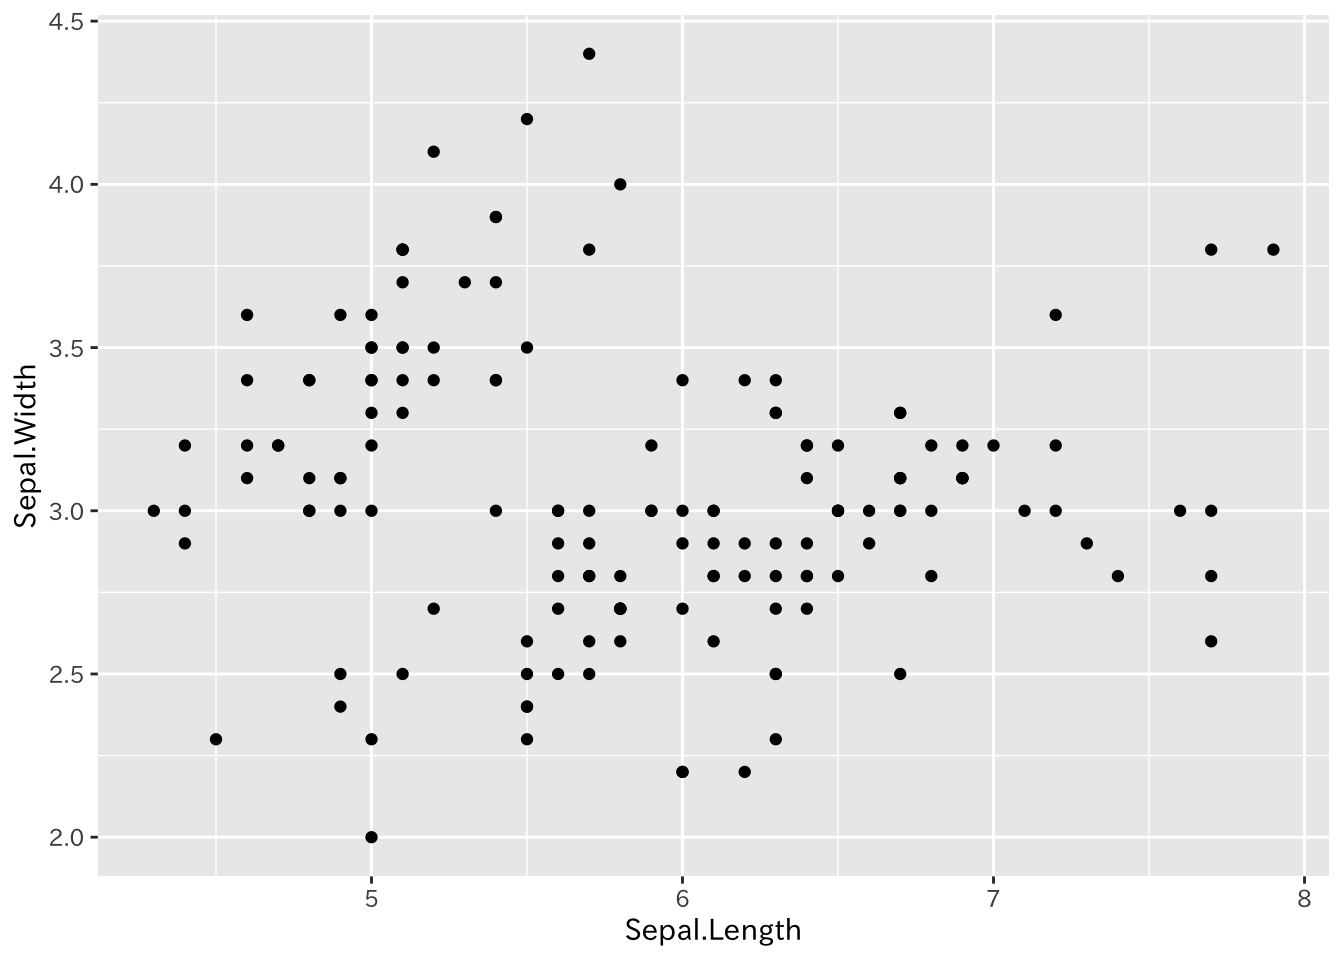
\includegraphics{_main_files/figure-latex/unnamed-chunk-45-1.pdf}
ここでは,あわせてグラフタイトルや軸のラベルも指定した。

ggplotは利用している人が非常に多いので,インターネット上にいくらでも丁寧な解説がある。使い方を覚えるというよりは,グラフを描く必要があるときに,どうすれば目的のグラフを描くことができるかをググりながら使えば良い。

  \bibliography{book.bib,packages.bib}

\end{document}
